%#!platex jou.tex
\chapter{図表の構成}\chaplab{floats}
\begin{abstract}
%%おちゃらけばーじょん
%\yo{渡辺君,先生はもう今年で63になるけど,先生の
%ころは論文なんてみんな手書きだったからね,図も
%自分で雲形定規を使って描いてたよ.それに
%図にはスクリーントーンも工夫して貼ってたよ,懐か
%しいなぁ.君たちの世代はそんなことやったことない
%んだろうねぇ.}\pp{渡辺徹『雲のうえの声』より}
%
%数十年前までは論文作成に必要なものといえば糊とは
%さみとカッターなどのアナログな道具でした.今では
%ほとんどの論文を電子的に提出できるようになりまし
%た.{\LaTeX}ではある程度の手順を踏めば非常に高品
%質に電子的な図表の組版が可能です.
レポート・論文に図や表を取り入れる事は読者の理解を助ける事になります.
この章では文書中にどのように図表を構成すれば良いのかを解説します.
\end{abstract}

\section{一般的な取り決め}

以下は一般的なレポート・論文作成における図表に関する取り決めです.

\begin{description}
\item[図表の位置] 
 一般的に,論文中において図表は\K{ページの上端か下端に出力します}.
 \K{関係文章よりも前出する事がなければ},本文中に配置する事も
 可能です.ただし,図表の前後に文章が1行だけ取り残されるような事は避ける
 ようにします.\K{図表は中央揃えにします}.このとき図表の左右に
 文章を流し込む事もありますが,原則として図表と本文を区別するため
 に,左右に文章は記述してはいけません.

\item[図表と本文の空き] 
 本文領域と区別するために,図表と本文は1行程度は空きを設けて
 出力します.

\item[図表の注釈] 
 図表に注釈を付け加えるとき,\K{注釈のサイズは
 本文よりも少し小さくし},図表の下部に配置します.

\item[図表見出し] 
 \zindind{図}{の中央揃え}\zindind{表}{の中央揃え}\zindind{図表}{見出し}%
 文書中の\K{すべての図表}に必ず見出し(\K{図表見出し})
 を付けます.図には\KY{図見出し}を, 表には\KY{表見出し}を
 付けます.見出しは図表と同じく\K{中央揃え}にしま
 す.場合によっては,図表見出しは本文に対して,書体とサイズを変更
 して出力する必要もあります.表見出しは\K{表の上部},図見出しは
 \K{図の下部}に配置します.

\item[通し番号] 
 \index{一意}%
 図表見出しには配置した順に\K{一意の通し番号}も表記します.
 これは「38番目の図」という方法でも,「5章の6番目の表」などで
 も構いません.通常,論文などの規模では\KY{章立て}する
 必要に迫られますので,図表見出しに付加する番号は`図~5.6'のように,
 \K{章に連動して番号付け}されます.

\item[\Z{表罫線}] 
 \indindz{表組み}{欧文の}%
 \indindz{罫線}{表の}%
 欧文の\Z{表組み}の場合,\K{縦罫線は原則的に使いません}.
 和文の場合でも,表に使用する罫線は最小にとどめる事になります.
\end{description}

これらの取り決めを守る事により図表に関する一貫性がうまれる事となります.
必ず上記のようにしなければならないというルールはありません.学会や
機関によってはこれとは異なる方針を持っている事もあります.いずれに
しても,何かしらの一貫性を持たせるという基本原則は守るように執筆
する事を心がけるようにすると,読者に親切な表記と言えるでしょう.

%\section{図表の基礎}
\section{\LaTeX での扱い}

%図や表を{\LaTeX}では\Z{浮動体}\pp{\tabref{floats}}
%と呼ばれる場所に一度退避させることができます.このように
%すると{\LaTeX}は{\LaTeX}自身が最適だと思われる場所に図表
%を出力しようと努力します.浮動体として退避させた図や表は
%少し制限の多い条件で組版されます.
レポートや論文においては基本的に図表に対して通し番号を振るために,図表は
\Env{table}環境か\Env{figure}環境に入れ子にします.この場合,{\LaTeX}で
は図表を\KY{浮動体} (\Z{float}) と呼ばれる場所に一度退避させ,最適な位置
に図表を配置しようと試みます\pp{\tabref{floats}}.浮動体として退避さ
せた図表は少し制限の多い条件で組版されます.
\begin{wraptable}[6]{r}{20zw}
\caption{浮動体の種類}\tablab{floats}
\begin{tabular}{lcc} 
\TR
           & \Th{表}          & \Th{図}          \\ 
\MR
入れる環境 & \Env{table}環境 & \Env{figure}環境 \\ 
見出しの位置 & 表の上部 & 図の下部 \\
\BR
\end{tabular}
\end{wraptable}
%\indindz{番号}{図表の通し}\indindz{番号}{表の通し}\indindz{番号}{図の通し}%%%
%表は\Env{tabular}環境で作成し,番号付けしたければ\Env{table}環境中に
%入れ子にします.図は\Env{picture}環境や\indindz{ファイル}{画像}画像ファイルを指定し,番号付
%けしたければ\Env{figure}環境中に入れ子にします.このようにするとそれ
%らの図表は浮動体として扱われます.レポートや論文では図表に通し番号
%を付けるのは必須ですから,全ての表は\env{table}環境の中へ,図は
%\env{figure}環境の中に入れるのが良いでしょう.
%
%{\LaTeX}が内部でどのように,これら浮動体を配置しているのかという難し
%い部分を押さえなければ自分の思い通りの位置に図表を配置することができ
%ない場合が多いでしょう.余り図の出力位置などを気にしなければそれで
%良い問題です.
%
%浮動体を挿入するときに指定するのはその配置場所です.基本的に{\LaTeX}は
%図表をページの最上部か最下部に配置しようとして,それでも無理なときは
%別ページへと出力します.ユーザはこれら浮動体の配置場所を指定する
%ことができます.指定できる場所は\tabref{hudoutai}となります.位
%置指定は複数指定することが可能です.

\indindz{番号}{図表の通し}\indindz{番号}{表の通し}\indindz{番号}{図の通し}%
表 (\Z{table}) は\Env{tabular}環境で作成し,番号付けしたければ
\Env{table}環境中に入れ子にします.
%
図 (\Z{figure}) は\Env{picture}環境や\indindz{ファイル}{画像}%
画像ファイルを指定し,番号付
けしたければ\Env{figure}環境中に入れ子にします.このようにするとそれ
らの図表は浮動体として扱われます.レポートや論文では図表に通し番号
を付けるのは必須ですから,全ての表は\env{table}環境の中へ,図は
\env{figure}環境の中に入れるのが良いでしょう.
\indindz{画像}{浮動体としての}%

%{\LaTeX}が内部でどのように,これら浮動体を配置しているのかという難し
%い部分を押さえなければ自分の思い通りの位置に図表を配置することができ
%ない場合が多いでしょう.余り図の出力位置などを気にしなければそれで
%良い問題です.

\zindind{ページ}{の最下部}%
\zindind{ページ}{の最上部}%
図表を挿入するときに指定するのはその配置場所です.基本的に{\LaTeX}は
図表をページの最上部か最下部に配置しようとして,それでも無理なときは
別ページへと出力します.ユーザはこれら図表(浮動体)の配置場所を指定する
事ができます.指定できる場所は\tabref{hudoutai}となります.位
置指定は複数指定する事が可能です.

\begin{table}
\begin{center}
\caption{浮動体の位置指定}\tablab{hudoutai}
\begin{tabular}{cl}
\TR
\Th{記号} & \Th{浮動体の配置する場所} \\
\MR
\str h & まさにその場所に配置しようと試みます\\
\str t & ページ上部に配置しようと試みます\\
\str b & ページ下部に配置しようと試みます\\
\str p & 浮動体を別ページに配置しようと試みます\\
\str ! & 無理やりその場所に配置します\\
\BR
\end{tabular}
\end{center}
\end{table}
これらの位置指定は\env{table}環境や\env{figure}環境の
\K{任意引数として渡します}.\env{figure}環境で例を示すと
次のように使います.

\begin{InTeX}
\begin{figure}[htbp]
ここに図が入ります.
\end{figure}
\end{InTeX}


%\indindz{見出し}{図の}
%\indindz{見出し}{表の}
%一つここで注意しなければならないことは,図表の見出しの位置です.\KY{図見
%出し}は図の下部に,\KY{表見出し}は表の上部に見出しをつけます.これにつ
%いては\KY{図表見出し}を出力する \Cmd{caption}命令の位置を変えるだけです.
%\begin{Syntax}
%\Cmd{caption}\opa{図表目次用の見出し}\pa{図表見出し\Cmd{label}\pa{ラベル}}
%\end{Syntax}
%
%\env{figure}環境中に表を入れたり,\env{table}環境中に
%図を入れたりすることができます.他にも環境中に文字列
%を挿入することも可能です.

%\begin{Exe}
% \cmd{caption}の使い方.
%\end{Exe}

図表用の見出しを出力するには \C{caption}命令を
\E{figure}/\E{table}環境中で使用します.
\begin{Syntax}
\C{caption}\pa{図表見出し}\C{label}\pa{ラベル}
\end{Syntax}
前述のように表見出しは表の上部に出力するために,\C{caption}
命令を先に,図見出しの場合は,図の後に \C{caption}を先に
記述します.

\env{figure}環境中に表を入れたり,\env{table}環境中に
図を入れたりする事ができます.他にも環境中に文字列
を挿入する事も可能です.

一般的なレポート・論文等においては
図表を文章中で参照するときは「上の図は何々」や「前述の図は何々」
と参照してはいけません.必ず\K{付加した通し番号}で「図~3.8は
何々」として \C{ref}命令で参照します.そのためには \C{label}命令で
ラベルを付け加える事になります.間違っても\K{手動で図表の番号を
書かないで下さい}.%番号の参照は \LaTeX の\secref{xr}を参照して,



\section{表}
\LaTeX で表を作るために三つの環境が用意されています.
\begin{description}
 \item[\Env{tabbing}環境] 
   タブを制御する事によって表を作成する.
 \item[\Env{tabular}環境] 
   高度な表も作成する事ができる汎用的な表作成環境.
 \item[\Env{array}環境]
   \env{tabular}環境と機能は類似しているが数式の
   行列などに使われる事が多い.
\end{description}
\env{array}環境は
\secref{math:array}にて紹介しています
のでそちらを参照してください.\env{tabbing}環境
も簡単に表が作成できる環境なのですが,\env{tabular}
のほうが記述が楽だと思いますので,ここでは\env{tabular}
のみを紹介します.\env{tabular}環境は次のように
記述します.
\begin{Syntax}
\verb|\begin{tabular}|\pa{列指定子}\\
$\begin{array}{*6c}
\text{要素}_{11} &\verb+&+ & \dots &\verb+&+ & \text{要素}_{1n}  & \verb+\\+\\
\vdots &\verb+&+ & \ddots&\verb+&+ & \vdots  & \verb+\\+\\
\text{要素}_{m1} &\verb+&+ & \dots &\verb+&+ & \text{要素}_{mn}  & 
\end{array}$\\
\verb|\end{tabular}|
\end{Syntax}
行列とほぼ同じです.違うのは数式環境には入れなくて
も良いという事です.

\indindz{列指定子}{表中の}%
{\KY{列指定子}}とはその\env{tabular}環境における%
\indindz{罫線}{表中の}%
表の列数や縦方向の罫線などを決めるものです.
\env{tablar}環境で使用できる主な列指定子は
\tabref{graphic:tabular}の通りです.
\begin{table}[htbp]
\begin{center}
\caption{\texttt{tabular}環境の主な列指定子}
\tablab{graphic:tabular}
\begin{tabular}{cl}
\TR
 \Th{列指定子} & \Th{意味}\\
\MR
\str l & 行列の縦1列を左揃えにする\\
\str c & 行列の縦1列を中央揃えにする\\
\str r & 行列の縦1列を右揃えにする\\
\str | & 縦の罫線を引く\\
\str {||} & 縦の2重罫線を引く\\
\str @\pa{表現} & \va{表現}を縦1列追加します\\
\str p\pa{長さ} & ある列の幅の\va{長さ}を直接指定します\\
\str *\pa{回数}\pa{列指定子} & 回数分だけ\va{列指定子}を繰り返す.\\
\BR
\end{tabular}
\end{center}
\end{table}
\env{tabular}環境における各要素\pp{成分}は
\Z{アンパサンド}\qu{\texttt{\&}}で区切ります.
\index{"&@\verb+&+!tabular@\texttt{tabular}環境の\zdash}%
\glossary{"&@\verb+&+!tabular@\texttt{tabular}環境の\zdash}%
\qu{\texttt{\bs\bs}}を行の終わりとしますので
例えば1行3列の表は次のようになります.
\begin{InOut}
\begin{tabular}{ccc}
\LaTeX\,2.09 & \LaTeXe & \LaTeX\,3\\
\end{tabular} 
\end{InOut}

横方向に罫線を引くには \C{hline},
要素の中で縦の罫線を引くときには \C{vline}など
を使います\pp{\tabref{tabular:lines}}.
\begin{table}[htbp]
\caption{\texttt{tabular}環境中での罫線の命令}
\tablab{tabular:lines}
\IOmargin\makebox[0pt][l]{
\begin{tabular}{lp{22zw}}
\TR
 \Th{命令} & \Th{意味}\\
\MR
\Cmd{hline}& 
   横に引けるだけの罫線を引きます\\
\cmd{hline}\cmd{hline}&
  引けるだけの2重の\Z{横罫線}を引きます\\
\Cmd{vline}& 
   要素の中で引けるだけの縦罫線を引きます\\
\Cmd{cline}\pa{範囲}& 
   要素の罫線を行の範囲を指定して引きます\\
\Cmd{multicolumn}\pa{数値} & 行をつなげて列指定子通りに要素を出力します\\
\multicolumn{1}{r}{\pa{要素}\pa{列指定子}} & \\
\BR
\end{tabular} \IOlabel}
\end{table}

横方向の罫線を引くには \Cmd{hline}を,
行を連結するには \Cmd{multicolumn}を使います.
\begin{InOut}
\begin{tabular}{|c|c|c|}
\hline\hline
\multicolumn{3}{|c|}{{\LaTeX}}\\
\hline
\LaTeX\,2.09 & \LaTeXe & \LaTeX\,3\\
\cline{2-3}
\end{tabular} 
\end{InOut}

罫線を利用して迷路のようなものも作れます.
\begin{InOut}
\begin{tabular}{|ccc|c|c|}
\hline
& \multicolumn{1}{|c}{ } & & 
      \multicolumn{1}{c}{} &  \\
& \multicolumn{1}{|c|}{} & & & \\
\cline{2-2}
 &  &  &  &   \\\cline{1-2}
& \multicolumn{1}{c|}{} &  & & \\
\cline{2-2}
&  & \multicolumn{1}{c}{} & & 
      \multicolumn{1}{c}{}  \\
\hline
\end{tabular} 
\end{InOut}
%
\index{論文!\zdash における図表}
レポートや論文では表には表見出しを付けて
中央揃えにするのが望ましいと思われますので
以下のようなフォーマットになります.

\begin{InTeX}
\begin{table}[htpb]          
 \begin{center}              
 \caption{表の出力例}\label{tab:tabular:example}  
  \begin{tabular}{llcr}
   \hline
   出力例 & 1 & 2 & 3 \\ \hline
   \LaTeX の遷移& \LaTeX\,2.09  & {\LaTeXe}& \LaTeX\,3 \\\hline
  \end{tabular}              
 \end{center}                
\end{table}                  
\end{InTeX}
上記のソースの出力例が\tabref{nankadame}となります.
\begin{table}[htpb]
 \begin{center}              
 \caption{表の出力例}\tablab{nankadame}  
  \begin{tabular}{llcr}
   \hline
   出力例 & 1 & 2 & 3 \\ \hline
   \LaTeX の遷移& \LaTeX\,2.09  & {\LaTeXe}& \LaTeX\,3 \\\hline
  \end{tabular}
 \end{center}
\end{table}

\begin{Exe}
しかし,さすがに毎回同じような記述をしていたのでは疲れますので,
自前で表用の \env{mytab} 環境を次のように定義します.

\begin{InTeX}
\newenvironment{mytab}[3][htbp]
 {\begin{table}[#1]\begin{center}\caption{#2}\label{#3}}
 {\end{center}\end{table}}
\end{InTeX}

このように定義すれば,次のように簡単に用いる事ができるようになります.
実際に上記の定義を用いてタイプセットし,実行結果を吟味してください.

\begin{InTeX}
\begin{mytab}[htbp]{中央揃えで見出しのある表の環境}{tab:hoge}
\begin{tabular}{lll}
\LaTeX\,2.09 & \LaTeXe & \LaTeX\,3\\
\end{tabular} 
\end{mytab}
\end{InTeX}
\end{Exe}


\begin{Prob}
問題~\ref{prob:maketitle:and} では \C{maketitle} という表題を出力するため
の命令を紹介しました.そこでは \C{and} によって著者を列挙する事ができま
した.それと等価な出力を \Env{tabular} 環境で実装できるかどうか考えて
下さい.
 
おおむね次のような方法でも実装できる事を確認してください.

\begin{InTeX}
\newcommand \AND{\end{tabular}\hspace{1zw}\begin{tabular}[t]{c}}
\newcommand \makeAUTHOR[1]{%
  \begin{center}\begin{tabular}[t]{c}#1\end{tabular}\end{center}}
\makeAUTHOR{夏目漱石 \\  ○○研究所 \\ ○○事業部  \AND
      福澤諭吉 \\  △△株式会社 \\ △△研究所\AND
      芥川龍之介\\ □□大学 □□学部 \\ □□学科}
\end{InTeX}
\end{Prob}


\subsection{表中の脚注}
\indindz{脚注}{表中の}
\env{tabular}環境中での脚注はうまく出力できない
事が多いようです.その場合は \Cmd{footnotemark}
と \Cmd{footnotetext}の二つを使います.
\indindz{番号}{脚注の}%
\begin{Syntax}
\Cmd{footnotemark}\opa{番号}\\
\Cmd{footnotetext}\opa{番号}\pa{注釈内容} 
\end{Syntax}
\cmd{footnotemark}で脚注記号を表示し,
\cmd{footnotetext}に注釈を書きます.
\begin{InOut}
\begin{tabular}{|c|c|c|} \hline 
  一つ目\footnotemark[1] & 
  二つ目\footnotemark[2] & 
  三つ目\footnotemark[3]\\ \hline
\end{tabular} 
\footnotetext[1]{一つ目の脚注です.}
\footnotetext[2]{二つ目の脚注です.}
\footnotetext[3]{三つ目の脚注です.}
\\ちょっと表示が変になっています.
\end{InOut}
上記の方法ではうまくいかない場合は手動で
脚注を付ける事もできます.
\begin{InOut}
\begin{tabular}{|c|c|c|}\hline 
  一つ目${}^{a}$ & 二つ目${}^{b}$ & 
  三つ目${}^{c}$ \\ \hline
\end{tabular} 
{\footnotesize \\ 
$^{a}$表中一つ目の脚注です.\\ 
$^{b}$表中二つ目の脚注です.\\ 
$^{c}$表中三つ目の脚注です.}
\end{InOut}


\subsection{\env{tabular}環境の出力位置}

実は\env{tabular}環境は列指定子の前に任意引数を一つとります.
\begin{Syntax}
\verb|\begin{tabular}|\opa{位置指定子}\pa{列指定子}\\
\va{表を構成するための記述}\\
\verb|\end{tabular}|
\end{Syntax}
これは表の位置と段落の位置を調整するものです.\env{tabular}環境で作成さ
れた表の上部と段落の位置を合わせるときは\qu{\str{t}}を,下部ならば
\qu{\str{b}}を,中央ならば\qu{\str{c}}を選びます.

\begin{InOut}
\newcommand{\testtab}[1][c]{~日本~
\begin{tabular}[#1]{|c|} \hline 
函館\\ 未来\\ \hline\end{tabular}}
\testtab \testtab[t] \testtab[b]
\end{InOut}


\subsection{書籍スタイルの表罫線\zdash\textsf{booktabs}}

日本人のスタイルの慣習として\Z{表組み}で\Z{縦罫線}や\Z{斜線}を使う傾向が
見られるようです.典型的な (\Z{typical}) 日本人が組んだものは下記のよう
になります.
\begin{InOut}
\begin{tabular}{|l||l|l|}
 \hline
 名称   & 型番  & 個数 \\
 \hline\hline
 たわし & TWS01 & 1000 \\ \hline
 石鹸   & SP01  & 5000 \\ \hline
\end{tabular}
\end{InOut}
実際の本作りや欧文での表組みでは上記のような組み方は避けた方が無難です.
\Z{認知心理学}的にもやさしい次のような組み方をお薦めします.
\begin{InOut}
\begin{tabular}{lll}
 \hline
 名称   & 型番  & 個数 \\ \hline
 たわし & TWS01 & 1000 \\
 石鹸   & SP01  & 5000 \\ \hline
\end{tabular}
\end{InOut}
ただ,もう少し本格的にやろうと思えば,\Person{Simon}{Fear}による
\Y{booktabs} パッケージを使うと良いでしょう.こちらの方が書籍に近いスタ
イルとなります.
\begin{Syntax}
\begin{tabular}{*4l}
 \C{toprule}    & \pp{表の最上部に引く} &
 \C{midrule}    & \pp{表の中間に引く} \\
 \C{bottomrule} & \pp{表の最下部に引く} &
 \multicolumn{2}{l}{\C{cmidrule}   \pa{罫線を引く範囲}}
\end{tabular}
\end{Syntax}
\C{toprule} と \C{midrule},そして \C{bottomrule} の三つを
必ず使うようにします.
\begin{InOut}
\usepackage{booktabs}
\begin{tabular}{lll}
 \toprule
 品名 & 番号 & 個数 \\ \midrule
 たわし & 02A & 3 \\
 雑巾   & 55B & 2 \\
 傘     & X2B & 5 \\ \bottomrule
\end{tabular}
\end{InOut}
表の中に半端の罫線を引く場合は \C{cmidrule} 命令を使います.
\C{cmidrule} は \C{multicolumn} などにより列を連結した場合等に
使う事ができると思います.
\begin{InOut}
\usepackage{booktabs}
\begin{tabular}{lll}
 \toprule
 \multicolumn{2}{c}{項目} & \\
 \cmidrule{1-2}
 品名 & 型番 & 個数\\ \midrule
 たわし & 02A & 3 \\
 雑巾   & 55B & 2 \\
 傘     & X2B & 5 \\ \bottomrule
\end{tabular}
\end{InOut}

\subsection{小数点揃え\zdash\textsf{dcolumn}}\seclab{dcolumn}
\E{tabular} 環境などで表を作っていると,\Z{小数点}などで列を\Z{整列}させ
たいときがあります.この場合,手動で次のようにもできます.
\begin{InOut}
 \begin{center}
  \begin{tabular}{|l|r@{.}l|}
   $\sqrt{157}$   & 12 & 53 \\
   $\pi$ & 3 & 141592 \\
  \end{tabular}
 \end{center}
\end{InOut}
しかし,ここは自動的に小数点でそろえて欲しいものです.
小数点などをそろえる一つの方法として \Person{David}{Carlisle} の \Y{dcolumn}
を使う方法があります.
\begin{Syntax}
\str{D}\pa{\TeX での区切り}\pa{DVI での出力形式}\pa{小数部の桁数} \\
\C{newcolumntype}\pa{区切り記号}\pa{入出力に関する設定} 
\end{Syntax}
と定義する事により,小数点 `.' に限らず,なんらかの区切りで
列を整列できます.
\begin{InOut}
 \usepackage{dcolumn}
 \begin{center}
  \newcolumntype{.}{D{.}{.}{6}}
  \begin{tabular}{|l|.|}
   $\sqrt{157}$ & 12.53    \\
   $\pi$        & 3.141592 \\
  \end{tabular}
 \end{center}
\end{InOut}
\indindz{列指定子}{小数点を揃える}%
\E{tabular} 環境などで直接{列指定子} `D' を使う事もできます.
上記の場合はあらかじめ\Z{ピリオド} `.' を列の整列用の指定子として
登録しています.



\subsection{表における行の連結\zdash\textsf{multirow}}

\E{array}/\E{tabular} 環境で表などを作成していると,列の連結を
行なう事がしばしばあります.
\begin{InOut}
\begin{tabular}{lll}
\multicolumn{2}{c}{中央} & 右側\\
 左側 & 中央 & 右側\\
\end{tabular}
\end{InOut}
しかし,行の連結となると結構面倒です.そこで \Person{Jerry}{Jeichter}と
\Person{Piet}{Oostrum}による \Y{multirow} パッケージを使えば良いでしょ
う.
\begin{Syntax}
\C{multirow}\pa{行数}\pa{幅}\pa{要素}\\
\C{multirow}\pa{行数}\string*\pa{要素} 
\end{Syntax}
星を付けた場合は\va{要素}をLRモードで組んだときの幅で表を配置します.
まずは行を連結しない場合です.
\begin{InOut}
\usepackage{multirow}
\begin{tabular}{|l|l|l|}
\hline
\multicolumn{2}{|c|}{新商品} & 
  旧商品\\ \hline
 なべ & やかん & たわし\\ \hline
\end{tabular} 
\end{InOut}
次は行を\va{要素}分の幅で連結した場合です.
\begin{InOut}
\begin{tabular}{|l|l|}
 \hline
 \multirow{2}*{新商品}
   & なべ\\
   & やかん\\ \hline
 旧商品 & たわし\\ \hline
\end{tabular} 
\end{InOut}
最後に全角 1 文字分の幅で行を四つ連結させた例です.ただし,
最後の行が 3 文字分あるため,幅の指定は効力がありません.
\begin{InOut}
\begin{tabular}{|c|l|}
 \hline
 \multirow{4}{1zw}{新商品}
   & なべ \\
   & やかん \\
   & コップ\\
   & 洗剤 \\ \hline
 旧商品  & たわし \\ \hline
\end{tabular}
\end{InOut}

%\begin{comment}

\subsection{ページを跨ぐ表\zdash\Y{longtable}}\seclab{longtable}

要素が非常に多い時は,表がページに収まりきらない場合があります.
このような場合は \Person{David}{Carlisle}の \Y{longtable} パッケージでも使
いましょう. \Y{longtable} パッケージを読み込む事により \E{longtable}
環境が使えるようになります.

ただし, \E{table} 環境中にはいれません.また表の幅をそろえるためには,
\Y{longtable}パッケージの警告が出なくなるまで複数回のタイプセットが必要
になります.

ページが複数ページに跨いでしまったときに,各ページの下部・上部に表示させたい
要素が指定できます.
\begin{Syntax}
\begin{tabular}{ll}
\va{要素} \C{endfirsthead}
 & \pp{表の最初のページの上部にだけ表示する行の要素}\\
\va{要素} \C{endhead}
 & \pp{行がページを跨ぐときページ上部に表示する要素}\\
\va{要素} \C{endfoot}
 & \pp{行がページを跨ぐときページ下部に表示する要素}\\
\va{要素} \C{endlastfoot}
 & \pp{表の最後のページの下部だけに表示する行の要素}
\end{tabular}
\end{Syntax}
具体例を見た方が分かりやすいでしょう.次のような入力があると
すると出力は \figref{longtable} となります.

\begin{InTeX}
\documentclass[a4j,11pt,papersize]{jsarticle}
\usepackage{longtable}
\newcommand\hoge[1][0]{%
  醤油 #1-0 & 32892378923894832894 & 1000 \\
  醤油 #1-1 & 32892378923894832894 & 1000 \\
  醤油 #1-2 & 32892378923894832894 & 1000 \\
  醤油 #1-3 & 32892378923894832894 & 1000 \\
  醤油 #1-4 & 32892378923894832894 & 1000 \\
  醤油 #1-5 & 32892378923894832894 & 1000 \\
  醤油 #1-6 & 32892378923894832894 & 1000 \\
  醤油 #1-7 & 32892378923894832894 & 1000 \\
  醤油 #1-8 & 32892378923894832894 & 1000 \\
  醤油 #1-9 & 32892378923894832894 & 1000 \\
}
\begin{document}
% 表の幅を取得するために \jobname.aux に longtable パッケージは
% 情報を書き出し、2 回目以上のタイプセットで幅をそろえる。
\newcommand\mytablehead{\hline 商品 & 番号 & 個数 \\}
\begin{longtable}{|l|l|l|}
\caption{長いながーい表\tablab{longtable}}
% 表の最初のページの上部にだけ表示する行の要素
\endfirsthead
\hline
\multicolumn{3}{|c|}{前ページの表の続きです。}\\
\mytablehead
\hline
% 行がページを跨ぐとき、各ページの上部に表示する行の要素
\endhead
\hline
\multicolumn{3}{|c|}{この表の続きが次ページにあります。}\\
\hline
% 行がページを跨ぐとき、各ページの下部に表示する行の要素
\endfoot
\multicolumn{3}{|c|}{これでこの表は終わりです。}\\
\hline
% 表の最後のページの下部だけに表示する行の要素
\endlastfoot
% 実際の表の始まり
\mytablehead
\hline
\hoge[1] \hoge[2] \hoge[3] \hoge[4] \hoge[5]
\hoge[6] \hoge[7] \hoge[8] \hoge[9] \hoge[10]
\hoge[11] \hoge[12] \hoge[13]
\hline
\end{longtable}
\end{document}
\end{InTeX}

% not in outer par 
\begin{figure}[htbp]
   \IOmargin
   \makebox[0pt][l]{%
      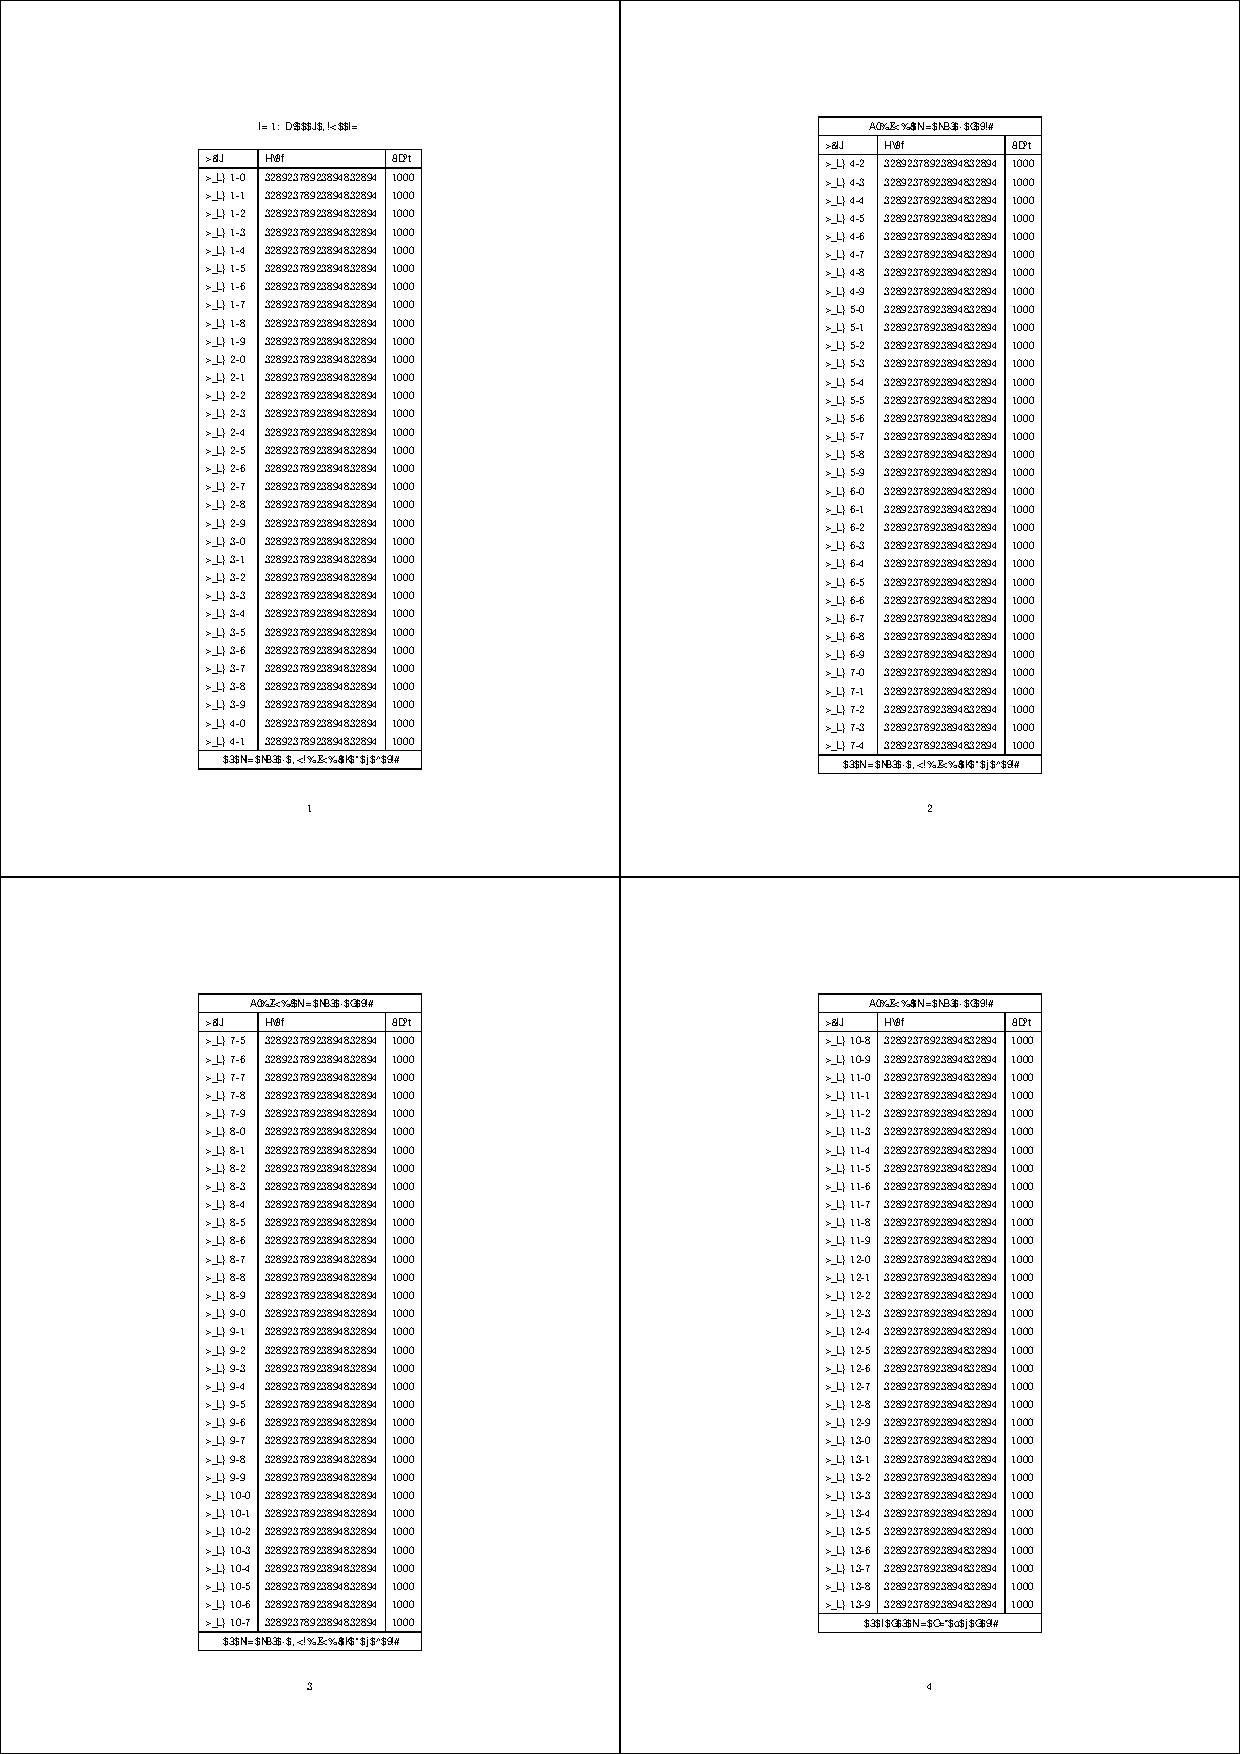
\includegraphics[width=\fullwidth]{images/longtable}%
   \IOlabel
   }%
   \caption{\Y{longtable}の使用例の出力結果}\figlab{longtable}%
\end{figure}

%\end{comment} 

\subsection{表の幅の指定\zdash\Y{tabularx}}\seclab{tabularx}
\LaTeXe の \E{array}/\E{tabular} 環境では列の幅を直接指定できる
列指定子 `\str p\pa{幅}' が用意されていますが,原稿を執筆している段階
ではその幅を決定できない事がしばしばあります.自動的にその幅を求め
てくれるような環境があれば便利です.そこで \Person{David}{Carlisle}の作成
した \Y{tabularx} パッケージを用いる事で \E{tabularx} 環境が使えます.
\begin{Syntax}
\cmd{begin}\verb|{tabularx}|\pa{幅}\pa{列指定子}\\
\va{表を構成する要素}\\
\cmd{end}\verb|{tabularx}| 
\end{Syntax}
具体例を以下に示します.


\begin{InTeX}
\documentclass[a4j,10pt,papersize]{jsarticle}
\usepackage{tabularx}
\makeatletter
\def\hoge{\@tempcnta=\z@ \@whilenum \@tempcnta<10\do{%
   ○○○○\advance\@tempcnta\@ne}。}
\makeatother
\begin{document}
\hoge%
 \begin{center}
  \begin{tabularx}{\linewidth}{|X|X|X|}
   \hline
   \hoge & \hoge & \hoge \\
   \hline
  \end{tabularx}
 \end{center}
\hoge%
\begin{center}
 \begin{tabularx}{\linewidth}{|r|l|X|l|X|}
  \hline
  商品   & 値段 & 説明  & 型番 & 補足事項 \\
  \hline
  鍋     &  500 & \hoge & 59A  & \hoge    \\
  \hline
  やかん &  300 & \hoge & 9JA  & \hoge    \\
  \hline
 \end{tabularx}
\end{center}
\hoge%
\end{document}
\end{InTeX}

上記の入力の出力例は\figref{tabularx}となります.

\begin{figure}[htbp]
 \begin{center}
\makeatletter
\def\hoge{\@tempcnta=\z@ \@whilenum \@tempcnta<10\do{%
   ○○○○\advance\@tempcnta\@ne}。}%
\makeatother
  \begin{tabularx}{\linewidth}{|X|X|X|}
   \hline
   \hoge & \hoge & \hoge \\
   \hline
  \end{tabularx}\par\vskip1em
 \begin{tabularx}{\linewidth}{|r|l|X|l|X|}
  \hline
  商品   & 値段 & 説明  & 型番 & 補足事項 \\
  \hline
  鍋     &  500 & \hoge & 59A  & \hoge    \\
  \hline
  やかん &  300 & \hoge & 9JA  & \hoge    \\
  \hline
 \end{tabularx}
\caption{\Y{tabularx}使用例の出力結果\label{fig:tabularx}}
\end{center}
\end{figure}
%
\E{tabularx} 環境において列指定子 `X' が新たに使えるようになっています.
\E{tabularx} 環境は組むべき表の幅を知る必要があります.`X' が複数の場合は
それぞれの列の幅は均等な長さになります.

\subsection{表作成支援ツール}

{\LaTeX}でゼロから表を組むのは初心者には
辛いかもしれません.GUIベースの
プログラムで表を作成し,それを{\LaTeX}の
\env{tabular}環境の記述に変換するツールを
使うと良いでしょう.Microsoftの\Prog{Excel}
を使っている場合は\Hito{浦壁}{厚郎}の
\Prog{Excel2tabular}\footnote\webEtoT
などがありますので参考にしてください.これらの
プログラムは{Microsoft}の\Prog{Excel}で作成さ
れた表を{\LaTeX}のソースに変換します.

MicrosoftのExcelではなく{OpenOffice.org}の
\Prog{Calc}を使っているならば\Hito{阿部}{昌平}の
\Prog[calc2latex]{Calc2\LaTeX}\footnote \webCtoL
というものもあります.
これを使えばCalcで作成した表を\env{tabular}環境に
変換し,表として{\LaTeX}に貼り付ける事ができます.

最近では直接 \LaTeX から \Prog{Excel} ファイルを読み込める
\Person{Hans-Peter}{Doerr}による \Y{exceltex} パッケージが
あります\footnote{\webExceltex}.
\Prog{Perl}スクリプトを仲介する事で指定したセルやシートを読み込む事がで
きます.

% end of table


\section{図に関する制約と画像の扱い}\label{sec:figure}

図の挿入に関しては大きく分けて2通りの方法があります.一つはペイントソ
フトなどで書いた画像をそのまま取り込む方法, もう一つは{\LaTeX}の
\env{picture}環境で図を直接書く方法です.

\LaTeX には\Env{picture}環境と呼ばれる簡単な\Z{作図}をするための
描画環境が用意されています.この\Env{picture}環境を拡張した
\Y{epic}, \Y{eepic}, \Y{pict2e}などが存在し,ある程度の作図が
できるコマンドが用意されています.\Env{picture}環境とその周辺の詳しい
事は\wasyo{\COMP}\cite{latexcomp}や\wasyo{\GCOMP}\cite{graphicscomp}
を参照してください.

何らかの外部プログラムで作成した BMP, JPEG, PNG, EPS, PDF 等の画像を
\LaTeX に張り込むためには,一般的には\sty{graphicx}パッケージを用います.

\LaTeX 自身では画像ファイルを直接的に扱う仕組みは用意されておらず,
画像ファイルに関する多くの処理をデバイスドライバという外部プログラムに依
存した形を取るため,自分の使おうとしているデバイスドライバがどのような画
像処理に対応しているのかを知ってください.最終的に出力したい文書形式が
PDFならば\prog{\Dvipdfmx},\PS ならば\prog{dvips}を使う事になります.
近年ではDVI 形式から直接 PDF を生成できる\Dvipdfmx を使う事を強く推奨し
ます.\Dvipdfmx を用いる事でBMP, JPEG, PNG, \Z{EPDF}(単一ページのPDF), 
EPS 画像の張り込みが可能となり,さらに DVI ファイルから直接 PDF を生成す
る事ができます.

最近の動向として論文等の提出,印刷には PDF を用いる場合が増えている
ようです.\Dvipdfmx を使えば \LaTeX でそのまま PDF 画像の埋め込み
等もサポートしているため,今後は何かしらの問題がない限り,\Dvipdfmx 
を使うようにすると何かと便利だと思われます.
\zindind{画像}{の張り込み}%

近年まで{\LaTeX}ではEPS以外の画像の張り込みは難しいという都市伝説的な定
説がありましたが,現在は \Dvipdfmx の登場により状況は幾分変化しています
し,これからも変化すると考えられます.



\section{画像ファイルの張り込み}\seclab{gazou}

\LaTeX\ ではビットマップ画像や,曲線の描画などの多くの処理をデバイスドラ
イバと呼ばれる外部のプログラムに依存しています.そのため,\LaTeX\ で画像
ファイルを扱う場合は,まずデバイスドライバを用途別に選択する事になりま
す.


\subsection{デバイスドライバの選択}

各種のデバイスドライバプログラムにおける画像形式に対する対応状況を
\tabref{ddimage}に示します(\genzai での対応状況).
\begin{table}[htbp]
 \begin{center}
  \caption{各種デバイスドライバの画像形式対応状況}\tablab{ddimage}
  \begin{tabular}{ll}
  \TR
  \Th{デバイスドライバ} & \multicolumn{1}{c}{\Th{対応画像形式}}\\
  \MR
  xdvi      & EPS*  \\
  dvips     & EPS   \\
  \Dvipdfmx & EPS*, EPDF, PNG, BMP, JPEG\\
  \Dviout    & EPS*, \Prog{Susie} {plug-in} により他の形式に対応可能\\
  \BR
  \end{tabular}
 \end{center}
\end{table}
星印がついているものは\GS などの外部プログラムを必要とする形式です.

{\LaTeX}で画像を張り込む時,多くの場合は標準的に\sty{graphicx}パッケージを
使う事になります.\Dvipdfmx を使っている場合はパッケージオプション
を\Option{dvipdfmx}とします.

\begin{InText}
\usepackage[dvipdfmx]{graphicx}
\end{InText}

これにより\sty{graphicx}パッケージは\fl{dvipdfmx.def}という設定ファイルを
読み込みます.もしも \Fl{dvipdfmx.def}というファイルが存在しないようであ
れば,以下のURLからファイルを取得し`\str{$texmf/tex/latex/graphics/}'等
のディレクトリにコピーしてください%
\footnote{\url{http://tex.dante.jp/jou1/dvipdfmx.def}}.


古い \TeX/\LaTeX (2006年以前)がインストールされているのであれば,
\option{dvipdfmx}ではなく,\Option{dvipdfm}オプションを指定して,
\Dvipdfmx で PDF をデバイスドライバとします\footnote{何かしらの
理由がない限り \TeX 環境は定期的に更新する事が望ましいです.}.

\begin{InText}
 \usepackage[dvipdfm]{graphicx}
\end{InText}

Unix系OSならば{\PS}のほうが良いでしょうから\Option{dvips}を\sty{graphicx}
パッケージのオプションとします.\prog{dvipsk}であろうが\prog{pdvips}だろ
うが\Option{dvips}オプションを使います.

他には\prog{xdvi}や,Windows であれば \Dviout も指定できます.
Windowsの方で手持ちの画像のほとんどがビットマップで存在するならば\Dviout
をデバイスドライバに選択すれば良いでしょう.\Dviout ではプレビューも印刷も
行えます.
\Dviout の場合は\Dviout がインストールされているフォルダの
\fl{GRAPHIC/LATEX2E/dviout.def}というファイル
を \fl{\$texmf/tex/latex/graphics/} にコピーしてください\footnote{\Dviout の
場合EPS画像を取り込むときは\prog{\GS}にてEPSを\Z{PPM}に変換してから画像
を表示しますから\prog{\Dviout}の\prog{Ghostscript}に関する設定を適切に行っ
てください.}.

EPS画像が多いならばいずれにしても1度EPSからPDFに変換してから
\prog{\Dvipdfmx}を使うのが良いと思われます.%\unixos ならば手持ちの画像を
%EPSに変換して\prog{dvips}を使うことになるでしょう.


\subsection{具体的な手順}

画像ファイルを\LaTeX の文書に張り込むには,一般的に次のような手順を踏む
事になります.

\begin{enumerate}
\zindind{フォント}{のアウトライン化}%
\zindind{PDF}{画像の張り込み}%
\item 外部プログラムでPDFやEPS形式でファイルを保存.保存する時の
      オプションで可能であればフォントはアウトライン化し,カラーに
      依存しないようなファイルとします.
\item 文書のプリアンブルで\sty{graphicx}パッケージを使う事を宣言します.
\item \sty{graphicx}パッケージには\K{デバイスドライバ}を指定します.
      \PS 形式の文書を出力するならば,\Option{dvips}を指定します.PDFを作成し
      たいときは\prog{\Dvipdfmx}を使うために\Option{dvipdfmx}を指定します.
\item EPS以外の画像であれば\LaTeX が解釈できる形で\K{バウンディングボッ
      クス}を指定します.
\item  図を挿入すべき場所に \C{includegraphics}命令を使ってファイル名を
      示します.
\end{enumerate}

デバイスドライバの\Dvipdfmx 等は画像ファイルを扱う事が可能ですが,\LaTeX
は画像ファイルを直接扱う事ができず,画像に関する情報を取得できません.
そのため,\Dvipdfmx において\Z{JPEG},\Z{PNG},\Z{PDF}, \Z{BMP}の画
像ファイルは\KY{バウンディングボックス}という画像の(\Z{原点座標}を含む)
\zindind{画像}{の原点座標}%
サイズ情報を与える事で張り込む事が可能です.一般的には画像の横の長さと縦
の長さのサイズを指定する事となります.バウンディングボックスは
\Va{filename}{img}という画像ファイルがあれば,\Va{filename}{bb}という
ファイルを\sty{graphicx}パッケージが参照するようになっています.

\Dvipdfm に付属する\Prog{ebb}というプログラムで画像のバウンディングボッ
クス情報のファイル \Va{filenam}{bb}を作成できます.対応している画像形式
はJPEG, PNG, PDF です\footnote{ebb以外にも\Prog{identify}コマンドや\Prog{file}コ%
マンドでサイズ情報は知る事ができますし,WindowsやMac~OS~Xであれば%
\Prog{エクスプローラ}や\Prog{ファインダー}にも表示されます.}.

JPEG,PNG,PDF,EPSを直接PDFに張り込めます.具体的な手順として
は,ファイルの存在するディレクトリで
\begin{InTerm}
\type{ebb filename.jpg}
\end{InTerm}
とすれば拡張子が\exten{bb}の\Va{filename}{bb}というファイルが
作成されます.作成された\Va{filename}{bb}を見てみます.

\begin{InText}
%%Title: ./filename.jpg
%%Creator: ebb Version 0.5.2
%%BoundingBox: 0 0 595 842
%%CreationDate: Tue Dec 30 13:04:10 2003
\end{InText}

上記のように\va{ファイル名},\va{作成プログラム}, \va{バウンディングボッ
クス}, \va{作成日時}の情報が出力されます.沢山\Va{filename}{bb}のファイ
ルを保存しておくのが好ましくない場合は,該当する画像ファイルを読み込んで
いる箇所で,次のようにすれば\Va{filename}{bb}がなくても良い事になりま
す.

\begin{InText}
\includegraphics[bb={0 0 595 842}]{filename.jpg}
\end{InText}

使用する画像のファイル名の\Va{ファイル名}{拡張子}は
\qu{\fl{filename.png}}のように\Va{8文字}{3文字}としたほうが互換性の上で安
全です.


\begin{Exe}
仮にファイル名が\fl{image.png}の画像があったとすれば,コンソールから
\type{ebb image.png}として\fl{image.png}用の\fl{image.bb}が作成される事
を確認してください.この\texttt{image.bb}は画像ファイルの縦横を正しく扱
うためのファイルです.\texttt{image.bb} を見れば分かりますが,中身は次
のようなものになっていると思います.

\begin{InText}
%%Title: ./image.png
%%Creator: ebb Version 0.5.2
%%BoundingBox: 0 0 595 841
\end{InText}

\qu{\str{BoundingBox}}とは原点座標と画像の縦横の長さの値です.次にソース
ファイルを以下のようにします.

\begin{InText}
\documentclass[papersize]{jsarticle}
\usepackage[dvipdfmx]{graphicx}
\begin{document}
\centering \includegraphics[width=4cm]{image.png}
\end{document}
\end{InText}

後はいつも通りにタイプセットしてDVIファイルを生成し\prog{\Dvipdfmx}でPDF
を作成します.これにより \fl{image.png}が張り込まれた PDF が生成されるは
ずです.
\end{Exe}

\subsection{張り込みにおけるオプション}

外部プログラムで作成して,すでに存在するような画像は \C{includegraphics}
命令で張り込みます.
\begin{Syntax}
\C{includegraphics}\opa{設定}\pa{ファイル名}
\end{Syntax}

\va{設定}に関しては以下に示すようなオプションが使用できます.

\begin{description}
\zindind{画像}{の高さ}%
 \item[\str{height=}\va{高さ}]
    単位付きで画像の高さを指定します.
 \item[\str{totalheight=}\va{総合的な高さ}]
    単位付きで画像の総合的な高さを指定します.
\zindind{画像}{の幅}%
 \item[\str{width=}\va{幅}]\indindz{幅}{画像の}%
    単位付きで画像の幅を指定します. 
 \item[\str{scale=}\va{数値}]
\zindind{画像}{の拡大}%
    画像の拡大率を指定します. \indindz{拡大}{図の}
 \item[\str{angle=}\va{角度}]
\zindind{画像}{の回転}%
    \K{反時計回りに}画像を回転する角度を指定します. 
 \item[\str{origin=}\va{原点}]
    画像の基準点を決めます. 
 \item[\str{bb=}\va{領域情報}]
    \KY{バウンディングボックス}と呼ばれる画像の大きさと原点座標を指定します.
    画像のどの領域を使うべきかを指定します.\zindind{画像}{のバウンディングボックス}%
    \qu{\str{bb=0 0 640 480}}とすると原点を
    \xy{0}{0}として縦横\qu{$640\times480$}
    の領域を使うようにします.
 \item[\str{viewport=}\va{領域情報}] 
\zindind{画像}{の切り抜き}%
	    画像の利用領域を指定します.切り抜きです.
%	    \str{viewport={30 30 600 40}}
 \item[\str{trim=}\va{領域情報}] 
\zindind{画像}{のトリミング}%
	    画像の端を切り抜きます.
%	    \str{trim={3 3 2 2}}
 \item[\str{noclip}] 
  画像用に使うべき領域を元の画像がはみ出している
  場合に画像を切り抜かないようにします.
 \item[\str{clip}] 
\zindind{画像}{のクリッピング}%
  画像が確保された領域よりも大きい場合は
  切り抜きします.
 \item[\str{draft}] 
 実際に画像を張り込まずに画像が占有す
 るだろう領域が枠による代替表示になり,ファイル名を表示します.
 \item[\str{keepaspectratio}] 
\zindind{画像}{の縦横比}%
 拡大縮小したときに縦横比を保存するようにします.
 \sty{graphicx}パッケージの標準では保存されます.
\end{description}

\begin{Exe}
ご自分の持っている画像\va{ファイル}を\va{デバイス}が
取り込めるのかを試してみください(行頭のパーセントは取り除き,
\fl{images}フォルダに\Fl{gnu-head.pdf}と\fl{gnu-head.bb}があると仮定します).
\begin{InOut}
\usepackage[dvipdfmx]{graphicx}
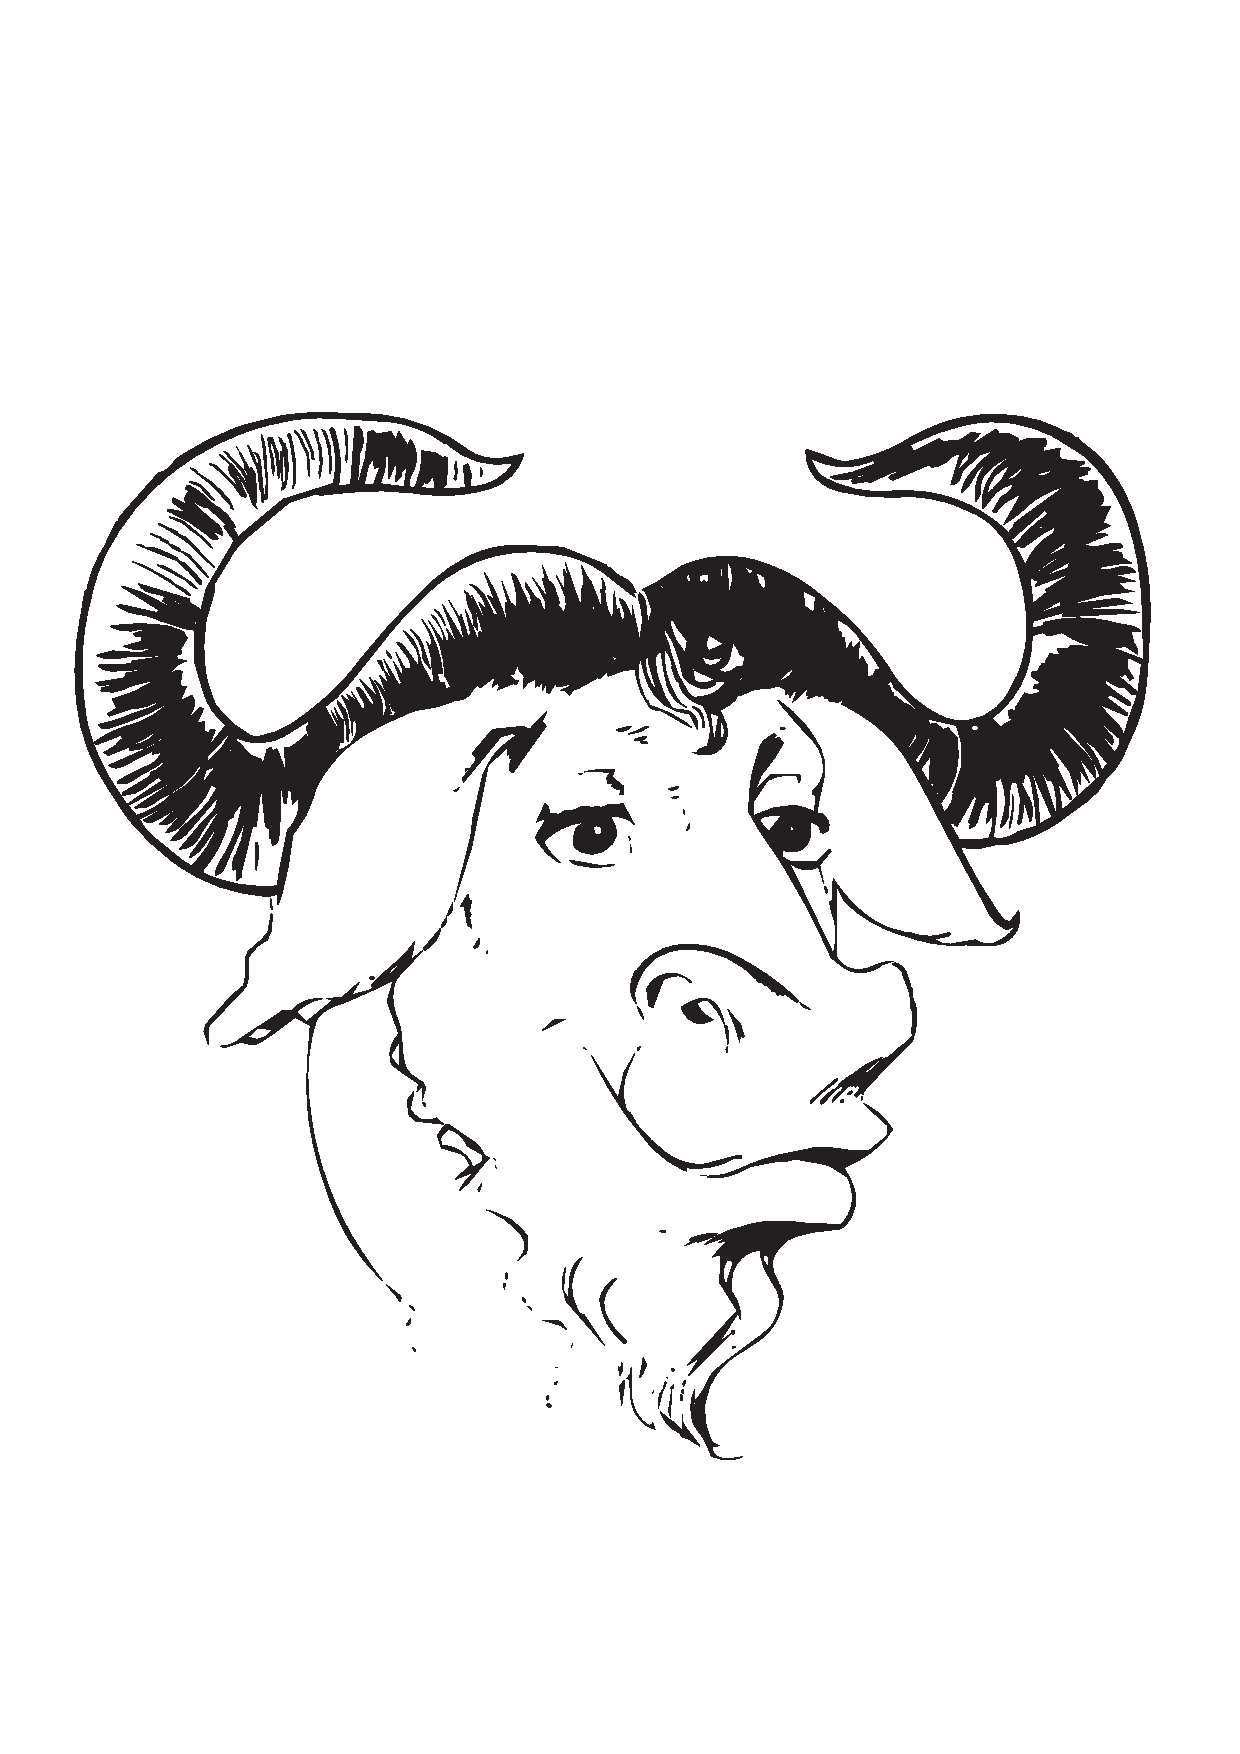
\includegraphics[width=3cm]
  {images/gnu-head}
\end{InOut} 
\end{Exe}

\begin{InOut}
\usepackage[dvipdfmx]{graphicx}
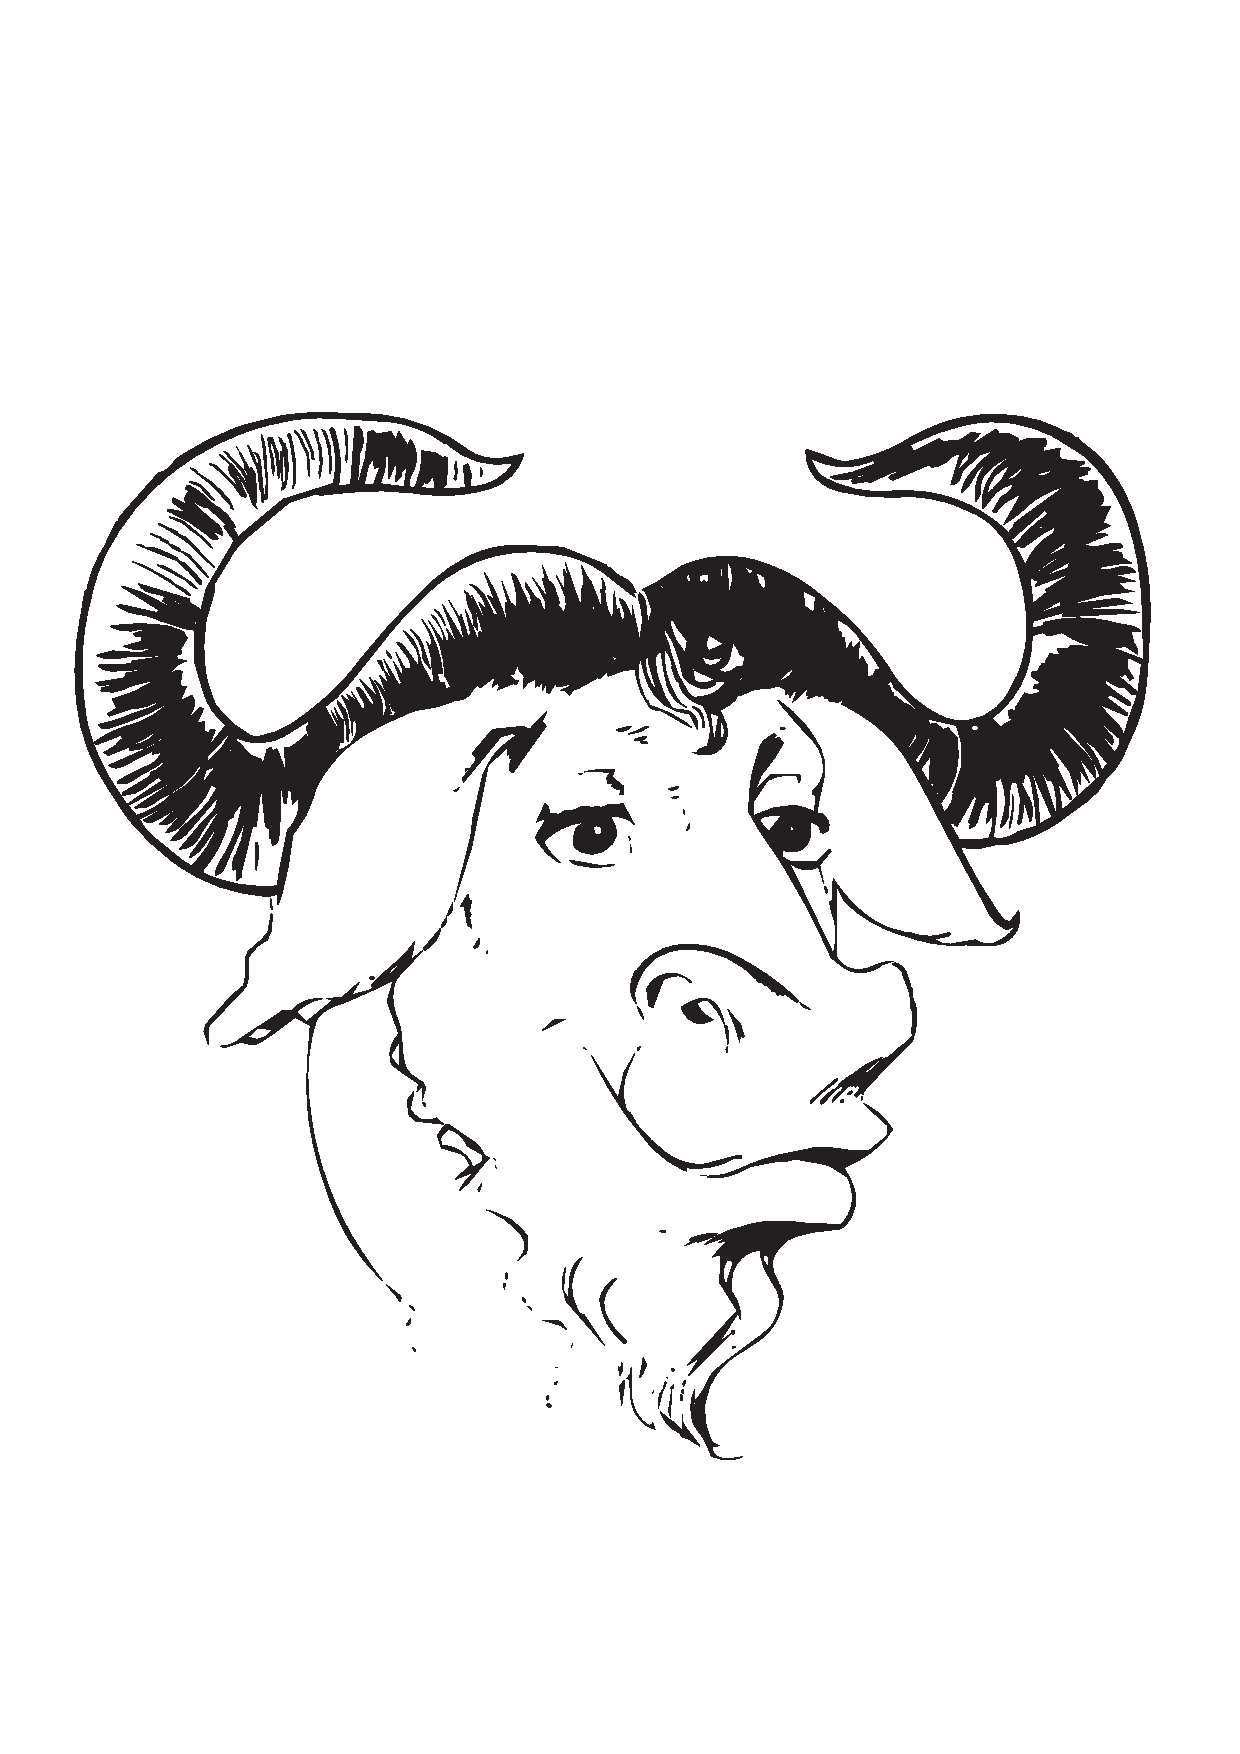
\includegraphics[width=2cm,
  trim=20 20 20 20]
  {images/gnu-head} 
\end{InOut}

\begin{InOut}
\usepackage[dvipdfmx]{graphicx}
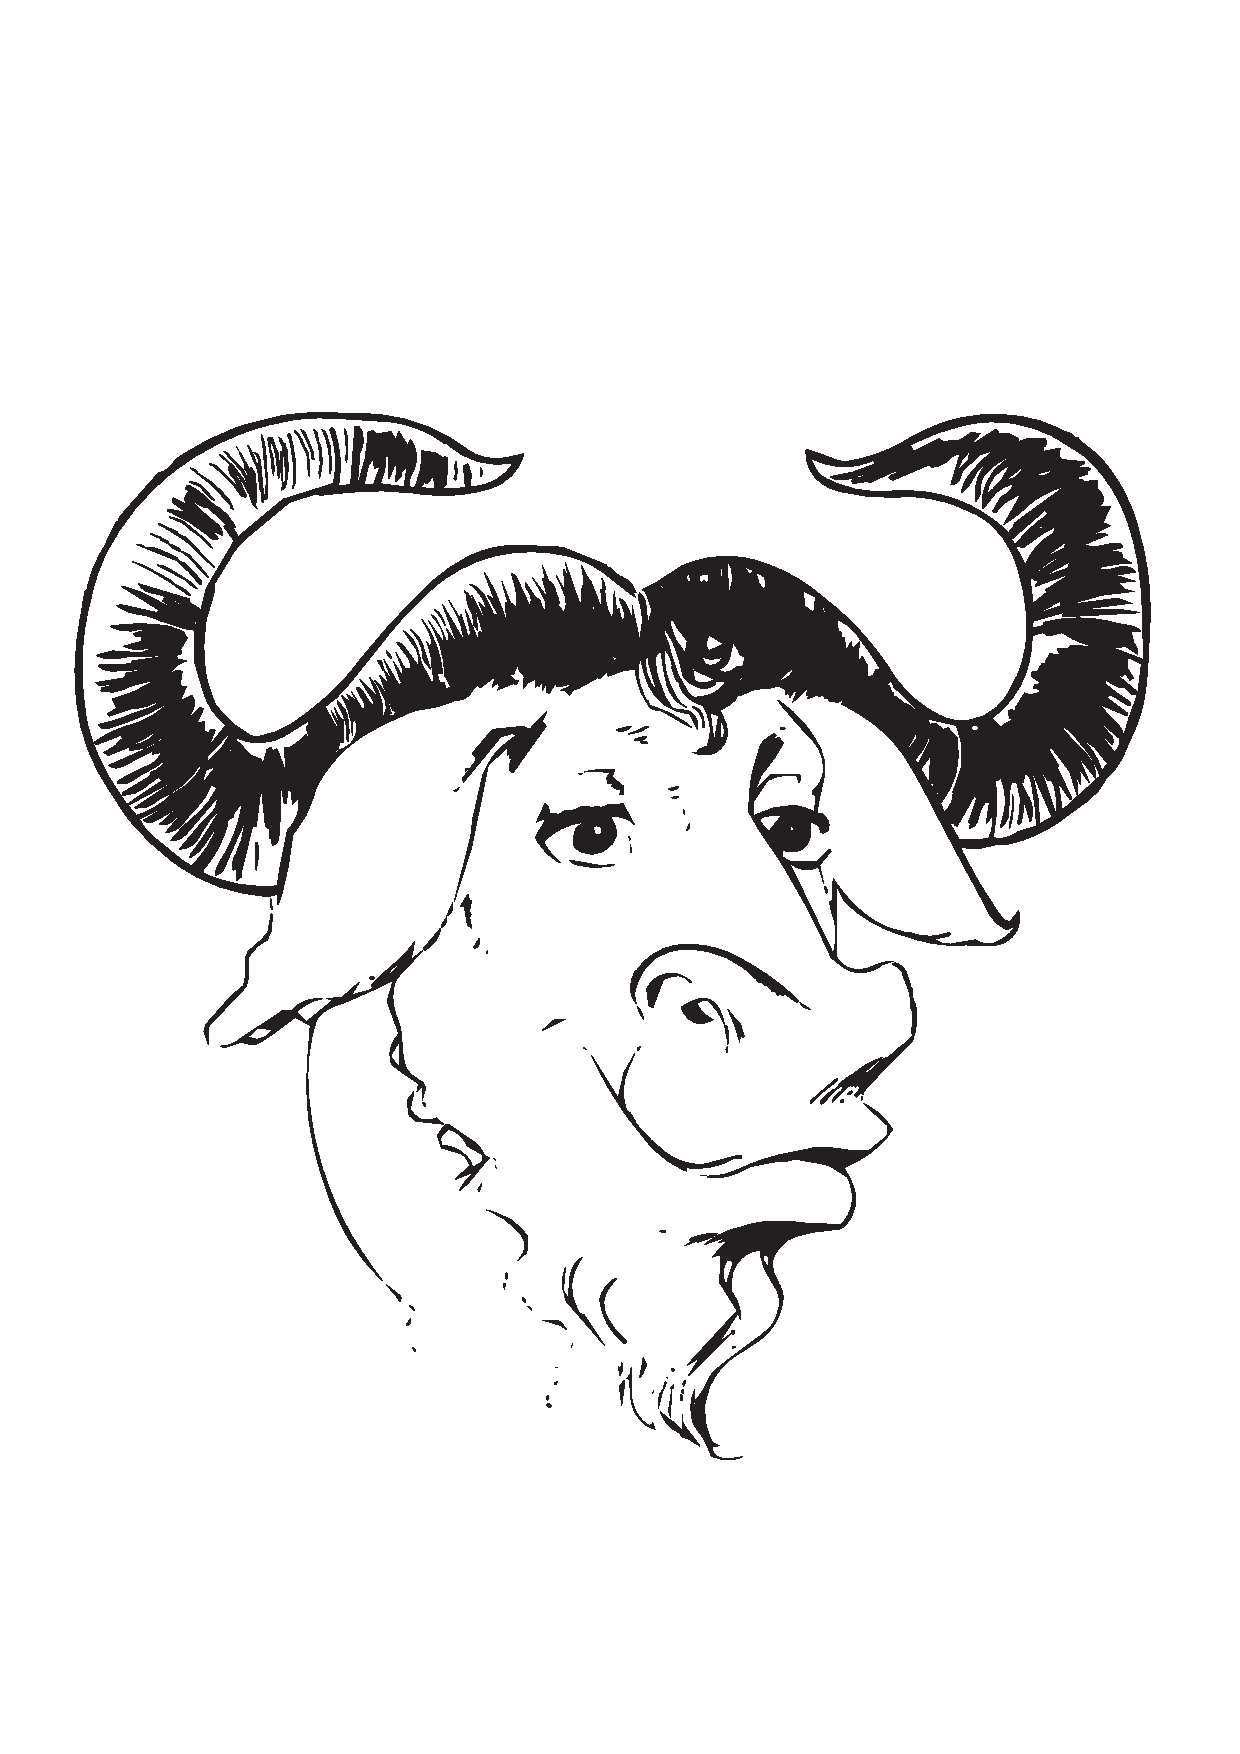
\includegraphics[width=2cm,
  clip,viewport=131 304 459 548]
  {images/gnu-head}  
\end{InOut}

\begin{InOut}
\usepackage[dvipdfmx]{graphicx}
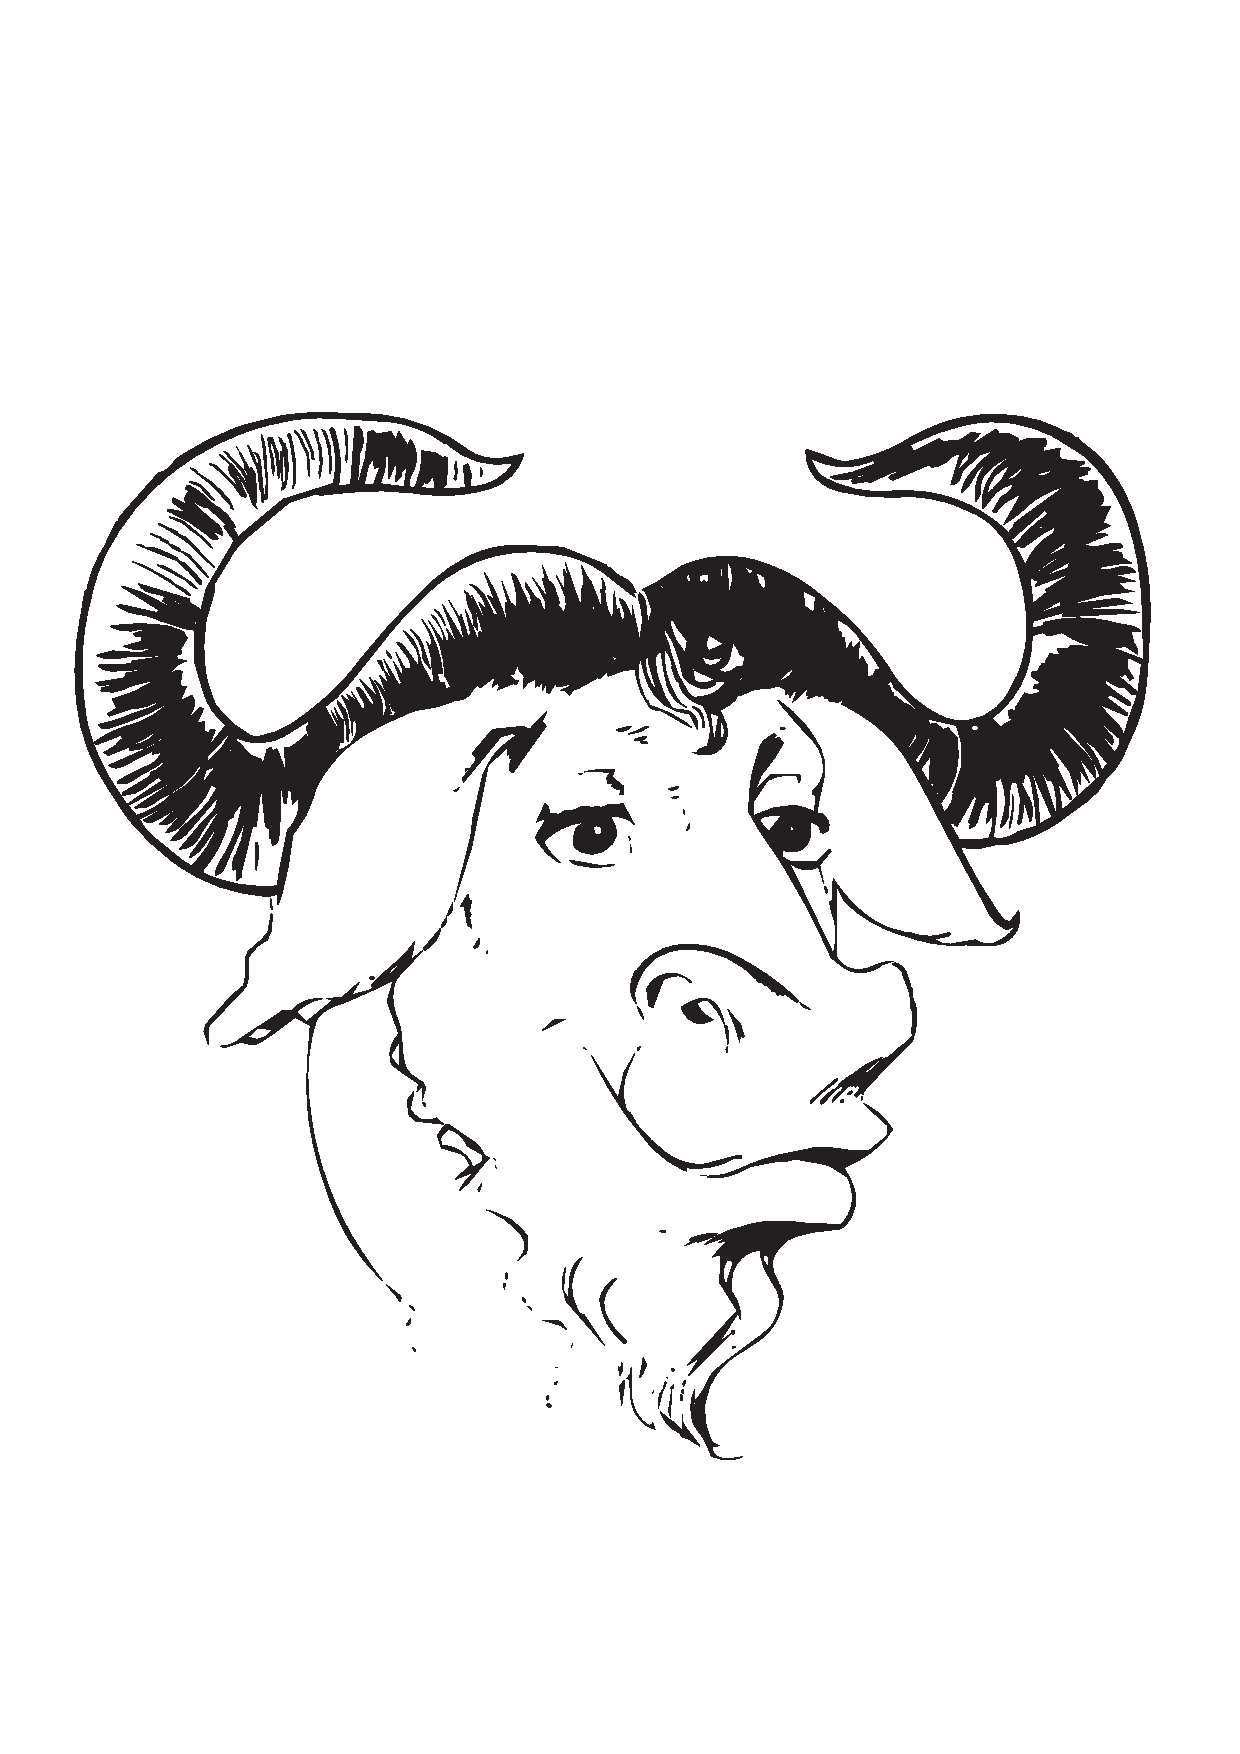
\includegraphics[width=2cm,angle=30,
  clip,viewport=131 304 459 548]
  {images/gnu-head}   
\end{InOut}

\begin{InOut}
\usepackage[dvipdfmx]{graphicx}
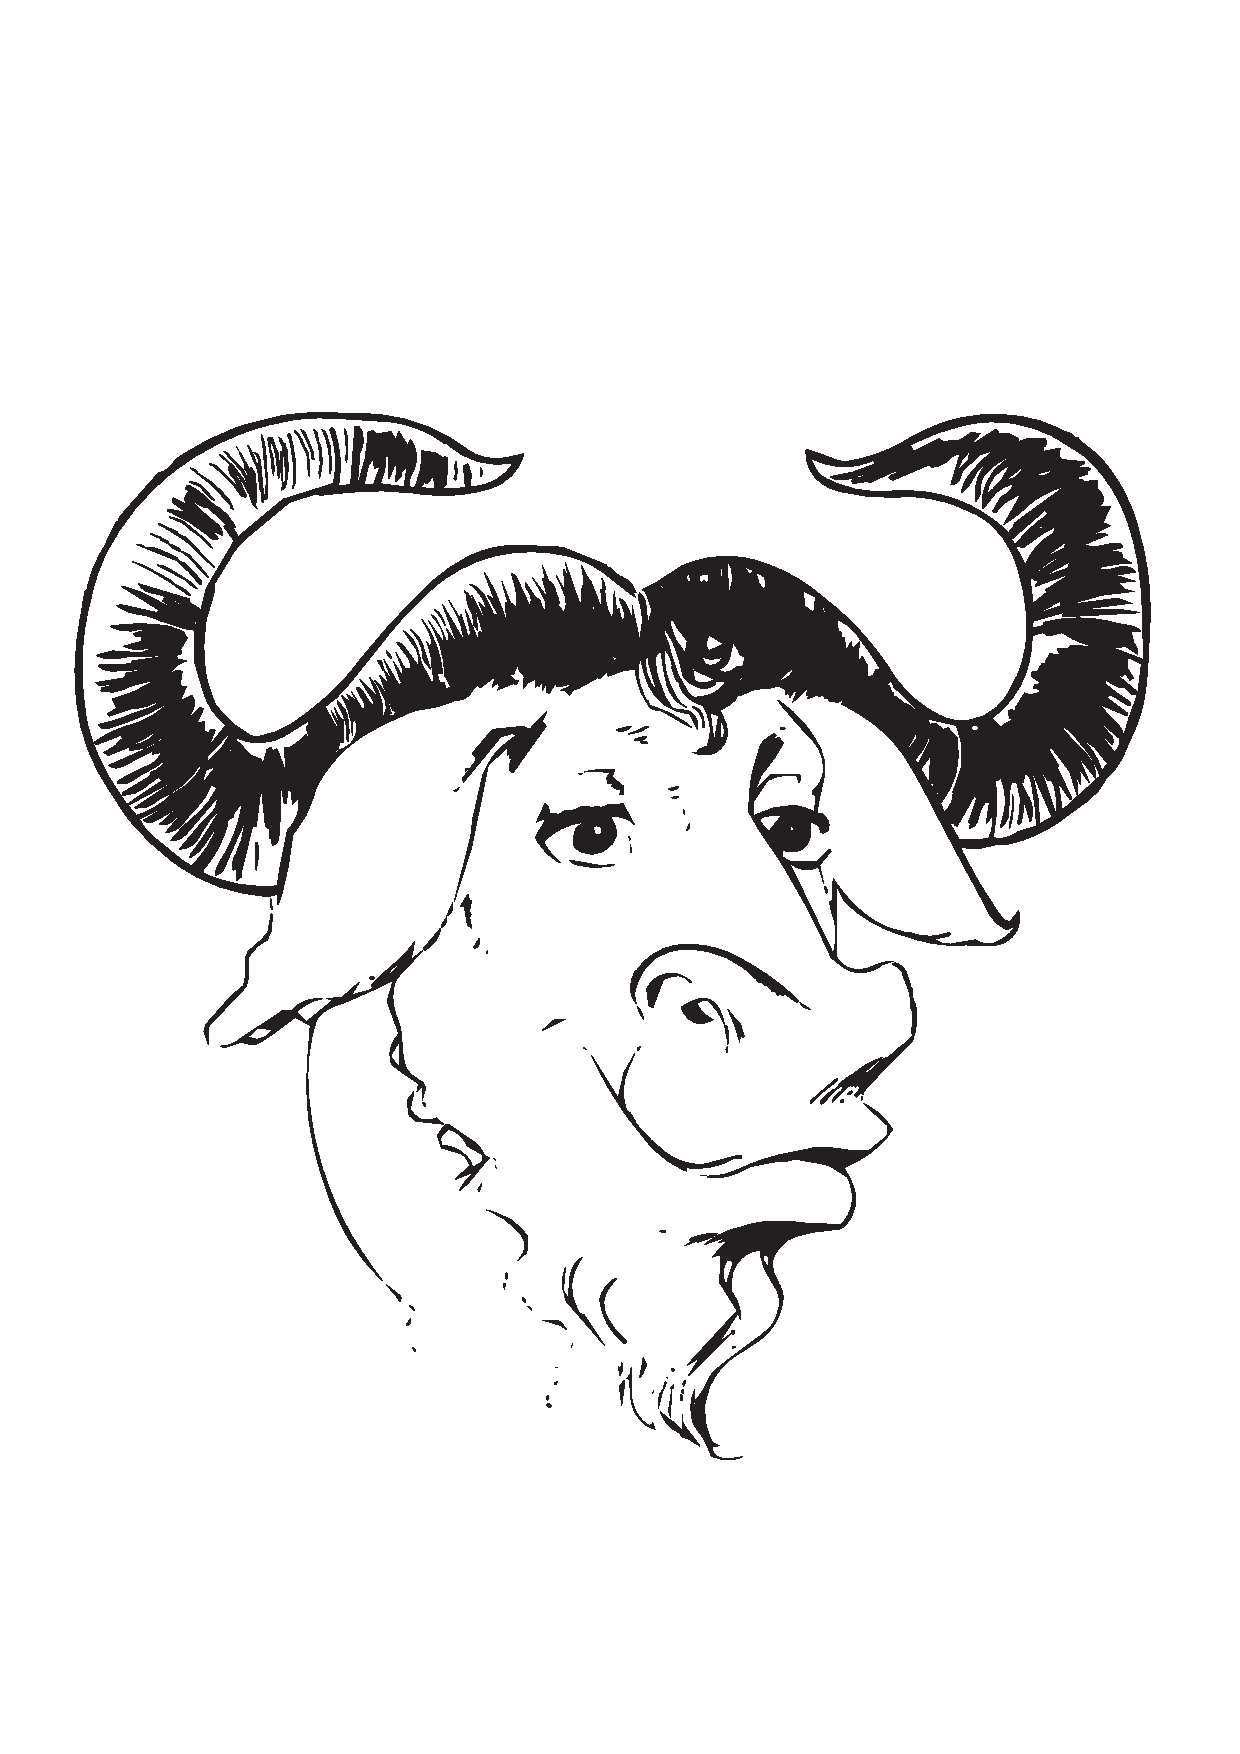
\includegraphics[width=2cm,angle=90,
  clip,viewport=131 304 459 548]
  {images/gnu-head}    
\end{InOut}

\subsection{画像の拡大や回転等の操作}

図などを反時計回りに\kaku{90}回転させる事があるでしょう.
その場合は \Cmd{rotatebox}命令を使います.
\begin{Syntax}
\Cmd{rotatebox}\opa{設定}\pa{角度}\pa{要素}
\end{Syntax}
これは \cmd{includegraphics}の任意引数に
\qu{\str{angle}}を使った事と同じです.
 \cmd{rotatebox}は図に限らずあらゆる要素(表も可能)を
\Z{回転}します.\va{設定}の項目には以下のような
ものがあります.
\begin{description}
\item[\str{origin=}\va{ラベル}] 
 要素を回転するための原点を指定します.%%
 左\qu{\str l},右\qu{\str r},中央\qu{\str c},
 上部\qu{\str t},下部\qu{\str b}が指定できます.
\item[\str{x=}\va{長さ}] 
$x$方向の原点の位置を直接\va{長さ}を指定します.
\item[\str{y=}\va{長さ}]
$y$方向の原点の位置を直接\va{長さ}を指定します.
\end{description}

\indindz{回転}{文字列の}%%%
\begin{InOut}
\rotatebox{70}{文字列など}の
\rotatebox[origin=c]{60}{回転とか}は
\rotatebox[origin=b]{50}{どう}
\rotatebox{30}{ですか?}
\end{InOut}
%
要素を\K{拡大縮小}するには \cmd{scalebox}を
使います.\index{拡大}\index{縮小}\indindz{拡大}{文字列の}
\begin{Syntax}
\Cmd{scalebox}\pa{横の拡大率}\opa{縦の拡大率}\pa{要素}
\end{Syntax}
\va{拡大率}には長さを指定します.\begin{InOut}
\scalebox{2.3}{拡大縮小}\par
\scalebox{3}[1]{拡大縮小}
\end{InOut}

要素の\K{反転}には \cmd{reflectbox}を使います.
\begin{Syntax}
\Cmd{reflectbox}\pa{要素}
\end{Syntax}
\begin{InOut}
\reflectbox{文字列の反転}\par
\reflectbox{山は山}\par
\scalebox{-1}[1]{これも反転}
\end{InOut}

リサイズには \cmd{resizebox}を使います.
\begin{Syntax}
\Cmd{resizebox}\pa{幅}\pa{高さ}\pa{要素}
\end{Syntax}
要素のリサイズ後の幅を\va{幅}に,高さを\va{高さ}にします.
どちらか一方の拡大・縮小率に合わせたいときは\qu{\str!}を
使います.
\begin{InOut}
\resizebox{!}{1cm}{リサイズ}\par
\resizebox{3cm}{!}{リサイズ}
\end{InOut}

以上の \cmd{rotatebox}, \cmd{scalebox}, \cmd{reflectbox},
 \cmd{resizebox}は文字列,表,図,\env{minipage}環境など
の段落などにも使えます.\indindz{回転}{表の}%%
\begin{InOut}
\newcommand{\testtab}{%
\begin{tabular}{|c|}
 \hline \LaTeX\\ \LaTeXe \\ \hline
\end{tabular}}
\rotatebox{80}{\testtab}~
\reflectbox{\testtab}
\end{InOut}

\subsection{\texorpdfstring\Dvipdfmx{Dvipdfmx} におけるEPS画像の扱い}

\Dvipdfmx の場合は基本的にPDF,JPEG,PNG,BMP,MetaPost 形式の
画像しかサポートしておりませんので,EPS形式の画像は何らかの形でPDFに変換
してから取り込む事になります.\LaTeX の原稿中で \C{includegraphics}命
令を用いてEPS画像を張り込んでいる場合は,\Dvipdfmx が DVI から PDF への
変換の段階で \GS プログラムを毎回実行してEPSをEPDFに変換しています.
そのため,\Dvipdfmx をデバイスドライバとして使用しているときには極力
EPSではなく,EPDF画像を張り込むようにします.外部プログラムがPDFでの
保存に対応していないようであれば,あらかじめEPSをEPDFに変換すると
処理速度の向上につながります.

このEPSファイルは\prog{Ghostscript}の\qu{pdfwrite}というデバイスを使って
変換する事がほとんどです.その時に
\Prog{epstopdf}か\Prog{ps2pdf}などを使います\footnote{Vine Linux の場
合は\Prog{ps2jpdf}という日本語フォントを埋め込まない PDF を作成できる
プログラムもあります.\type{apt-get update; apt-get install ps2jpdf}
でインストールできます.}.
\prog{epstopdf}はPDFにEPSの{\BB}を反映してくれます.
\prog{ps2pdf}系を使う場合はPDFに{\BB}がうまく反映されません(\genzai).
以下のようなシェルスクリプト\fl{eps2pdfs}を作成します.

\begin{InText}
#!/bin/bash
EPS=`ls *.eps`;
for fig in $EPS; do
   epstopdf $fig
   $f=`basename $fig .eps`
   grep "^%%BoundingBox:" $fig > $f.bb
done
\end{InText}

\fl{eps2pdfs}を\Z{PATH}の通っている場所(\fl{/usr/local/bin/} など)に複
製したならば
\begin{InTerm}
\type{eps2pdfs}
\end{InTerm}
とすると同ディレクトリのEPSファイルが全てPDFに
変換されます.\Va{file}{eps}があったとすればこれは
\Va{file}{pdf}と\Va{file}{bb}が作成されます.


\subsection{PDF画像の切り抜きと\BB}

%しかし,昨今はEPSではなく,直接PDFしか存在しない場合があり,
%割と \BB を正しく扱えるプログラムというのも少ないようで
%あまり多くはないようだ.%コマンドラインから人が目で見て計測する
何かしらのプログラムで作成したPDFには余計な余白が含まれている
事がしばしばあります.これを自動的に切り抜く方法の一つとして
\Person{Heiko}{Oberdiek}による \Prog{pdfcrop} を使う事により,
PDF画像の余白の切り抜きを行う事ができます(要 \PDFTeX, Perl, \GS).
使い方はコンソールから次のようにするだけです.
\begin{InTerm}
 \type{pdfcrop input.pdf}
\end{InTerm}
これにより \fl{input-crop.pdf}が生成されます.

また,PDFの正確な\BB を取得する一つの方法として
\Prog{pdfinfo} を使う事が考えられます.

\prog{pdfinfo} によって表示される情報は以下のような構成になっています.

\begin{OutTerm}
Creator:        TeX
Producer:       pdfTeX-1.10b
CreationDate:   Sat Apr 15 21:23:00 2006
Tagged:         no
Pages:          1
Encrypted:      no
Page size:      416 x 40 pts
File size:      7995 bytes
Optimized:      no
PDF version:    1.4
\end{OutTerm}

\prog{pdfcrop} によって切り抜きを行った画像であれば,
`\str{Page size: 416 x 40 pts}'を適切に加工すれば\BB と
して使えるようになるでしょう.%`\str{PDF version}'が`1.4'であるため
%\Prog{ebb}では失敗するでしょう.

以下のようなスクリプト \Fl{makebb}を用意します\footnote{\url{http://tex.dante.jp/jou1/makebb}}.

\begin{plainfile}
#!/bin/sh
# 引数として与えられたディレクトリを作業対象とする
cd $1;
# PNG 画像の BoudingBox の生成を ebb により行う
for f in `ls *.png`; do 
   if [ -f `basename $f .png`.bb ] ; then 
      echo "already `basename $f .png`.bb exits."
   else 
      ebb -v $f; 
   fi
done
# JPEG 画像の BoundingBox の生成を ebb により行う
for f in `ls *.jpg`; do 
   if [ -f `basename $f .jpg`.bb ] ; then 
      echo "already `basename $f .jpg`.bb exits."
   else 
      ebb -v $f; 
   fi
done
# PDF 画像の BoundingBox の生成を pdfinfo によって 行う
for f in `ls *.pdf`; do 
   if [ -f `basename $f .pdf`.bb ] ; then 
      echo "already `basename $f .pdf`.bb exits."
   else 
      echo "creating `basename $f.pdf`.bb..."
      pdfinfo $f | grep -e 'Page size:' | \
      sed -e 's/x//; s/Page size:/\%\%BoundingBox: 0 0 /; s/pts//;' \
      > `basename $f .pdf`.bb
   fi
done
\end{plainfile}

これを例えば,適当にアクセス権を与えて \type{makebb img}
とすれば,\fl{img}ディレクトリに存在するPNG, JPEG, PDF画像の
\BB を作成します.

\Z{ストリームエディッタ}の\Prog{sed}がない場合は適当に 
\Prog{Perl}等で実行してください.

%このようにしてEPSからPDFに変換したファイルは
%{\LaTeX}の原稿で次のように取り込むことができます
%(行頭のパーセントは取り除いてください).
%\begin{InOut}
%\usepackage[dvipdfmx]{graphicx}
% \includegraphics[width=3cm]
%    {images/gnu-head}
%\end{InOut}

\subsection{dvipsと\texorpdfstring{\Dvipdfmx}{Dvipdfmx} の併用}

dvipskと\Dvipdfmx の両方を併用している(
\Z{Unix系OS}の方で普段は\PS で印刷していて,
提出用にPDFを作成するなど)場合は\fl{images}ディレクトリ
を作成し,そこに\Va{image}{eps},\Va{image}{pdf},
\Va{images}{bb}の三つのファイルを置きます.次に
原稿中で次のように \C{includegraphics} 命令を使うとき
\K{拡張子を省略します}.

\begin{InText}
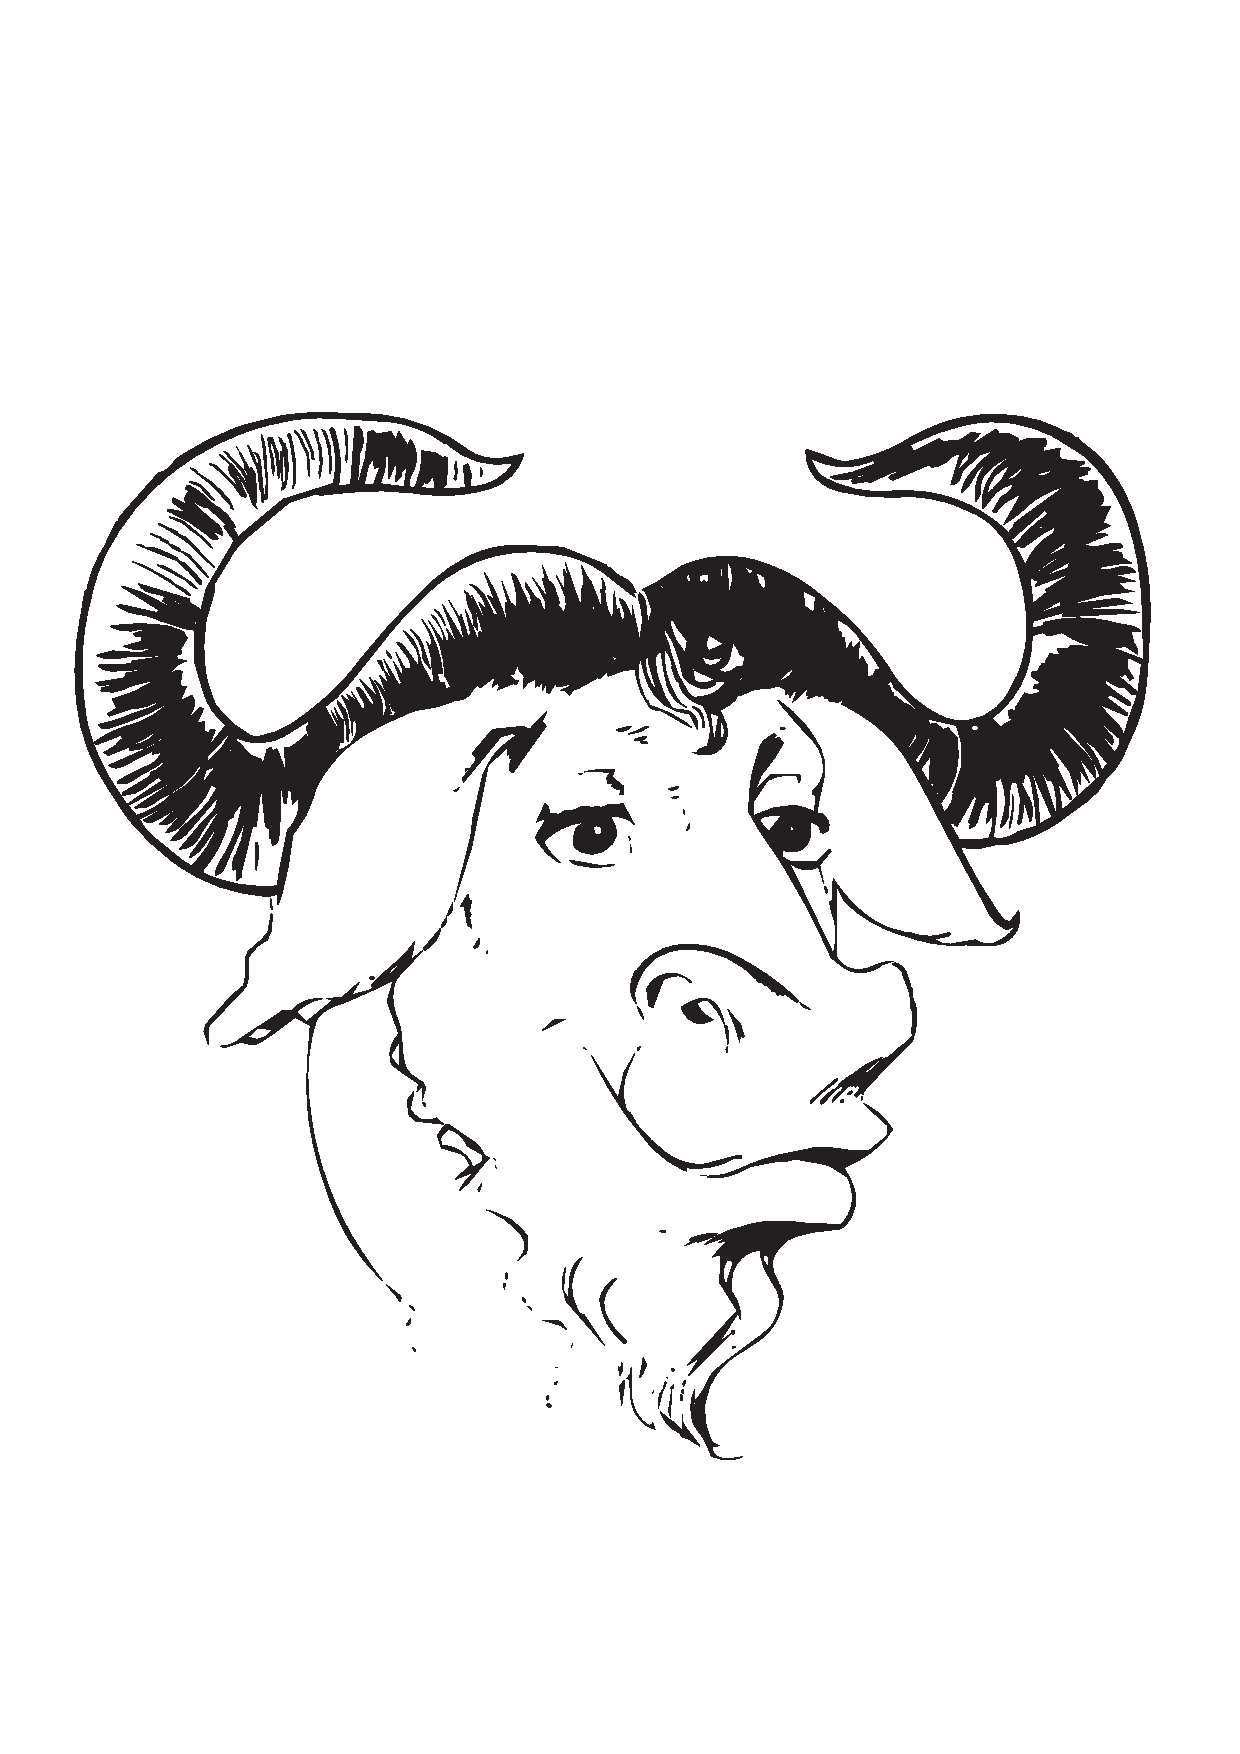
\includegraphics[width=3cm]{images/gnu-head}
\end{InText}

すると\sty{graphicx}パッケージに渡されたパッケージオプションに
従って,張り込まれる画像の優先順位が変わりますので,
\Option{dvips}を指定している場合はEPSが,\Option{dvipdfmx}を
指定している場合はPDFが張り込まれるようになります.
次のように\sty{graphicx}の読み込みの仕方を変更するだけです.

\begin{InText}
%\usepackage[dvips]{graphicx}  % dvipsk   の場合
\usepackage[dvipdfmx]{graphicx} % Dvipdfmx の場合
\end{InText}


\subsection{レポート・論文における図の張り込み}

レポートや論文などで図には\K{図見出し}を付けて\K{中央揃え}に
するのが望ましいと思われますので,次のように使う事になります.

\begin{InText}
\begin{figure}[htbp]
 \begin{center}
   \includegraphics[width=10cm]{images/file.eps}
   \caption{図見出し}\label{fig:samplefig}
 \end{center} 
\end{figure} 
\end{InText}

ただし,これを毎回
書くのは面倒なので次のような図用の\env{myfig}命令を
作成します.

\begin{InText}
\newcommand{myfig}[4][width=.8\linewidth]{%
\begin{figure}[htbp]%
   \centering\includegraphics[#1]{#2}%
   \caption{#3}\label{fig:#4}%
\end{figure}}
\end{InText}

このように定義しておけば次のように簡単に使えます.

\begin{InText}
以上の考察から図~\ref{fig:sample}のような図が得られる.
\myfig[width=100pt,clip]{images/file.eps}{図の張り込みの例}{sample}
\end{InText}

浮動体の図はDVIファイルに出力されるときに思いもよらない場所まで旅をしま
すので,思い通りの場所に図が配置されなくても腹を立てないでください.
そもそも図表に対して\yo{上記の図は何々}とか\yo{下記の図は何々}という表現
は間違いで,全ての図表は\yo{図~3.1は何々}のように番号で参照します.です
から本来は図表がどのような場所に旅立っても困らないはずです.

%HOGE 1037 例題を作成する

\subsection{汎用的な画像の作成と活用}\seclab{excel:kowaza}

\LaTeX と\Dvipdfmx を用いる事で,JPEG, PNG, BMP, EPS, PDF 等の画像を張り
込む事が可能でした.しかし,外部プログラムによってはそれらの形式の画像ファ
イルの\Z{書き出し}(変換)に対応していない場合があります.この場合はある
特定のプログラムから,\Z{仮想プリンタ}に対して画像の内容を送信し,EPSか
PDFで保存するのが手短にできる方法となります.

Windows であれば \Prog{PrimoPDF}等のフリーの変換プログラムがあります.
Mac~OS~XであればOSそのものがPDFでの書き出しに対応しています.%\unixos では

現在お使いの環境に\Prog{Adobe Acrobat}がある場合は,Acrobatを活用し
ていただいて構いません.

\subsection{プログラム特有の処理}\seclab{picture:program}

特定の外部プログラムからグラフや画像を取り込むときには幾つかコツが必
要です.\secref{excel:kowaza}での張り込み方が他のアプリケーション
でも適用できる場合が多いので,上記の方法を試してみてください.

どのプログラムを使用していても最終的に出力したい画像のサイズを元のプログ
ラム側で調節してから{\LaTeX}に張り込むようにすると問題も少ないでしょう.
\sty{graphicx}パッケージの拡大縮小を使うと印刷品質が落ちます.各プロ
グラムにおける設定方法は以下の通りです\footnote{プログラムのバージョンに
よっては幾分操作方法が異なると思います.}.

\begin{description}
\item[\prog{Illustrator}]
  可能であれば文字はアウトライン化します.
  Adobe PDF の互換性では \win{Acrobat 4 (PDF 1.3)}を指定する
  ようにすると,問題が発生しづらいと思われます.
  ツールバーの\win{別名で保存}でファイル形式を\qu{Adobe 
  PDF}として保存します.PDF形式での保存オプションで\yo{サムネー
  ルを埋め込み}の\K{チェックを外して},\yo{圧縮}はしないように
  してください.\Prog{Illustrator}の場合は用紙サイズが切り抜かれ
  ませんので何らかの方法(\Prog{Adobe Acrobat}や \cmd{includegraphics}
  命令の \option{trim} オプション)で切り抜きを行う必要があります.
\item[\Prog{Photoshop}]
  \win{ファイル},\win{複製を保存}を選び\yo{保存形式}
  を\qu{Photoshop PDF}にして保存します.ビットマップ画像は圧縮しないほうが印
  刷品質が良いようです.
\item[Gnuplot] フリーのプロットソフトで \PS, \Y{PSTricks}, \Prog{Tgif},
  \Prog{Illustrator}, \Y{eepic}, \Prog[MetaFont]{\MF},
  \Prog[MetaPost]{\MP}等,多くの形式で画像の書き出しをサポートしています.
  \Prog{Octave}も\Prog{MATLAB}類似でGPLの数値演算ソフトで Gnuplot をもとに
  開発されていますので手順は Gnuplot の場合とほとんど同じです.\Y{eepic}
  パッケージで対処するには,例えば Gnuplot 側で次のようにします.

\begin{InText}
set output 'plotfile1.tex'\\
set term eepic rotated dashed\\
plot x
\end{InText}

すると,カレントディレクトリに\fl{plotfile1.tex}が作成されますから,
\Y{eepic}パッケージ等を用いて,\LaTeX の原稿側で次のように記述します.

\begin{InText}
\documentclass[dvipdfmx]{jsarticle}
\usepackage{graphicx,color,epic,eepic,amssymb}
\begin{document}
\input{plotfile1}
\end{document}
\end{InText}

  この場合は \sty{graphicx}, \Y{epic}, \Y{eepic}, \Y{amssymb}パッケージを
  必要としており,\C{input} 命令でプロットされたグラフ \fl{plotfile1.tex}
  を読み込むようにしてあります.
 \item[R] 
  \index{GNU!\zdash GPL}
  \Z{GPL}の統計解析ソフトで \PS, PDF, \Prog[PicTeX]{Pic\TeX}, \Prog{Xfig}, 
  PNG, JPEG 等の書き出しをサポートしています.

\begin{InText}
pdf()\\
plot(rnorm(10))\\
dev.off()
\end{InText}  

  上記のように\Prog{R}から操作すればカンレントディレクトリにPDF形式の
  グラフ \Fl{Rplots.pdf}が作成されます.
\item[Tgif] \Person{William Chia-Wei}{Cheng}による\Z{QPL}の描画ソフト.EPS
  や PDF 形式に対応しています.PDFに関しては\GS 等の外部プログラムを必要
  とします.
 \item[Mac OS X] Mac OS X の場合は環境自体が PDF に関連した機能を持って
 いるため,PDF 形式で書き出す事により \LaTeX に画像を
 取り込む事ができます.\Prog{Keynotes}, \Prog{Pages}, \Prog{Grapher},
 \Prog{OmniGraffle}等,いずれの場合もメニューバーの \win{ファイル} の
 \win{書き出し} で \win{PDF} を選択する事で PDF として保存できま
 す.\Prog{プレビュー}で \win{選択ツール} によって切り抜きたい領域を
 選択し,それを \win{コピー} した後 \win{クリップボードから新規作
 成} とすればPDF画像の切り抜きもできます.

\zindind{PDF}{とMac OS X}%
\item[\Prog{Mathematica}]
  ツールバーから\win{ファイル}の\win{特殊な形式で保存}を選び
  \win{TeX(X)}を選びます. そうすると数式やグラフなどが自動的に
  {\LaTeXe}形式に保存されます.またグラフはEPS形式で{\fl{
  filename.eps}}という名前で保存されます.{Mathematica}の場合
  出力されるEPS画像の\Z{バウンディングボックス}が正常に
  出力されない事があるので{\LaTeX}で正しく処理できない場合
  があります.出力された\fl{filename.eps}というファイルを
  テキストエディタで開けば次のような記述があります.

\begin{InText}
%%BoundingBox: 91.5625 3.1875 321.938 190
\end{InText}

  これは画像を平面上
  のどこに配置するかを指定するもので,左から
  2次元平面上の始点の$x_0$と$y_0$,終点の$x$と
  $y$に対応します.また,通常はこの値は整数値が
  推奨されます.上記の数値を四捨五入して整数に
  直して取り込んでください.
\item[\Prog{MATLAB}]
  グラフを表示しているMATLABプログラムのウィンドウの
  ツールバーにある \win{ファイル} から \win{エクスポート} を
  選び,ファイルの種類を\qu{EPS Level 2}にし,任意の名前
  をつけて保存します.{Illustrator}形式での出力もサポート
  されていますので,お持ちの場合はグラフを編集できます.
\end{description}

全般的には PDF にさえ変換していれば \Prog{Adobe Acrobat} による編集が
可能となり,さらに \Dvipdfmx を用いれば簡単に画像を張り込む事ができます.
一度PDFに画像を変換すると,そのPDFファイルの編集は\prog{Adobe Acrobat}の
ようなPDF編集プログラムが必要となります.そのため,画像の調整に関しては
元の外部プログラム側で行うようにしてみてください.
\zindind{PDF}{の編集}%

\section{図の張り込みの際の工夫}


\subsection{図を二つ横に並べる}
2段組の場合はそのような事はありませんが,1段組の場合は一つの図だけでは
両脇が開いてしまうのでそこに二つの図を\qu{(a)}と\qu{(b)}として挿入したい
ときがあります.このようなときは\Env{minipage}環境を使います.以下のよう
に入力する例もあります.

\C*{hfill}%
\begin{InText}
\begin{figure}[htbp]
  \begin{minipage}{.47\textwidth}
      \centering%ここに図(a)を入れる
      {\small (a) 初期値$c=0.6$}
  \end{minipage} \hfill
  \begin{minipage}{.47\textwidth}
      \centering%ここに図(b)を入れる
      {\small (b) 初期値$c=1.0$}
  \end{minipage}
  \caption{1段組で横に図を二つ並べる}
\end{figure}
\end{InText}

両方の図の番号を別にしたいときも同様に記述します.
二つ以上横に並べるとき等には\Person{Steven Douglas}{Cochran}による
\Y{subfigure}パッケージを使うとより簡単に記述できる事になります.

\begin{figure}[htbp]
  \begin{minipage}{.47\textwidth}
      \centering
      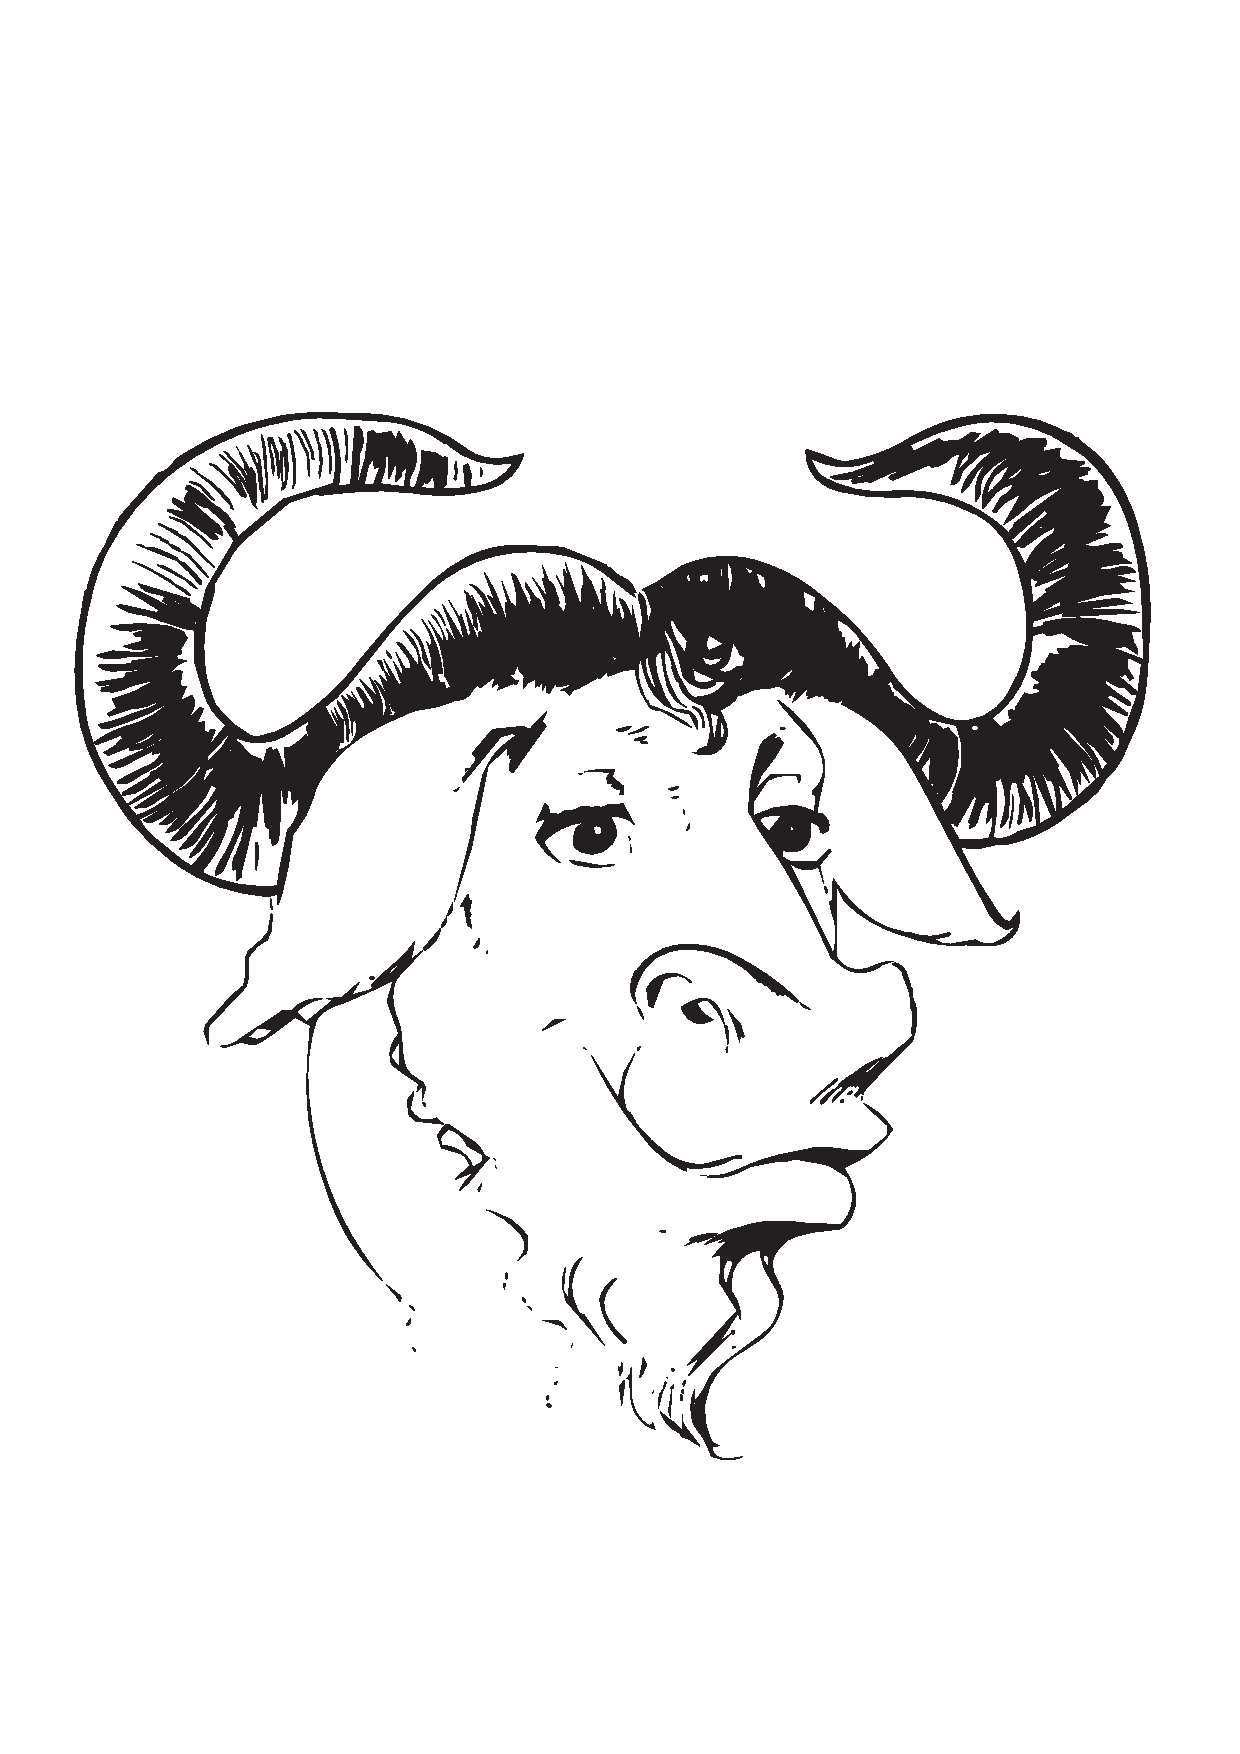
\includegraphics[width=2cm]{images/gnu-head}\\
      {\small(a) 初期値 $c=0.6$}
  \end{minipage}
\hfill
  \begin{minipage}{.47\textwidth}
      \centering
      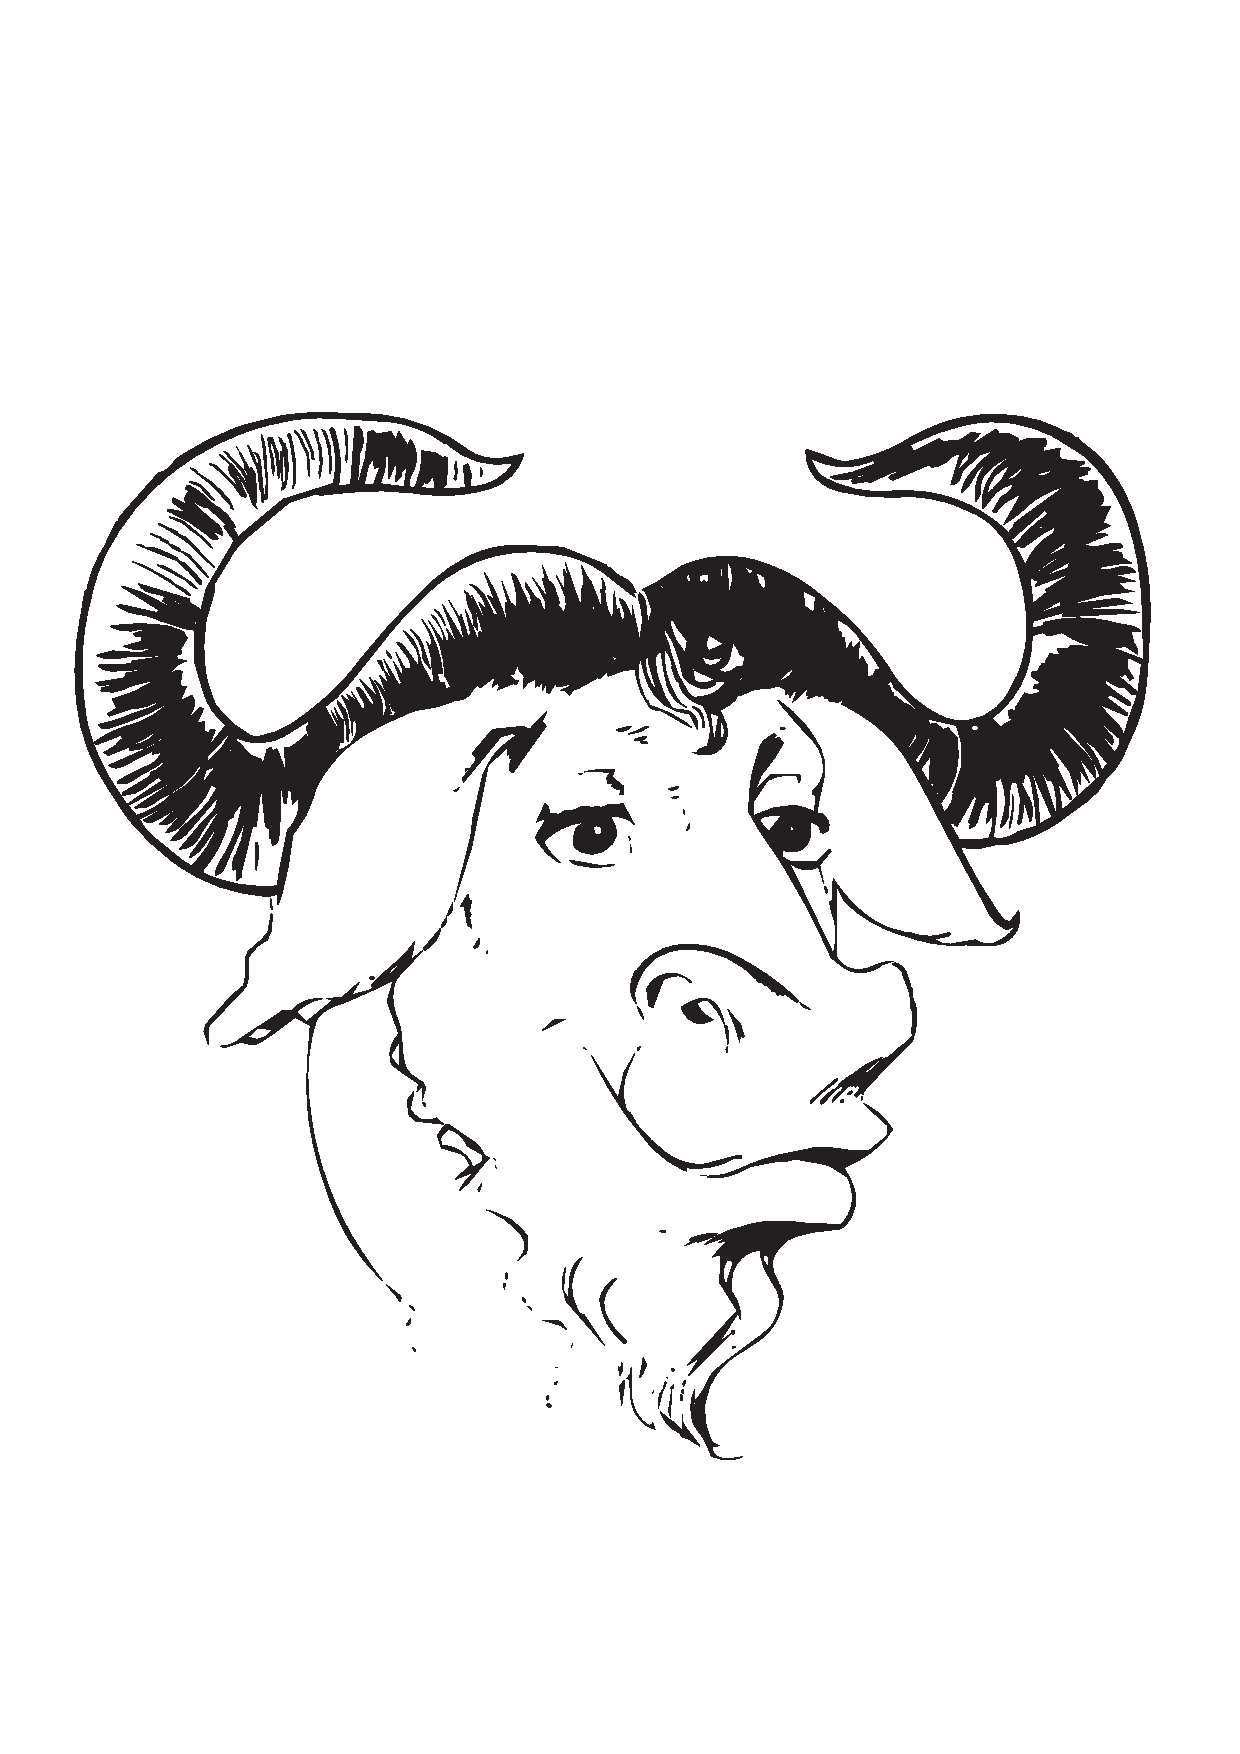
\includegraphics[width=2cm]{images/gnu-head}\\
      {\small(b) 初期値 $c=1.0$}
  \end{minipage}
  \caption{1段組で横に図を二つ並べる}
\end{figure}


\begin{Prob}
ある環境などにおけるその時々の文章幅を保持している \Cmd{linewidth}
という長さがあります.この長さを使うと
その環境において文章幅いっぱいの図を張り込むという事
もできるようになります.

 次の入力を実際に自分でタイプセットし,その結果を吟味してください.
\begin{InOut}
\begin{quote}
  linewidth $=$ \the\linewidth\par
  \begin{quote}
    linewidth $=$ \the\linewidth
  \end{quote}
\end{quote}
\end{InOut}

これにより行の半分程度の長さで図を張り込むならば,次のように
設定できると考えられるでしょう.

\begin{InTeX}
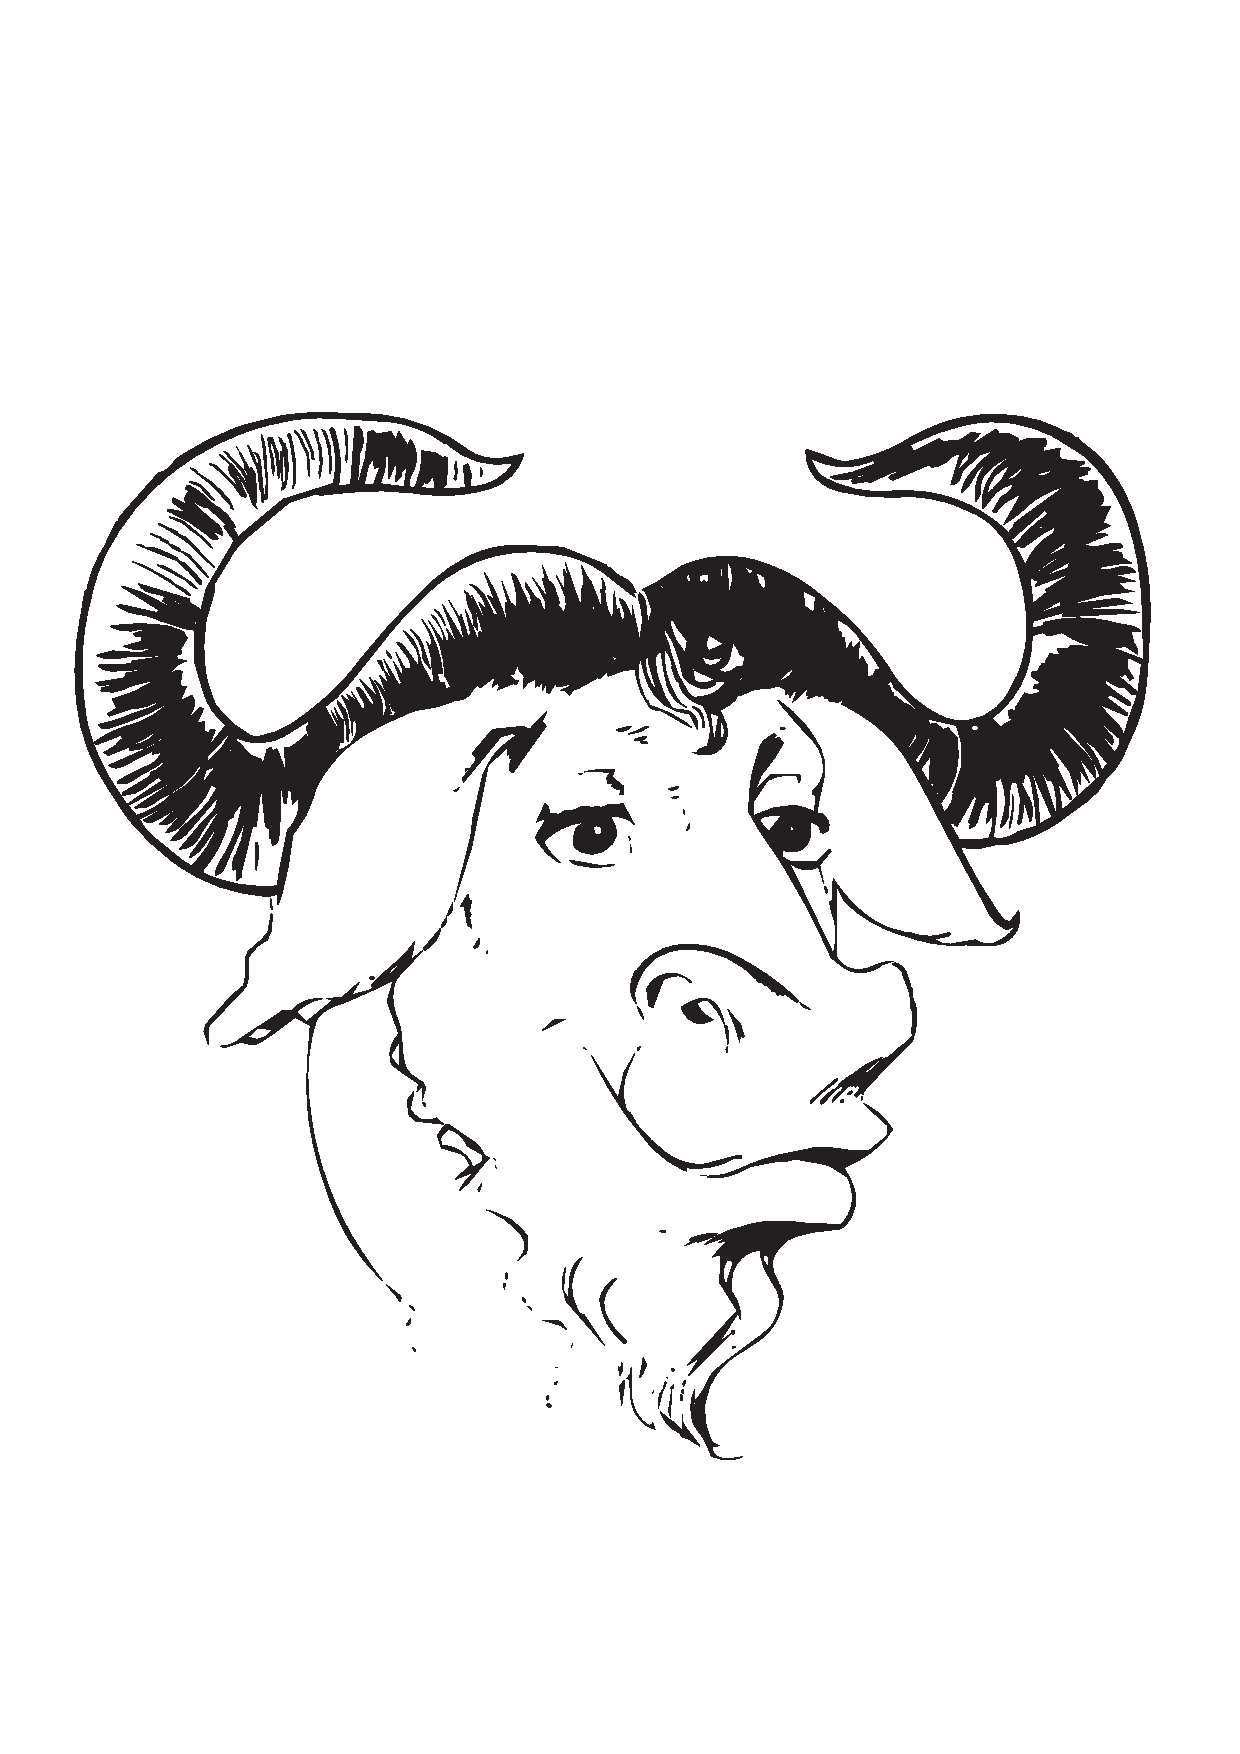
\includegraphics[width=.47\linewidth]{images/gnu-head}\\ 
\end{InTeX}
\end{Prob}

\begin{Prob}
図表を張り込む時に \C{includegraphics}命令に毎回
ディレクトリ名を記述するのが面倒な場合は \C{graphicspath}
命令が使えます.

\begin{Syntax}
 \C{graphicspath}\pa{ディレクトリのリスト}
\end{Syntax}

仮に \fl{images} と \fl{pictures} ディレクトリに画像が
保存されているとすれば,\cmd{graphicspath}は次のように
できるか,実際にタイプセットし,その結果を吟味してください.

\begin{InTeX}
\graphicspath{{images/}{geolay/}}
\end{InTeX}
\end{Prob} 

\subsection{画像に文字を追加する\zdash\textsf{labelfig}}

\zindind{画像}{への文字の追加}%
再編集が難しい画像ファイル,例えば EPS ファイルの上に文字などのラベルを
追加したい場合があります.これには \Person{Raymond}{S\'eroul} と
\Person{Laurent}{Siebenmann} による \Y{labelfig} パッケージが使える
でしょう.
\begin{Syntax}
\C{SetLabels} \\
\va{画像の上に表示したいラベル}\\
\C{endSetLabels}\\
\C{ShowGrid} \pp{必要に応じて}\\
\C{strut}\C{AffixLabels}\va{配置する画像}
\end{Syntax}
\C{SetLabels} から \C{endSetLabels} の中で画像の上に表示したいラベルを
設定します.ラベルを追加するときに必要に応じて \C{ShowGrid} コマンドで
座標を表示します.\C{AffixLabels} の引数に配置すべき画像を指定します.
ラベルは次の書式に従って追加します.
\begin{Syntax}
\va{位置指定}\string(\va{0--1}\string*\va{0--1}\string) \va{ラベル} \verb|\\|
\end{Syntax}
座標指定は \verb|(0.5*0.3)| のように 0 から 1 の範囲で指定します.
\va{位置指定}には 垂直方向の揃えでは \C{T},\C{E},\C{B},
水平方向では \C{L}, \C{R} と無指定\pp{無指定で中央になる}の両方を
組み合わせて使う事ができます.

\C{ShowGrid} によってグリッドを表示するのは原稿執筆段階だけで,
印刷時には表示しないとなれば \Option{draft} オプションを活用します.
ただし,\sty{graphicx} パッケージによって読み込んでいる画像に関しては
\Option{draft} オプションが有効になっているときでも \Option{final} 
オプションを付けたときのように配置してもらいたいので,例えば
次のようにします.

\begin{InText}
% グリッドを表示させるのは draft の時だけにすれば良いことになる
%\documentclass[draft,a4j,11pt,papersize]{jsarticle}
% 印刷時には draft オプションを除けば良いことになる.
\documentclass[a4j,11pt,papersize]{jsarticle}
% graphicx パッケージには final を渡して,いつでも図が表示される
% ようにすると,labelfig の調整が容易になる.
\usepackage[final]{graphicx}
\usepackage{labelfig} 
\end{InText}

例えば次のような入力があれば \figref{labelfig} のような出力に
なります.\C{GridLineWidth}コマンドで罫線の太さを指定できます.

\begin{InText}
\begin{figure}[htbp]
\begin{center}
 \GridLineWidth{.2pt}
 \SetLabels 
  \T\L(.8*.45) 鼻\\
  \T\L(.2*.9) 左の角\\
  \T\L(.7*.9) 右の角\\ 
  \T\L(.75*.3)  口\\ 
  \T\L(.65*.1) 髭\\ 
  \T\L(.3*.6) 左目\\ 
  \T\L(.7*.6)  右目\\ 
 \endSetLabels
 \ifdraft
   \ShowGrid
 \fi
 \strut\AffixLabels{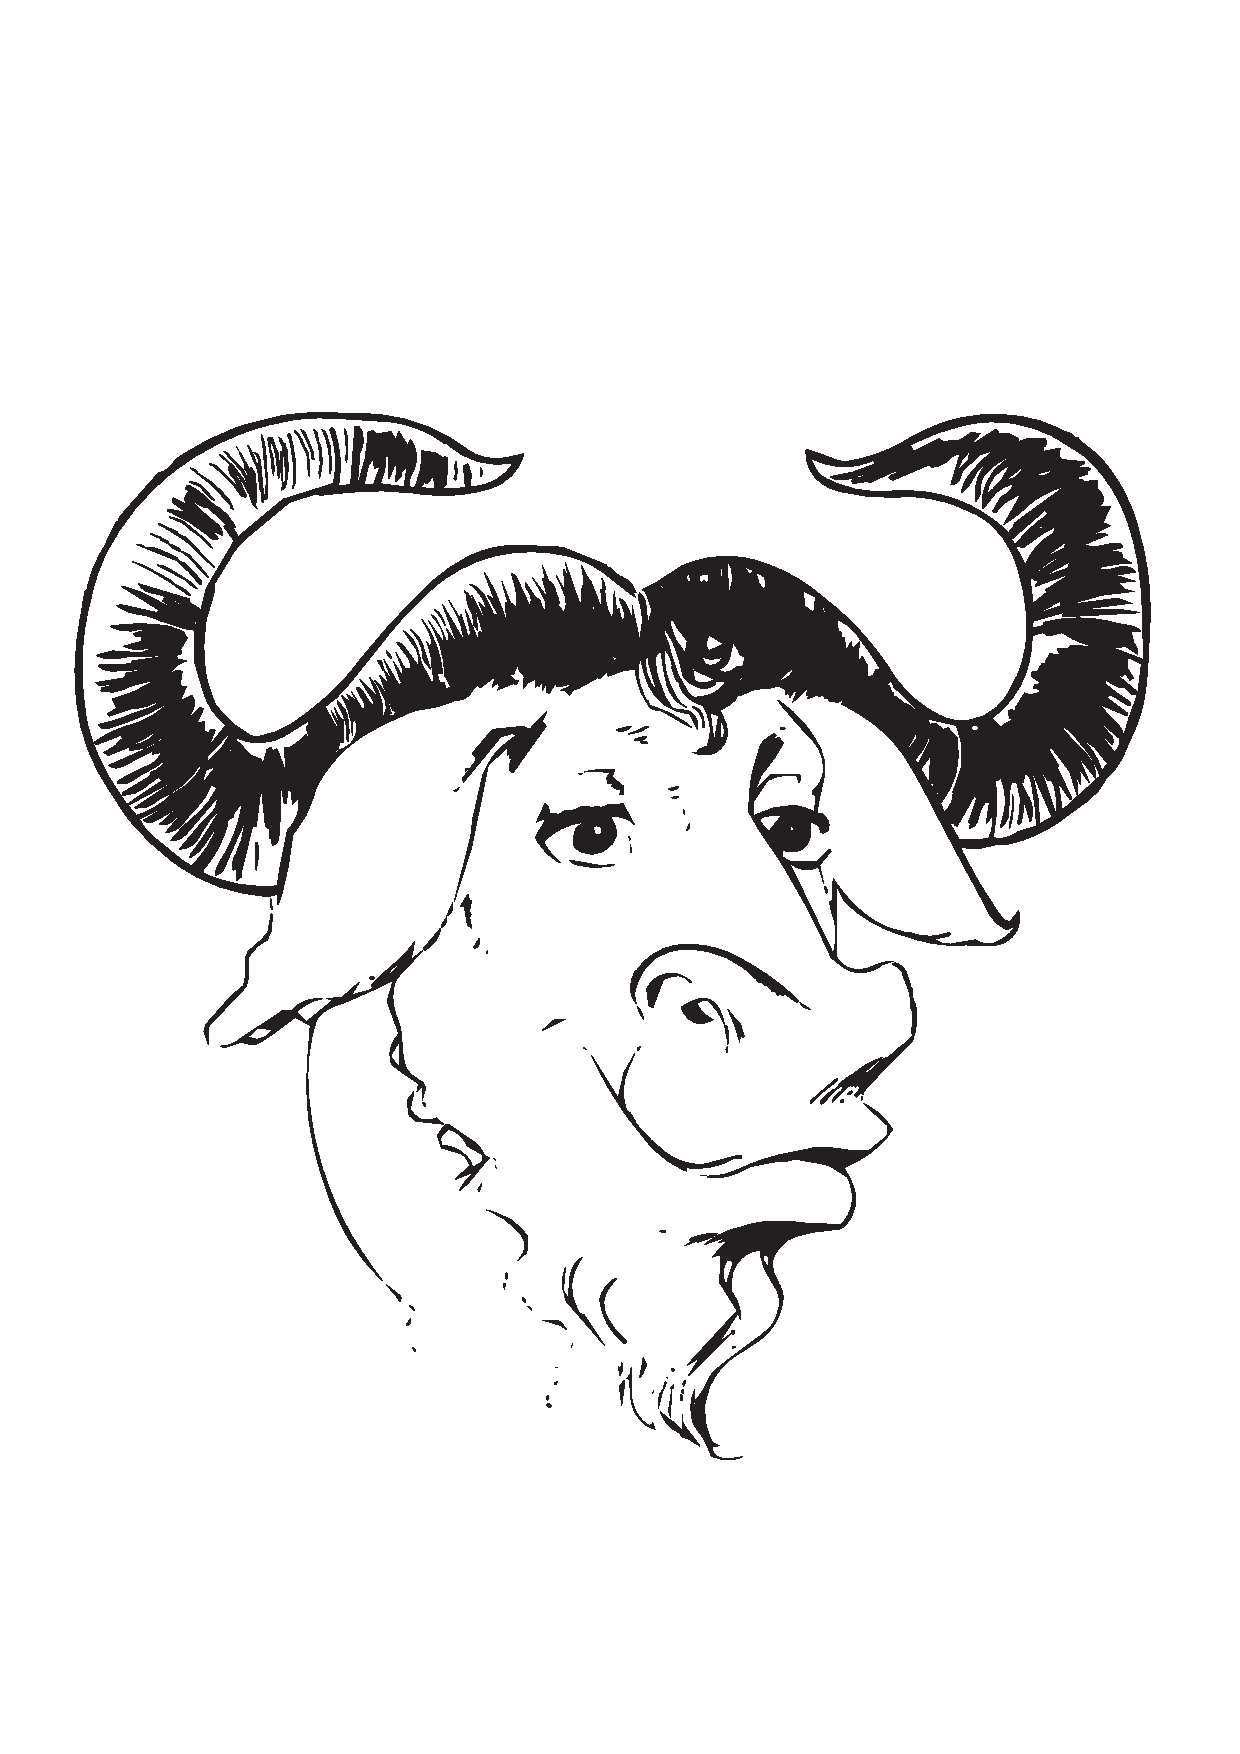
\includegraphics{images/gnu-head}}%
 \caption{\Y{labelfig} の使い方\label{fig:you}}%
\end{center} 
\end{figure} 
\end{InText}

\begin{figure}[htbp]
\begin{minipage}{.49\linewidth}
 \GridLineWidth{.2pt}
  \SetLabels 
  \T\L(.8*.45) 鼻\\
  \T\L(.2*.9) 左の角\\
  \T\L(.7*.9) 右の角\\ 
  \T\L(.75*.3)  口\\ 
  \T\L(.65*.1) 髭\\ 
  \T\L(.3*.6) 左目\\ 
  \T\L(.7*.6)  右目\\ 
  \endSetLabels
  \ShowGrid
  \strut\AffixLabels{%
    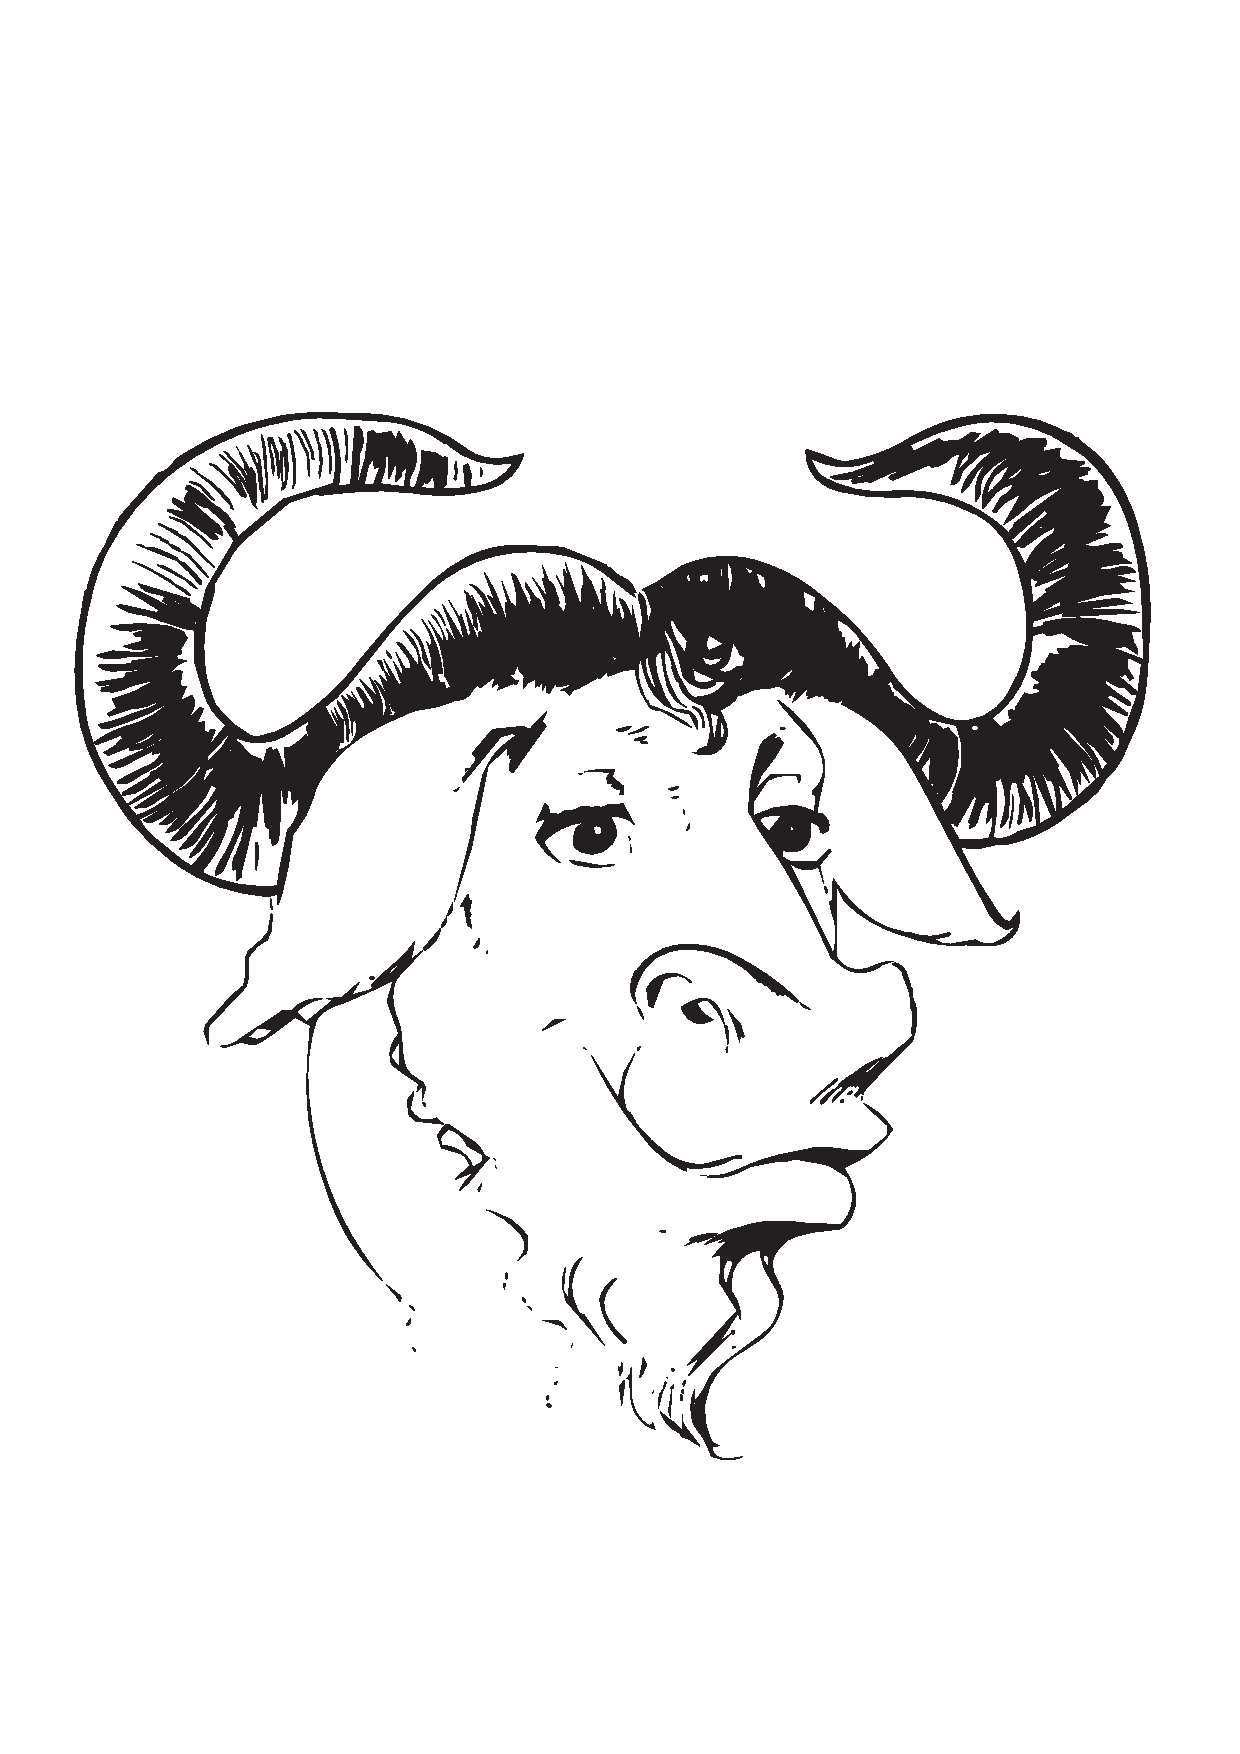
\includegraphics[clip,width=\linewidth]{images/gnu-head}}%
\end{minipage}
\hfil
\begin{minipage}{.49\linewidth}
  \SetLabels 
  \T\L(.8*.45) 鼻\\
  \T\L(.2*.9) 左の角\\
  \T\L(.7*.9) 右の角\\ 
  \T\L(.75*.3)  口\\ 
  \T\L(.65*.1) 髭\\ 
  \T\L(.3*.6) 左目\\ 
  \T\L(.7*.6)  右目\\ 
  \endSetLabels
  \strut\AffixLabels{%
    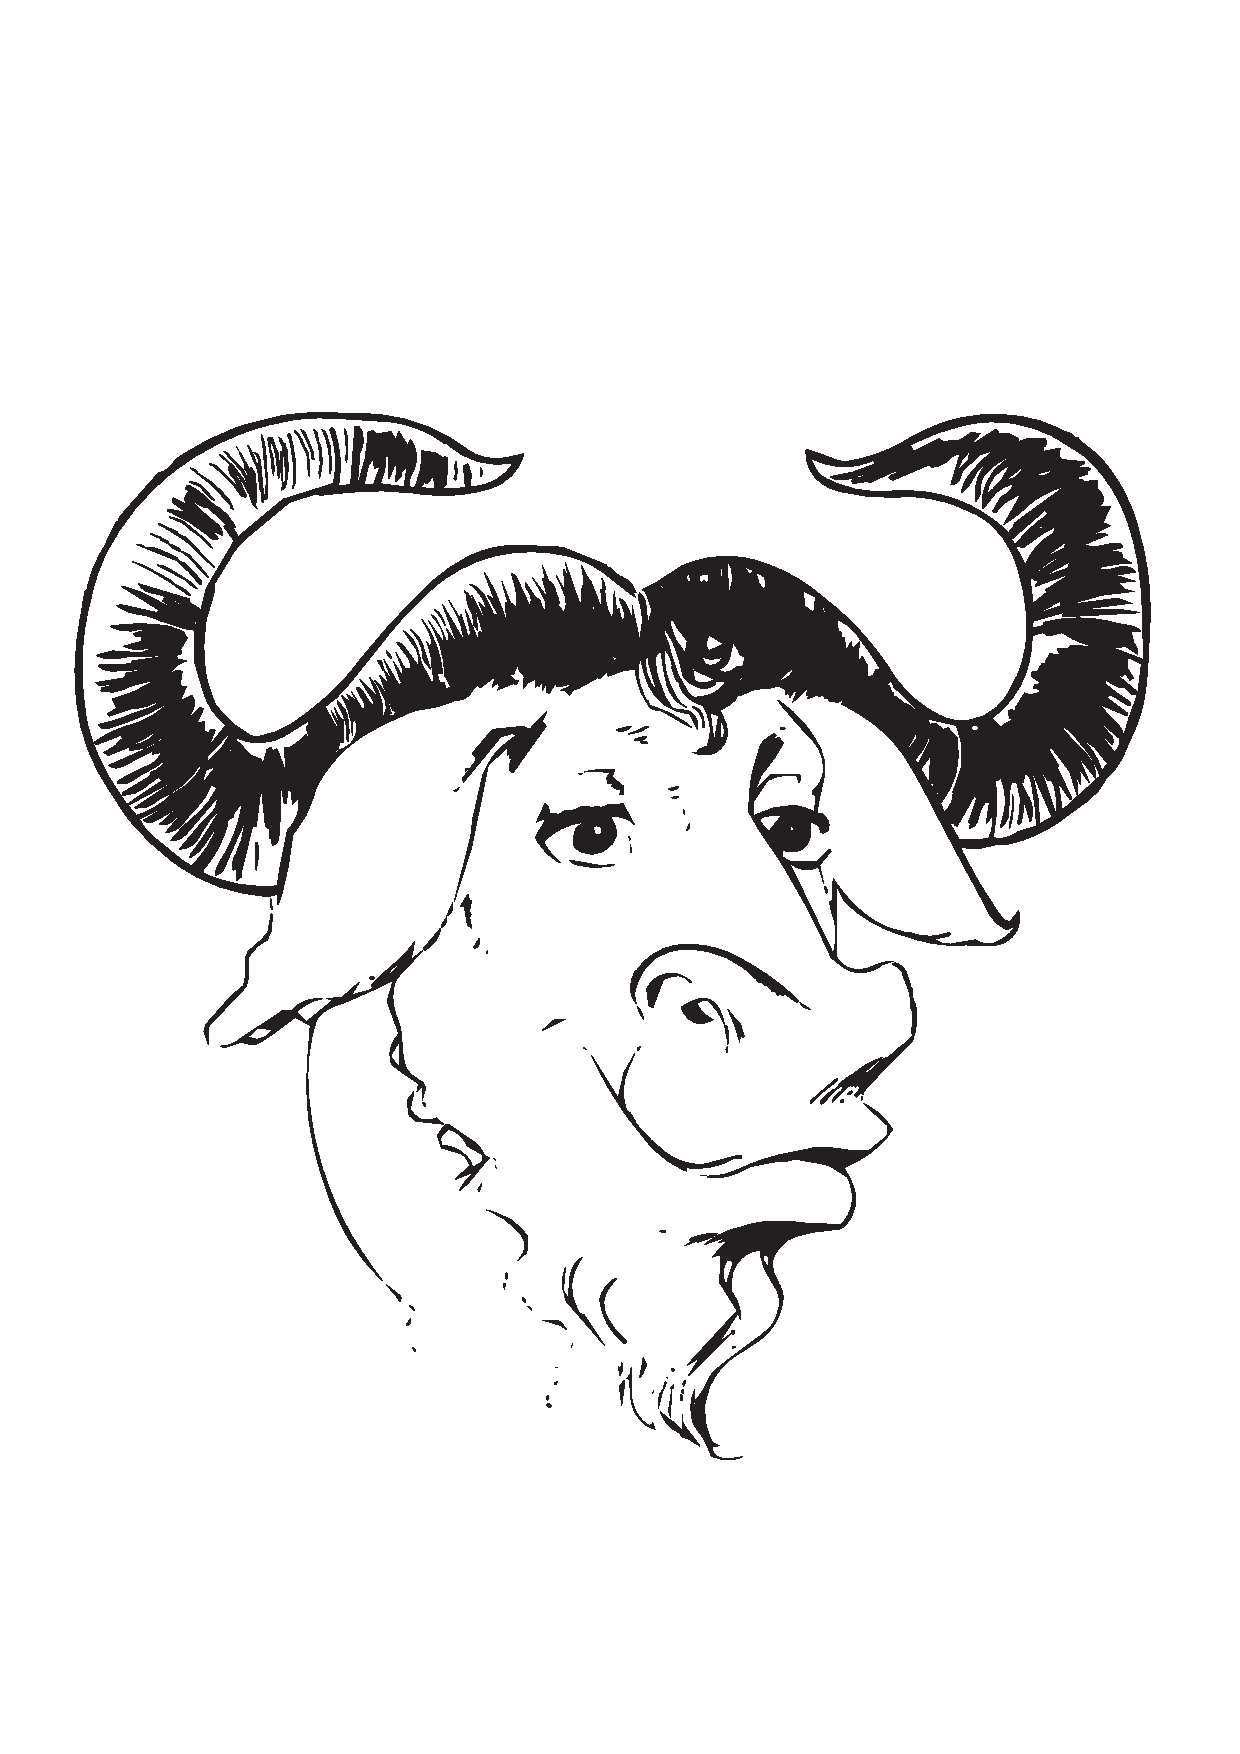
\includegraphics[clip,width=\linewidth]{images/gnu-head}}% 
\end{minipage}
 \caption{\sty{labelfig} の使い方\label{fig:labelfig}}%
\end{figure}


%レポートや論文などで図には\K{図見出し}を付けて\K{中央揃え}に
%するのが望ましいと思われますので
%\begin{InTeX}
%\begin{figure}[htbp]
% \begin{center}
%   \includegraphics[width=10cm]{images/file.eps}
%   \caption{図見出し}\figlab{samplefig}
% \end{center} 
%\end{figure} 
%\end{InTeX}
%のように使うことになるでしょう.ただし,これを毎回
%書くのは面倒なので次のような図用の\env{myfig}命令を
%作成します.
%\begin{InTeX}
%\newcommand{myfig}[4][width=.8\textwidth]{%
%\begin{figure}[htbp]%
%   \centering\includegraphics[#1]{#2}%
%   \caption{#3}\figlab{#4}%
%\end{figure}}
%\end{InTeX}
%このように定義しておけば次のように使えます.
%\begin{InTeX}
%以上の考察から図~\ref{fig:sample}のような
%図が得られる.
%\myfig[width=100pt,clip]{images/file.eps}{図の張り込みの例}{sample}
%\end{InTeX}


%浮動体の図はDVIファイルに出力されるときに思いも
%よらない場所まで旅をしますので,思い通りの場所に
%図を出力できなくても気にしないでください.
%そもそも図表に対して\yo{上記の図はなんちゃら}とか
%\yo{下記の図はなんちゃら}という表現は間違いで,
%全ての図表は\yo{図~3.1はなんちゃら}のように番号で
%参照します.ですから本来は図や表がどのような場所に
%旅立っても困らないはずです.

%図などを反時計回りに\kaku{90}回転させることがあるでしょう.
%その場合は \Cmd{rotatebox}命令を使います.
%他にも便利な命令があります.
%\begin{Syntax}
%\Cmd{rotatebox}\opa{設定}\pa{角度}{要素}
%\end{Syntax}
%これは \cmd{includegraphics}の任意引数に
%\qu{\str{angle}}を使ったことと同じです.
%\cmd{rotatebox}は図に限らずあらゆる要素を
%\Z{回転}します.\va{設定}の項目には以下のような
%ものがあります.
%\begin{description}
%\item[\str{origin=}\va{ラベル}] 
% 要素を回転するための原点を指定します.%%
% 左\qu{\str l},右\qu{\str r},中央\qu{\str c},
% 上部\qu{\str t},下部\qu{\str b}が指定できます.
%\item[\str{x=}\va{長さ}] 
%$x$方向の原点の位置を直接\va{長さ}を指定します.
%\item[\str{y=}\va{長さ}]
%$y$方向の原点の位置を直接\va{長さ}を指定します.
%\end{description}
%\indindz{回転}{文字列の}%%%
%\begin{InOut}
%\rotatebox{70}{文字列など}の
%\rotatebox[origin=c]{60}{回転とか}は
%\rotatebox[origin=b]{50}{どうよ?}
%\rotatebox{30}{だめぽ.}
%\end{InOut}

%要素を\K{拡大縮小}するには \cmd{scalebox}を
%使います.\index{拡大}\index{縮小}\indindz{拡大}{文字列の}
%\begin{Syntax}
%\Cmd{scalebox}\pa{横の拡大率}\opa{縦の拡大率}\pa{要素}
%\end{Syntax}
%\va{拡大率}には長さを指定します.\begin{InOut}
%\scalebox{2.3}{拡大縮小}\par
%\scalebox{3}[1]{拡大縮小}
%\end{InOut}
%
%要素の\K{反転}には \cmd{reflectbox}を使います.
%\begin{Syntax}
%\Cmd{reflectbox}\pa{要素}
%\end{Syntax}
%\begin{InOut}
%\reflectbox{文字列の反転}\par
%\reflectbox{山は山}\par
%\scalebox{-1}[1]{これも反転}
%\end{InOut}
%
%リサイズには \cmd{resizebox}を使います.
%\begin{Syntax}
%\Cmd{resizebox}\pa{幅}\pa{高さ}\pa{要素}
%\end{Syntax}
%要素のリサイズ後の幅を\va{幅}に,高さを\va{高さ}にします.
%どちらか一方の拡大・縮小率に合わせたいときは\qu{\str!}を
%使います.
%\begin{InOut}
%\resizebox{!}{1cm}{リサイズ}\par
%\resizebox{3cm}{!}{リサイズ}
%\end{InOut}

%以上の \cmd{rotatebox},\cmd{scalebox},\cmd{reflectbox},
%\cmd{resizebox}は文字列,表,図,\env{minipage}環境など
%の段落などにも使えます.\indindz{回転}{表の}%%
%\begin{InOut}
%\newcommand{\testtab}{\begin{tabular}{|c|}
%\hline \LaTeX\\ \LaTeXe \\ \hline %
%\end{tabular}}
%\rotatebox{80}{\testtab}~
%\reflectbox{\testtab}
%\end{InOut}


%\subsection{他のプログラムから張り込む方法その1}\seclab{excel:kowaza}
%例えば{Excel}や{PowerPoint}などのグラフや図表を張り
%込む場合大きく分けて次の3通りの方法があります.
%対象となるグラフや図表,ページは基本的にPS形式の
%画像に変換することができます.この小節の話はWindows
%に限定します.
%\begin{enumerate}
%\item 
% 該当のページなどをスクリーンショットでビットマップ画像と
% して保存しその画像を\Prog[EPSconv]{\EPSconv}や\Prog[ImageMagick]{\IM}
% でEPS画像に変換してから張り込む.
%\item 
%  ページなどの大きさを調整してから{\PS}プリンターを通して
%  プリンターファイルとして保存し,バウンディングボックスを
%  \Prog{eps2eps}で調整してから張り込む.
%\item 
%  ページなどの大きさをA4の紙いっぱいにファイルとして印刷し,
%  それを\textsf{graphicx}パッケージで回転と拡大・縮小をして張り込む.
%\end{enumerate}
%一つ目と二つ目は手間がかかるうえに印刷品質も悪いので
%ここでは説明しません.三つ目の方法を解説します.
%
%手順は以下の四つのようになります.MicrosoftのExcelの
%グラフを取り込む手順を例に出しています.
%\begin{enumerate}
%\item まず,{Windows}の\win{設定}で\win{プリンタの追加}をします.
%      追加するプリンタは\yo{ローカルプリンタ}で使用するポートは
%      \yo{ファイルへ出力}を選択し,ここでは\yo{HP Color Laser Jet PS}
%      というプリンタソフトウェアを選択します.テストページを印刷する
%      場合は,出力ファイル名を\qu{hoge.eps}のように拡張子を\exten{eps}にして
%      保存します.正しく印刷されいるかどうかを確認するには
%      \prog{\GS}か\prog{GSView}などで見ることができます.
%\item 次に元となるグラフやページを作成します.このとき
%      モノクロ印刷を想定してグラフを調整します.印刷したいグラフ
%      を選択したならば,\win{ページ設定}で印刷の向きは\yo{横},
%      用紙サイズは\yo{A4},\win{余白}タブで上下左右,ヘッダー,
%      フッターの余白をすべて\yo{0}に設定し,\win{ヘッダー,フッター}
%      タブで何も出力しないことを選択し,\win{グラフ}タブで,
%      印刷するグラフのサイズを\yo{用紙サイズ}に合わせます.
%      印刷品質は\yo{白黒印刷}にするとファイルサイズも小さくなり
%      処理速度も向上します.印刷プレビューで問題がないことを
%      確認したならば,{アプリケーション}側での設定は終了です.
%\item \win{ファイル}から\win{印刷}を選び,プリンタの名前を先程
%      追加したプリンタに設定します.\qu{OK}ボタンを押し絶対パスで
%      \zindind{ファイル}{に付ける名前}ファイル名を指定してファイルへ出力すれば,目的のグラフをEPS
%      で保存することができます.このとき保存するファイル名は半角
%      英数字とし拡張子は\exten{.eps}としてください.
%      ファイルの保存先を原稿と同じ場所にすると問題も少ないでしょう。
%\item 出力した\fl{filename.eps}を{\LaTeX}文書中で参照します.
%      \textsf{graphicx}パッケージを使って
%      \begin{quote}
%       \verb+\includegraphics[scale=0.4,angle=-90]{filename}+
%      \end{quote}
%      とすれば丁度良いあんばいで取り込めます.A4の紙に
%      グラフを出力した場合,0.4倍の縮小率で,時計回りに
%      90度回転させると{\LaTeX}文書の中で丁度良いサイズ
%      として張り込むことができます.
%\end{enumerate}
%以上の2--4の作業をグラフの数だけ繰り返すことにより,
%{\LaTeX}に対して{Excel}で作成されるグラフとほぼ同じイ%
%\indindz{フォント}{ビットマップ}\indindz{フォント}{ギザギザの}%%%
%メージを挿入することが可能です.フォントがビットマップ
%フォントでギザギザになるときはプリンタの設定で
%\yo{TrueTypeフォントダウンロードオプション}のような
%項目があるはずですので,これを\yo{アウトライン}にすると
%良いでしょう.


%\subsection{他のプログラムから取り込むとき}\seclab{picture:program}
%
%\Prog{Mathematica}や\Prog{Illustrator}からグラフや画像を取り込むときには
%幾つかコツが必要です.\secref{excel:kowaza}での{Excel}での張り込み方が他
%のアプリケーションでも適用できる場合が多いので,上記の方法を試してみてく
%ださい.
%
%どのプログラムを使用していても最終的に出力したい画像のサイズを元のプログ
%ラム側で調節してから{\LaTeX}に張り込むようにすると問題も少ないでしょう.
%\sty{graphicx}パッケージの拡大縮小を使うと印刷品質が落ちます.各プロ
%グラムにおける設定方法は以下の通りです.
%\begin{description}
%\item[\prog{Illustrator}]
% まず文字はアウトライン化します.
% ツールバーの\win{別名で保存}でファイル形式を\qu{Illustrator
% EPS}として保存します.EPS形式での保存オプションで\yo{サムネー
% ルを作成}の\K{チェックを外して},\yo{フォントデータを含む}
% のチェックをはずしてください.ポストスクリプトのレベルは\qu{{\PS} 
% level 2}としてください.プレビューについては\qu{8-bit IBM PC}で良い
% と思います.{Illustrator}の場合はサイズが自動的に調節されますの
% で用紙サイズを設定する必要はありません.
%誤ってサムネールを付けた場合バージョンによってエラーに
%なるので\Person{Tomas}{Rokicki}の\Prog{fixill.pl}を使うと
%良いでしょう.Perlスクリプトで書かれており,実行するためには
%Perlが必須で
%\begin{InTerm}
%   \type{fixill < input.eps > output.eps}
%\end{InTerm}
%のように使います.
%
%\item[\Prog{photoshop} ver.7]
%\win{ファイル},\win{複製を保存}を選び\yo{保存形式}
%を\qu{Photoshop EPS}にして保存する.保存オプション
%で\yo{エンコーディング}は\qu{ASCII}とする.ビッ
%トマップ画像はエンコーディングで圧縮しないほうが
%印刷品質が良いでしょう.
%
%\item[\Prog{Mathematica} ver.4]
%ツールバーから\win{ファイル}の\win{特殊な形式で保存}を選び
%\win{TeX(X)}を選びます. そうすると数式やグラフなどが自動的に
%{\LaTeXe}形式に保存されます.またグラフはEPS形式で{\fl{
%filename.eps}}という名前で保存されます.{Mathematica}の場合
%出力されるEPS画像の\Z{バウンディングボックス}が正常に
%出力されないことがあるので{\LaTeX}で正しく処理できない場合
%があります.出力された\fl{filename.eps}というファイルを
%テキストエディタで開けば
%\begin{InText}
%%%BoundingBox: 91.5625 3.1875 321.938 190
%\end{InText}
%のような記述があります.これは画像を平面上
%のどこに配置するかを指定するもので,左から
%2次元平面上の始点の$x_0$と$y_0$,終点の$x$と
%$y$に対応します.また,通常はこの値は整数値が
%推奨されます.上記の数値を四捨五入して整数に
%直して取り込んでください.
%
%\item[\Prog{MATLAB}]%underfull
%グラフを表示しているMATLABプログラムのウィンドウの
%ツールバーにある\win{ファイル}から\win{エクスポート}を
%選び,ファイルの種類を\qu{EPS Level 2}にし,任意の名前
%をつけて保存します.{Illustrator}形式での出力もサポート
%されていますので,お持ちの場合はグラフを編集できるのでは
%ないでしょうか.
%
%%\item[{Gnuplot}]
%%{Gnuplot}については\pref{subsec:gnuplot}
%%\secref{subsec:gnuplot}で詳しく解説してあります.
%\end{description}
%
%%他のプログラムから取り込むならば{\LaTeX}側である程度
%%対応できますが,{\LaTeX}で作成したページや数式を
%%Illustratorに持っていって,それを加工した図を作成する
%%という場合は{\LaTeX}の出力をアウトライン化すると
%%うまくいきます.{\LaTeX}で使われているフォントは
%%\Person{Donald}{Knuth}氏のデザインしたComputer Modernフォント
%%などが使われていることが多いのですが,それらが各OSの
%%システムにインストールされていないと不明なフォントとして
%%代替フォントに置き換わったりします.システムに{\LaTeX}
%%のフォントをインストールできればそれでよいのですが,
%%できない場合を考えてみたいと思います.
%
%%platex input
%%dvips -Ppdf -E  -o input.eps input
%%eps2eps input.eps output.eps
%
%
%\subsection{図を二つ横に並べる}
%2段組の場合はそのようなことはありませんが,
%1段組の場合は一つの図だけでは両脇が開いてしまうので
%そこに二つの図を\qu{(a)}と\qu{(b)}として挿入したい
%ときがあります.このようなときは\Env{minipage}環境
%を使います.以下のように入力する例もあります.
%\begin{InTeX}
%\begin{figure}[htbp]
%  \begin{minipage}{.47\textwidth}
%      \centering%ここに図(a)を入れる
%      (a) 初期値$c=0.6$
%  \end{minipage}
%\hfill
%  \begin{minipage}{.47\textwidth}
%      \centering%ここに図(b)を入れる
%      (b) 初期値$c=1.0$
%  \end{minipage}
%  \caption{1段組で横に図を二つ並べる}
%\end{figure}
%\end{InTeX}
%両方の図の番号を別にしたいときも同様に
%記述します.
%
%%方向性が若干異なりますが,図の隣に文字列を並べる
%%のも同様の方法でできるわけです.
%%\begin{wrapfigure}{r}{5cm}
%%
\includegraphics[bb=0 0 124 98,clip]{images/vector}
%%\end{wrapfigure}
%%例として\Person{Donald}{Arseneau}による\Sty{wrapfig}
%%を使う場合をご覧ください.このような出力を得るために
%%\begin{InTeX}
%% \begin{wrapfigure}[5]{r}{5cm}
%% \includegraphics{file}
%% \end{wrapfigure}
%%\end{InTeX}
%%という入力をします.
%




%\begin{Syntax}
% \C{DeclareGraphicsExtensions}\pa{拡張子のリスト}\\
% \C{DecrelaGraphicsRule}\pa{拡張子}\pa{種類}\pa{読み込むファイル}\pa{コ
% マンド}
%\end{Syntax}

%\subsection{EPS以外の画像の張り込み}
%{\LaTeX}ではEPS以外の画像の張り込みも可能
%ですが少々癖があります.お手元にはGIFやBMP,
%JPEGなどのビットマップ画像があると思います.
%ビットマップ画像をEPSに変換できるツールは
%無料でたくさんあり,有名なのが\prog{\IM}
%です.{Windows}専用ですが\Prog[EPSconv]{\EPSconv}\footnote{\webEpsconv}
%というソフトウェアを導入することにより,
%現存するほとんどの画像をEPSに変換可能です.
%これらのアプリケーションはあくまでビットマップ
%をEPS形式で保存するだけなのでファイルサイズが非
%常に大きくなります.
%
%デバイスドライバとして\prog{\Dvipdfmx}を使うと
%EPS形式以外の画像でも取り込むことができます.
%%本来ならばBMPやJPG形式は{\EPSconv}や{\IM}などの
%%ツールを使って一度EPSに変換する手順が必要でした
%%が\prog{\Dvipdfmx}の場合はその手順が必要ありません.
%変換しなくても取り込める形式はPDF,JPEG,PNG,MetaPostの4種類
%です.{Windows}のBMPなどは低圧縮のJPEGなどに
%変換します.\fl{image.png} があった場合
%端末などで
%\begin{InTerm}
%   \type{ebb image.png}
%\end{InTerm}
%とすれば\fl{image.png}用の\fl{image.bb}が
%作成されます.\prog{ebb}は{dvipdfm}に
%同封されています.この\texttt{image.bb}は
%画像ファイルの縦横を正しく扱うためのフ
%ァイルです.\texttt{image.bb} を見れば
%分かりますが,中身は
%\begin{InText}
%%%Title: ./image.png
%%%Creator: ebb Version 0.5.2
%%%BoundingBox: 0 0 595 841
%\end{InText}
%となっています. \qu{\str{BoundingBox}}とは
%原点座標と画像の縦横の長さの値です.
%次にソースファイルを以下のようにします.
%\begin{InTeX}
%\documentclass{jsarticle}
%\usepackage[dvipdfm]{graphicx}
%\begin{document}
%\includegraphics[width=3cm]{image.png}
%\end{document}
%\end{InTeX}
%後はいつも通りにタイプセットしてDVIファイルを
%生成し\prog{\Dvipdfmx}でPDFを作成すれば良いこ
%とになります.
%
%\subsection{EPSからPDFへの変換}
%デバイスドライバとして\prog{\Dvipdfmx}で手持ちの
%EPS画像を取り込むようにしている場合,\prog{\Dvipdfmx}
%を実行するたびに毎回\Prog[Ghostscript]{\GS}を使ってEPSからPDFに変換
%する処理が行われます.処理時間の短縮のために,
%あらかじめPDFに変換しておけば良いでしょう.EPS形式
%の画像をPDFへ変換する方法はいくつかあるそうですが,
%簡単で安全な方法を紹介します.まず\prog{\GS}の
%\qu{pdfwrite}の力を借りる方法です.BoundingBoxの
%設定されているEPS画像を\Prog{epstopdf}によって
%PDFに変換します.
%\begin{InTerm}
%   \type{epstopdf filename.eps}
%\end{InTerm}
%とすると\fl{filename.pdf}が作成されます.日本語が
%使われているEPSがうまく処理できないなどの
%問題があるかもしれません.その場合はGNUの
%\Prog[GhostScript]{\GS}のバージョン7.07を使うと良いで
%しょう.以下のようなシェルスクリプト\fl{epspdf}
%\begin{InText}
%#!/bin/bash
%FILE=$1
%fig=`basename $FILE .eps`
%epstopdf $FILE
%egrep "%%BoundingBox:" $FILE > $fig.bb
%\end{InText}
%を作成し\fl{/usr/local/bin/}などに複製して%$
%\begin{InTerm}
%   \type{epspdf filename.eps}
%\end{InTerm}
%とするとPDFファイル\fl{filename.pdf}とバウンデ\indindz{ファイル}{PDF}%
%ィングボックス情報\fl{filename.bb}が作成されま
%す.%\prog{echo}は端末に文字を出力する命令,
%%\prog{test}は文字列を検査する命令,
%%\prog{egrep}はファイルなどから特定の表現を見つける命令,
%%\prog{basename}はファイル名から拡張子を取り除いたりする命令.
%同じディレクトリの中の全てのEPS画像を
%PDFに変換したいときは
%\begin{InText}
%#!/bin/sh
%for f in `ls *.eps`; do
%   fig=`basename $f .eps`
%   epstopdf $f
%   grep "^%%BoundingBox:" $f > $fig.bb
%done
%\end{InText}
%を\fl{epspdfs}という名前で同じように複製します.
%このようにして処理したPDFは{\LaTeX}の原稿で
%\begin{InTeX}
%\documentclass{jsarticle} 
%\usepackage[dvipdfm]{graphicx}
%\begin{document}
%\includegraphics{filename.pdf}
%\end{document}
%\end{InTeX}
%のようにして取り込むことができます.
%
%\begin{comment}
%ちなみに\fl{filename.bb}は
%\begin{InText}
%%%Title: filename.dvi
%%%Creator: hoge
%%%BoundingBox: 142 160 443 665
%%%CreationDate: Tue Dec 30 16:01:48 2003
%\end{InText}
%のような情報が出力されているでしょう.この中の
%\begin{InText}
%%%BoundingBox: 142 160 443 665 
%\end{InText}
%という1行だけあれば,\prog{\Dvipdfmx}等は画像を
%張り込むことができます.
%%%以上のようなシェルスクリプトを動作させることができないWindowsユーザの
%%%方はフリーのCygwinを導入されるのが良いと思うのですが\verb|^^;|.
%\end{comment}

\section{描画の方法}
{\LaTeX}で図を取り扱う手段はいくつも存在します.
写真のような画像を\sty{graphicx}パッケージ
などを使って張り込む方法と,1から描画する方法です.
\sty{graphicx}パッケージを用いて既存の画像を張り込む
方法は\secref{figure}を参照してください.画像を
まだ作成していない段階での描画の方法を紹介します.

描画の方法は大きく分けて二つあります.一つは{\LaTeX}
自身の能力で描画する方法と \cmd{special}命令を使い
他のプログラム(デバイスドライバ等)へ描画をゆだねる方法です.一般に
{\LaTeX}における描画の能力は{\TeX}譲りのシステムの
お陰で貧弱なものとなっています.簡単な図を作成する
ならば{\LaTeX}に備わっている\env{picture}環境に
よる描画を行うのが手軽です.

\subsection{べた書きによる図の作成}
もっとも簡単な描画の方法として{\LaTeX}でべた書きを
行う,\Env{verbatim}環境を使う事が考えられます.
\env{verbatim}環境内では文字が{\KY{等幅}}に近い字詰めで
組まれるので,原稿で入力している表示とDVIファイル
への出力が同じようになります%
\footnote{\Hito{内田}{昭宏}の作成した\Prog{plain2}というツールを使うと全
角記号を組み合わせる事によって{\LaTeX}用の図表を作成することもできます.}.

\begin{Exe}
以下の入出力例を参考にべた書きによる作図をしてみてください.
\begin{InOut}
\begin{verbatim}
       a
      /  \
     /    \
    b      c
   / \    / \
  d   e  f   g
\end{verbatim}
\end{InOut}

%\env{verbatim}環境内では半角の空白を使わずに
%全角の空白を使うと良いでしょう.半角の空白は
%テキストエディッタで入力している分の空白が
%挿入されるわけではありません.
\end{Exe}




\subsection{曲
  線の描画}
\indindz{曲線}{スプライン}\indindz{曲線}{近似}\indindz{曲線}{ベジェ}%
{\KY{ベクトル画像}}などでは{\KY{ベジェ曲線}}
とか{\KY{スプライン曲線}}という{\KY{近似曲線}}
が使われていると多くの参考書で記述されています.ベクトル画像を
知るうえでベジェ曲線の原理を知っておくと,曲線を描くと
きに頭の中で曲線をイメージしやすいと思いますので紹介
しておきます.滑らかな曲線を描くためには多くの点座標
が必要になると思う人もいるでしょうが,ある程度滑らか
な曲線を描くためには3点あれば十分です.\indindz{点}{制御}
曲線を描くための点\pp{\Z{制御点}}が少なければ少ないほど情報
量は少なくなるので,少ない制御点で滑らかな曲線を描く
方法が過去に模索されました.その中でもベジェ曲線は高
々二つの基準点と一つの制御点\pp{$2+1$点}があれば現在私
たちが\prog{Illustrator}などでよく見かける曲線になり
ます.この原理が\Prog{Illustrator}のペンツールに活か
されていますので,お持ちの方は確認していただくと良いで
しょう.ただ\Prog{Illustrator}の場合はユーザの見えな
い箇所で様々な工夫がなされています.

曲線を描くためにいま$n$個の制御点がありその$i$番目
の座標を$P_i=(x_i,y_i)$として\equref{bez1}と
\equref{bez2}で表す曲線をベジェ曲線と呼びます.
\begin{eqnarray}
P(u)&=&\sum^{n-1}_{i=0} P_i\, B_{i, n} (u)\equlab{bez1}\\
B(u)&=&\frac{n!}{i!\, (n-i)!}u^i(1-u)^{n-i}\equlab{bez2}
\end{eqnarray}
\indindz{フォント}{Type1}%%
これがベジェ曲線の一般形ですが,例としてType1フォントで
も使われている?2次ベジェ曲線を示します.
平面座標に$P_0=(-1,1)$,$P_1=(0,0)$,$P_2=(1,1)$が
あるとすれば\equref{bez1}と\equref{bez2}より,
\begin{eqnarray}
 P(u)&=& P_0 B_{0,2} + P_1 B_{1,2} + P_1 B_{1,2} \nonumber\\
     &=& P_0 (1-u)^2 + P_12u(1-u) + P_2 u^2 \equlab{bez3}
\end{eqnarray}
となり\equref{bez3}に対して無数の$u$を与え
れば滑らかな曲線を描けます.これは3次元でも同
様に計算できるので便利な式です.例の基準点,制御点と
ベジェ曲線は\figref{bez1}の通りになります.
\begin{figure}[htbp]
\begin{center}
\setlength{\unitlength}{1cm}
\begin{picture}(6,4)(0,0)
 \put(0,2){\vector(1,0){6}}
 \put(6.2,2){\makebox(0,0)[b]{$x$}}
 \put(3,0){\vector(0,1){4}}
 \put(3.2,4){\makebox(0,0)[t]{$y$}}
 \multiput(0,1.9)(1,0){6}{\line(0,1){.2}}
 \multiput(2.9,0)(0,1){4}{\line(1,0){.2}}
 \put(2,3){\circle{.1}}
 \put(2,3.1){\makebox(0,0)[b]{$P_0$}}
 \dashline{.1}(2,3)(3,2)
 \put(3,2){\circle{.1}}
 \put(2.8,1.9){\makebox(0,0)[t]{$P_1$}}
 \put(3.2,1.9){\makebox(0,0)[t]{$O$}}
 \put(4,3){\circle{.1}}
 \put(4,3.1){\makebox(0,0)[b]{$P_2$}}
 \dashline{.1}(4,3)(3,2)
 \qbezier(2,3)(3,2)(4,3)
\end{picture}
\caption{制御点と式から得られるベジェ曲線}\figlab{bez1}
\end{center}
\end{figure}
このような原理を知っておくと後ほど紹介する
{\LaTeX}の\env{picture}環境で使用できる命令の
理解に役立つ事でしょう.ただし{\LaTeX}
での多くのベジェ曲線を描くコマンドはもっと
計算の少ないアルゴリズムを使っている場合が
ありますし,デバイスドライバに描画を任せている
事もあります.


\subsection{\env{picture}環境による描画}
{\LaTeX}の力を使った描画を行うには特別な環境,
描画専用の\Env{picture}環境で作業を使います.
\env{picture}環境では基準となる長さを決めてその
相対的な距離によって描画を行います.このとき基準
となる長さ \cmd{unitlength}を決めます.
\begin{Syntax}
\verb+\begin{picture}+\xy{x}{y}\xy{$x_0$}{$y_0$}\\
\va{描画内容}\\
\verb+\end{picture}+
\end{Syntax}
\env{picture}環境の中に描画したい内容を
記述します.\env{picture}環境に渡す\qu{\xy{x}{y}}
は必須引数ですが\qu{\xy{$x_0$}{$y_0$}}は任意引数です.
\qu{\xy{x}{y}}には座標における\env{picture}環境の大きさ
を横方向は$x$で縦方向は$y$で指定します.
これには単位などを付けずに数値で指定します.
\qu{\xy{$x_0$}{$y_0$}}には原点の位置を指定します.

何らかの要素を配置するには \cmd{put}か \cmd{multiput}を
使います.$x$と$y$は単位 \cmd{unitlength}に
従属します.
\begin{Syntax}
\Cmd{put}\xy{x}{y}\pa{要素}\\
\Cmd{multiput}\xy{x}{y}\xy{$\Delta{x}$}{$\Delta{y}$}%
  \pa{回数}\pa{要素}
\end{Syntax}
\cmd{put}命令は座標\xy{x}{y}に\va{要素}を置くだけの
命令です.\cmd{multiput}は座標\xy{x}{y}を基点とし,
二つ目の座標\xy{$\Delta{x}$}{$\Delta{y}$}を\Z{ベクトル}
として\xy{$\Delta x$}{$\Delta y$}の変化量に応じて
要素を回数分だけ繰り返して配置します.
この他に2次ベジェ曲線を描く \Cmd{qbezier}命令があります.\zindind{曲線}{の描画}
\begin{Syntax}
\Cmd{qbezier}\xy{$x_1$}{$y_1$}\xy{$x_2$}{$y_2$}\xy{$x_3$}{$y_3$}
\end{Syntax}
\qu{\xy{$x_1$}{$y_1$}}を始点,\qu{\xy{$x_2$}{$y_2$}}
を基準点,\qu{\xy{$x_3$}{$y_3$}}を終点として2次ベジェ
曲線を描きます.

\va{要素}には次のようなコマンドが標準として使えます.
\begin{Syntax}
\Cmd{line}\xy{x}{y}\pa{長さ}\\
\Cmd{vector}\xy{x}{y}\pa{長さ}\\
\Cmd{circle*}\pa{直径}\\
\Cmd{oval}\xy{幅}{高さ}\opa{位置指定}
\end{Syntax}
\cmd{line}は\qu{\xy{x}{y}}をベクトルとして
\va{長さ}分の線分を描きます.\cmd{vector}は \cmd{line}
の終端に\Z{矢印}をつけたものです.
\cmd{circle*}は直径を指定して\Z{円}を描きます.\indindz{描画}{円の}%
アスタリスク\qu{\texttt*}を付けないと円の内側が塗りつぶされません.
\cmd{oval}は幅と高さを指定して楕円を描きます.\indindz{描画}{楕円の}%
\begin{InOut}
\setlength{\unitlength}{1mm}
\begin{picture}(40,30)
\put(10,10){\line(1,1){10}}
\put(10,0){\vector(1,1){10}}
\put(20,20){\circle{5}}
\end{picture} 
\end{InOut}
楕円を描く \cmd{oval}命令の任意引数の\va{位置指定}
には楕円のどの部分を出力するかを指定します.
それぞれ上部\qu{\str t},下部\qu{\str b},
左\qu{\str l},右\qu{\str r}となり,複合的に
使用できます.
\begin{InOut}
\setlength{\unitlength}{1mm}
\begin{picture}(50,30)
\put(8,12){\oval(10,15)[tl]}
\put(8,8){\oval(10,15)[bl]}
\put(10,10){\oval(10,15)}
\put(12,12){\oval(10,15)[tr]}
\put(12,8){\oval(10,15)[br]}
\end{picture} 
\end{InOut}
\env{picture}環境中での線の太さは
\Cmd{thinlines}と \Cmd{thicklines}の二つで調整
します.\cmd{thinilnes}のほうが細く \cmd{thicklines}
のほうが太くなります.\env{picture}環境中の全て
の線分に有効になります.
\begin{InOut}
\setlength{\unitlength}{1mm}
\begin{picture}(50,30)
\thicklines
\put(10,10){\line(1,1){10}}
\put(10,20){\vector(1,1){10}}
\thinlines
\put(10,0){\vector(1,1){10}}
\put(20,20){\circle{5}}
\end{picture}  
\end{InOut}

\begin{Exe}
\figref{bez1}を \env{picture} 環境で描画するにはどうすれば
良いかを考えてください.例を示すと以下のような記述になります.

\C*{makebox}%
\begin{InTeX}
\setlength{\unitlength}{1cm}
\begin{picture}(6,4)(0,0)
 \put(0,2){\vector(1,0){6}}
 \put(6.2,2){\makebox(0,0)[b]{$x$}}
 \put(3,0){\vector(0,1){4}}
 \put(3.2,4){\makebox(0,0)[t]{$y$}}
 \multiput(0,1.9)(1,0){6}{\line(0,1){.2}}%後述
 \multiput(2.9,0)(0,1){4}{\line(1,0){.2}}%後述
 \put(2,3){\circle*{.1}}
 \put(2,3.1){\makebox(0,0)[b]{$P_0$}}
 \dashline{.1}(2,3)(3,2)%後述
 \put(3,2){\circle*{.1}}
 \put(2.8,1.9){\makebox(0,0)[t]{$P_1$}}
 \put(3.2,1.9){\makebox(0,0)[t]{$O$}}
 \put(4,3){\circle*{.1}}
 \put(4,3.1){\makebox(0,0)[b]{$P_2$}}
 \dashline{.1}(4,3)(3,2)%後述
 \qbezier(2,3)(3,2)(4,3)
\end{picture}
\end{InTeX}

\end{Exe}

\subsection{\env{picture}環境の拡張その1\zdash \sty{epic}}
{\LaTeX}での標準の\env{picture}環境のコマンドも
デバイスに依存しないので汎用性があるのですが,
それではあまりにも表現力に乏しいのが現状です.
そこでこの\env{picture}環境の拡張が行われて
きました.\env{picture}環境に限らず{\LaTeX}での描画
は1980年代後半からさまざまな方法が模索され,拡張
され続けました.その中でも\Person{Sunil}{Podar}による
\Sty{epic}は\env{picture}環境の拡張版としては定評が
あります.\sty{epic}では{\LaTeX}の\env{picture}環境
で使用できるコマンドのほかに以下の命令が拡張されています.
\begin{quote}% underfull
\begin{tabular}{lllll}
\Cmd{multiputlist}&\Cmd{matrixput}&\Cmd{grid}&\Cmd{picsquare}&\Cmd{dottedline}\\
\Cmd{dashline}&\Cmd{drawline}&\Cmd{jput}&\Cmd{putfile}& \\
\end{tabular}


\end{quote}
このほかに\Env{dottedjoin},\Env{dashjoin},\Env{drawjoin}の
三つの環境が定義されています.
座標の変化量を\xy{$\Delta{x}$}{$\Delta{y}$}として複数の
項目を配置する \cmd{multiputlist}命令があります.
\begin{Syntax}
\Cmd{multiputlist}\xy{x}{y}\xy{$\Delta{x}$}{$\Delta{y}$}%
   \opa{tbrl}\pa{複数の項目}
\end{Syntax}
% tbrl のいずれかを指定します.
座標上に行列のように要素を繰り返して配置する \cmd{matrixput}命令もあります.
\begin{Syntax}
\Cmd{matrixput}\xy{x}{y}\xy{$\Delta{x_1}$}{$\Delta{y_1}$}%
   \pa{$n_1$}\xy{$\Delta{x_2}$}{$\Delta{y_2}$}%
   \pa{$n_2$}\pa{要素}
\end{Syntax}
\begin{InOut}
\setlength{\unitlength}{1pt}
\begin{picture}(150,110)(0,0)
\multiputlist(0,0)(15,10)%
  {0,1,2,3,4,5,6,7,8,9,10}
\matrixput(0,0)(20,0){7}(0,20)%
   {5}{\mbox{未来}}
\end{picture} 
\end{InOut}
座標系を表現するのに格子を描くには \cmd{grid}命令が使えます.
\begin{Syntax}
\Cmd{grid}\xy{幅}{高さ}\xy{$\Delta{\text{幅}}$}{$\Delta{\text{高さ}}$}%
   \opa{$x$座標の初期値,$y$座標の初期値}
\end{Syntax}
%\begin{InOut}
%\begin{picture}(150,100)(0,0)
%\put(10,10){\grid(50,50)(10,10)[0,0]}
%\end{picture} 
%\end{InOut}
\indindz{描画}{折れ線の}\indindz{描画}{破線の}\indindz{描画}{点線の}%%
他にも点線や破線などを描くコマンドがあります.
\begin{Syntax}
\Cmd{dottedline}\opa{点の種類}\pa{間隔}%
   \xy{$x_1$}{$y_1$}\xy{$x_2$}{$y_2$}$\cdots$\xy{$x_n$}{$y_n$}\\
\Cmd{dashline}\pa{破線の長さ}\opa{間隔}%
   \xy{$x_1$}{$y_1$}\xy{$x_2$}{$y_2$}$\cdots$\xy{$x_n$}{$y_n$}\\
\Cmd{drawline}\xy{$x_1$}{$y_1$}\xy{$x_2$}{$y_2$}$\cdots$\xy{$x_n$}{$y_n$}
\end{Syntax}
\cmd{dottedline}は点線を,\cmd{dashline}は破線を,
\cmd{drawline}は\Z{折れ線}を描くために使います.\Z{点線}や\Z{破線}は
折れても構いません.
\begin{InOut}
\setlength{\unitlength}{1pt}
\begin{picture}(150,120)(0,0)
\put(0,0){%
  \grid(100,100)(25,25)[0,0]}
\dottedline[$\circ$]{10}(0,0)
  (100,100)
\dashline{3}(0,80)(30,50)(50,45)
  (100,20)
\drawline(0,70)(10,60)(30,40)
  (100,50)
\end{picture} 
\end{InOut}

\subsection{\env{picture}環境の拡張その2\zdash \sty{eepic}}
\Person{Sunil}{Podar}による\Sty{epic}を改良・拡張したものとして,
\Person{Conrad}{Kwok}の作成した\Sty{eepic}があります.これは\sty{epic}の
改良・拡張版でありますので使用するときは次のように\sty{epic}も先に読み込
んでおきます.

\begin{InTeX}
\usepackage{epic,eepic} 
\end{InTeX}

{\LaTeX}の\env{picture}環境で使用できる \cmd{line},
\cmd{circle*},\cmd{oval}の拡張が行われています.
\sty{epic}のコマンドも全て再定義されています.
\sty{eepic}はこれらの命令を{\Tpic}スペシャルに置き換え
ていますので描画力は高いのですが,デバイスドライバが
{\Tpic}スペシャルに対応している必要があります.
\prog{dviout},\prog{dvips},\prog{\Dvipdfmx}などは
対応しているようです.デバイスドライバによって{\Tpic} 
スペシャルの解釈が若干異なるようですので,出力を確認して
デバイスを選択してください.

線の太さに関するコマンドが新たに定義されています.
\begin{Syntax}
\Cmd{allinethickness}\pa{太さ} \\
\Cmd{Thicklines}
\end{Syntax}
\cmd{allinethickness}はこの命令を使った後の
\env{picture}環境中にある全ての線の太さを変更します.
\Cmd{Thicklines}は \Cmd{thicklines}よりもこのコマンドを
宣言した後の線の太さを太くします.
\setlength\unitlength{1pt}
\begin{InOut}
\begin{picture}(100,100)(0,0)
\newcommand\VP[2]{%
  \put(0,0){\vector(#1,#2){70}}}
\thinlines  \VP{1}{0}
\thicklines \VP{1}{1} \VP{0}{1}
\Thicklines \VP{2}{1}
\end{picture} 
\end{InOut}
\sty{eepic}では \cmd{drawline}よりも \C{path}を使い,
\C{qbezier}よりも \C{spline}を使うと良いでしょう.
\C{spline}は始点と終点以外は制御点として
\Z{Chaikin曲線}を描きます.\indindz{曲線}{Chaikin}
\begin{Syntax}
\Cmd{path}\xy{$x_1$}{$y_1$}\xy{$x_2$}{$y_2$}%
   $\cdots$\xy{$x_n$}{$y_n$}\\
\Cmd{spline}\xy{$x_1$}{$y_1$}\xy{$x_2$}{$y_2$}%
   $\cdots$\xy{$x_n$}{$y_n$}
\end{Syntax}
\begin{InOut}
\setlength{\unitlength}{1pt}
\begin{picture}(150,100)(0,0)
\path(0,60)(25,100)(100,25)
 (150,50)(100,100)(25,0)(55,75)
\Thicklines
\spline(0,60)(25,100)(100,25)
 (150,50)(100,100)(25,0)(55,75)
\end{picture} 
\end{InOut}
卵形の楕円を描くのに \cmd{ellipse}を,\index{弧}\index{円弧}%
弧を描くには \cmd{arc}を使います.
アスタリスクを付けると領域を塗りつぶします.
\begin{Syntax}
\Cmd{ellipse*}\pa{幅}\pa{高さ}\\
\Cmd{arc}\pa{長さ}\pa{始点角度}\pa{終点角度}
\end{Syntax}
\va{始点角度}の値は$[0,\pi/2]$の範囲に,
\va{終点角度}の値は$[\text{始点角度},\text{始点角度}+2\pi]$
の範囲にします.領域の塗りつぶしには \C{filltype} を使います.
アスタリスクを付けた場合の \Cmd{circle*}
と \Cmd{ellipse*}の領域の塗りつぶす種類を\qu{\str{black}},
\qu{\str{white}},\qu{\str{shade}}の三つから選択します.
\begin{Syntax}
\Cmd{filltype}\pa{種類}
\end{Syntax}
%   \blacken        \whiten         \shade
%   \texture        \filltype{type} type=black|white|shade
\begin{InOut}
\begin{picture}(150,100)(0,0)
\filltype{shade}
\put(10,50){\ellipse*{50}{30}}
\filltype{black}
\put(50,50){\ellipse*{30}{50}}
\put(80,50){\ellipse{45}{65}}
\end{picture} 
\end{InOut}

\subsection{\env{picture}環境の拡張その3\zdash \sty{pict2e}}
\person{Hubert}{G\"a\ss lein}と
\Person{Rolf}{Niepraschk}による\Sty{pict2e}は
\Env{picture}環境の拡張として2003年頃に公表
されたものです.デバイスドライバの力を借りて
\env{picture}環境で使用できるコマンドを再定義
していますし,新しいコマンドも定義されています.
今の所
\begin{quote}
 \str{dvips} \str{xdvi} \str{pdftex} \str{vtex} \str{dvipdfm}
\end{quote}
などのデバイスドライバをサポートしています.
\env{picture}環境におけるほとんどのコマンドを
拡張してあります.\cmd{circle}で描ける円の大きさにも\indindz{描画}{円の}%
制限はありません.ベジェ曲線に関しては \cmd{cbezier}命令
が追加されました.
\begin{Syntax}
\Cmd{qbezier}\xy{$x_1$}{$y_1$}\xy{$x_2$}{$y_2$}\xy{$x_3$}{$x_3$}\\
\Cmd{cbezier}\xy{$x_1$}{$y_1$}\xy{$x_2$}{$y_2$}\xy{$x_3$}{$x_3$}\xy{$x_4$}{$x_4$}\\
\end{Syntax}
\cmd{qbezier}は\Z{2次ベジェ曲線}用,\cmd{cbezier}は\Z{3次ベジェ曲線用}
の命令です.\indindz{曲線}{2次ベジェ}\indindz{曲線}{3次ベジェ}%
\begin{InOut}
\setlength{\unitlength}{1pt}
\begin{picture}(100,100)(0,0)
\qbezier(0,0)(50,100)(100,0)
\cbezier(0,0)(25,200)
  (75,0)(100,100)
\end{picture}
\end{InOut}

\section{他のプログラムによる描画}
広く使われている描画ツールを紹介します.
以下の描画ツールで作成した図などは
それぞれ指定された方法でデバイスドライバが
適切に解釈できる状態になければなりません.


\subsection{\texorpdfstring{\Tpic}{Tpic}による描画}

Unix系OSの描画ツールとして\Person{Brian}{Kernighan}が
開発した\Prog[PIC]{\PIC}があります.これを
\Person{Tim}{Morgan}が{\TeX}に移植した\Prog[Tpic]{\Tpic}
を使うと簡単な図形ならばすぐに描く事ができます.
Unix系OSを持っているならば\prog{\PIC}というプロ
グラムが導入されているでしょう.ただ\prog{\PIC}は
日本語化されていないかもしれないので注意してください.
{\Tpic}はほとんどの機能を{\TeX}ではなくデバイス
ドライバに任せています.これらの命令は \cmd{special}
命令の中に記述されています.{\Tpic}の出力する特有な
命令を{\Tpic}スペシャルと言います.{\Tpic}スペシャルに
対応しているドライバは\prog{dvips}や\prog{dviout},
\prog{\Dvipdfmx}などです.多くのドライバが対応
していますが,デバイスドライバによる解釈の違いなど
もありますので若干注意が必要でしょう.

\begin{Exe}\label{exe:tpicsample}
例えば\figref{tpicsample}のような図を作成したいとしましょう.
\begin{figure}[htbp]
\begin{center}
 %\expandafter\ifx\csname graph\endcsname\relax \csname newbox\endcsname\graph\fi
\expandafter\ifx\csname graphtemp\endcsname\relax \csname newdimen\endcsname\graphtemp\fi
\setbox\graph=\vtop{\vskip 0pt\hbox{%
    \special{pn 8}%
    \special{pa 0 500}%
    \special{pa 750 500}%
    \special{pa 750 0}%
    \special{pa 0 0}%
    \special{pa 0 500}%
    \special{fp}%
    \graphtemp=.5ex\advance\graphtemp by 0.250in
    \rlap{\kern 0.375in\lower\graphtemp\hbox to 0pt{\hss PIC file\hss}}%
    \special{pa 750 250}%
    \special{pa 1250 250}%
    \special{fp}%
    \special{sh 1.000}%
    \special{pa 1150 225}%
    \special{pa 1250 250}%
    \special{pa 1150 275}%
    \special{pa 1150 225}%
    \special{fp}%
    \graphtemp=\baselineskip\multiply\graphtemp by -1\divide\graphtemp by 2
    \advance\graphtemp by .5ex\advance\graphtemp by 0.250in
    \rlap{\kern 1.000in\lower\graphtemp\hbox to 0pt{\hss pic\hss}}%
    \special{pa 1250 500}%
    \special{pa 2000 500}%
    \special{pa 2000 0}%
    \special{pa 1250 0}%
    \special{pa 1250 500}%
    \special{fp}%
    \graphtemp=.5ex\advance\graphtemp by 0.250in
    \rlap{\kern 1.625in\lower\graphtemp\hbox to 0pt{\hss \textsc{Tpic} file\hss}}%
    \special{pa 2000 250}%
    \special{pa 2500 250}%
    \special{da 0.050}%
    \special{sh 1.000}%
    \special{pa 2400 225}%
    \special{pa 2500 250}%
    \special{pa 2400 275}%
    \special{pa 2400 225}%
    \special{fp}%
    \graphtemp=\baselineskip\multiply\graphtemp by -1\divide\graphtemp by 2
    \advance\graphtemp by .5ex\advance\graphtemp by 0.250in
    \rlap{\kern 2.250in\lower\graphtemp\hbox to 0pt{\hss input\hss}}%
    \special{pa 2500 500}%
    \special{pa 3250 500}%
    \special{pa 3250 0}%
    \special{pa 2500 0}%
    \special{pa 2500 500}%
    \special{fp}%
    \graphtemp=.5ex\advance\graphtemp by 0.250in
    \rlap{\kern 2.875in\lower\graphtemp\hbox to 0pt{\hss {\LaTeX} file\hss}}%
    \special{pa 3250 250}%
    \special{pa 3750 250}%
    \special{fp}%
    \special{sh 1.000}%
    \special{pa 3650 225}%
    \special{pa 3750 250}%
    \special{pa 3650 275}%
    \special{pa 3650 225}%
    \special{fp}%
    \graphtemp=\baselineskip\multiply\graphtemp by -1\divide\graphtemp by 2
    \advance\graphtemp by .5ex\advance\graphtemp by 0.250in
    \rlap{\kern 3.500in\lower\graphtemp\hbox to 0pt{\hss {\LaTeX}\hss}}%
    \special{pa 3750 500}%
    \special{pa 4500 500}%
    \special{pa 4500 0}%
    \special{pa 3750 0}%
    \special{pa 3750 500}%
    \special{fp}%
    \graphtemp=.5ex\advance\graphtemp by 0.250in
    \rlap{\kern 4.125in\lower\graphtemp\hbox to 0pt{\hss DVI\hss}}%
    \special{pa 4500 250}%
    \special{pa 5000 250}%
    \special{da 0.050}%
    \special{sh 1.000}%
    \special{pa 4900 225}%
    \special{pa 5000 250}%
    \special{pa 4900 275}%
    \special{pa 4900 225}%
    \special{fp}%
    \graphtemp=\baselineskip\multiply\graphtemp by -1\divide\graphtemp by 2
    \advance\graphtemp by .5ex\advance\graphtemp by 0.250in
    \rlap{\kern 4.750in\lower\graphtemp\hbox to 0pt{\hss special\hss}}%
    \special{sh 0.500}%
    \special{ar 5375 250 375 250 0 6.28319}%
    \graphtemp=.5ex\advance\graphtemp by 0.250in
    \rlap{\kern 5.375in\lower\graphtemp\hbox to 0pt{\hss Picture\hss}}%
    \hbox{\vrule depth0.500in width0pt height 0pt}%
    \kern 5.750in
  }%
}%
{\box\graph}
 
\includegraphics[width=\linewidth]{images/tpicsample.pdf}
 \caption{\Tpic の使用例}\figlab{tpicsample}
\end{center}
\end{figure}
{\PIC}の入力ファイル\fl{tpicsmpl.pic}に以下の
ような記述をします.

\begin{InText}
.PS
 box "PIC file" 
 arrow "pic" above 
 box "\textsc{Tpic} file"
 arrow "input" above dashed
 box "{\LaTeX} file"
 arrow "{\LaTeX}" above
 box "DVI"
 arrow "special" above dashed
 ellipse "Picture" fill
.PE
\end{InText}

この\fl{tpicsmpl.pic}を\prog{pic}で{\TeX}用に出力
するために \copt{-t} オプションを付けて
\begin{InTerm}
   \type{pic -t tpicsmpl.pic > tpicsmpl.tex}
\end{InTerm}
とする事で\fl{tpicsmpl.tex}中の \cmd{graph}に図形
が格納されます.これを\fl{file.tex}で使用するためには
次のように \cmd{input}命令でファイルを読み込み,\cmd{box}命令で
実際に図を使用します.

\begin{InTeX}
\input{tpicsmpl} 
\begin{center}
  {\box\graph}
\end{center}
\end{InTeX}

するとその場所に中央揃えでグラフを挿入できます.
適宜\env{figure}環境に入れるなどします.
\end{Exe}

\begin{Prob}
例題~\ref{exe:tpicsample}で作成したファイル \fl{tpicsmpl.tex}
の中を直接閲覧してみてください.するとどのような記述があるのかを
確認できると思います.

基本的には数多くの \C{special} 命令を使って,\str{pn}, \str{pa},
\str{fp}, \str{sh}をデバイスドライバに渡しているという事になっています.
そこで,例えば`\verb|\special{pa 4500 0}|'のような記述をいくつかコメント
アウトしてみて,その命令がどのような役割を持っているのか,考えてみてくだ
さい.
\end{Prob}

\begin{Prob}
\unixos であればコンソールから \type{man pic}として,どのような
表現能力があるのかを確認してみて下さい.これにより,
\str{for}, \str{if}, \str{sin}, \str{cos} 等のコマンドが
使用できる事が分かると思います.
\end{Prob}


\subsection{メタな描画プログラム}
\zindind{フォント}{のデザイン}%
\Person{Donald}{Knuth}がフォントデザイン用に開発
した\Prog[MetaFont]{\MF}があります.これに対し
て\Person{John}{Hobby}が描画に関するアルゴリズムを%
追加したり,出力形式をEPSにした\Prog[MetaPost]{\MP}
という描画プログラムを開発しました.{\MF}は{\TeX}
のフォント形式ファイル\Va{file}{gf}を出力するのに
対して{\MP}はEPS形式ファイル\Va{file}{n}を出力
するので今では{\MP}が広く使われいます.
{\MP}に関する日本語情報は少ないのが現状です.
しかし{\MF}から変更・追加された箇所があった
としても,\Person{Donald}{Knuth}の
\emph{\MF book}~\cite{metafontbook}が参考にな
ると思います.

{\MF}をちょっと触ってみましょう.コンソールから
\begin{InTerm}
   \type{mf} 
\end{InTerm}
とするとアスタリスク\qu{\str{*}}が二つ表示され,
ファイルの入力を促しています.

\begin{OutTerm}
This is METAFONT, Version 2.7182 (Web2C 7.3.9)
**
\end{OutTerm}

ここでは実験的に,
\qq{\cmd{relax}}と入力して改行します.すると
アスタリスクが一つになるはずです.
\begin{InTerm}
   \type[**]{\relax}
\end{InTerm}
これで準備は万全です.とりあえず点を表示してみましょう.
\begin{InTerm}
   \type[*]{drawdot (0,0); showit;}
\end{InTerm}
今度は直線を描くために
\begin{InTerm}
   \type[*]{draw (0,0)..(100,0); showit;}
\end{InTerm}
としてみましょう.曲線などは
\begin{InTerm}
   \type[*]{draw (0,100)..(100,100)..(100,0); showit;}
\end{InTerm} 
とすると雰囲気がつかめるでしょう.
終了するときは
\begin{InTerm}
   \type[*]{end.}
\end{InTerm}
と入力します.

今度は{\MP}を少し体験してみましょう.\qu{\prog{mp}}
か\qu{\prog{mpost}}をコンソールから実行すれば良いはずです.
今度は{\MP}のファイル\fl{hoge.mp}を用意します.

\begin{InText}
beginfig(1)
u=100;
draw (u,u)--(2u,u)--(2u,2u)..cycle;
draw (u,u)..(2u,u)..(2u,2u)..(u,2u)..cycle;
endfig;
end. 
\end{InText}

これを見ても何がなんだかわかりませんが,
とりあえず保存しておきます.コンソールから
\begin{InTerm}
\type{mpost hoge.mp}
\end{InTerm}
とします.そうするとEPS形式の\fl{hoge.1}が作成
されますのでご覧ください.\prog{\GS}などで
見ると\figref{mpsample}のような円とその円に
内接する直角二等辺三角形が表示されます.
\begin{figure}[htbp]
 \begin{center}
  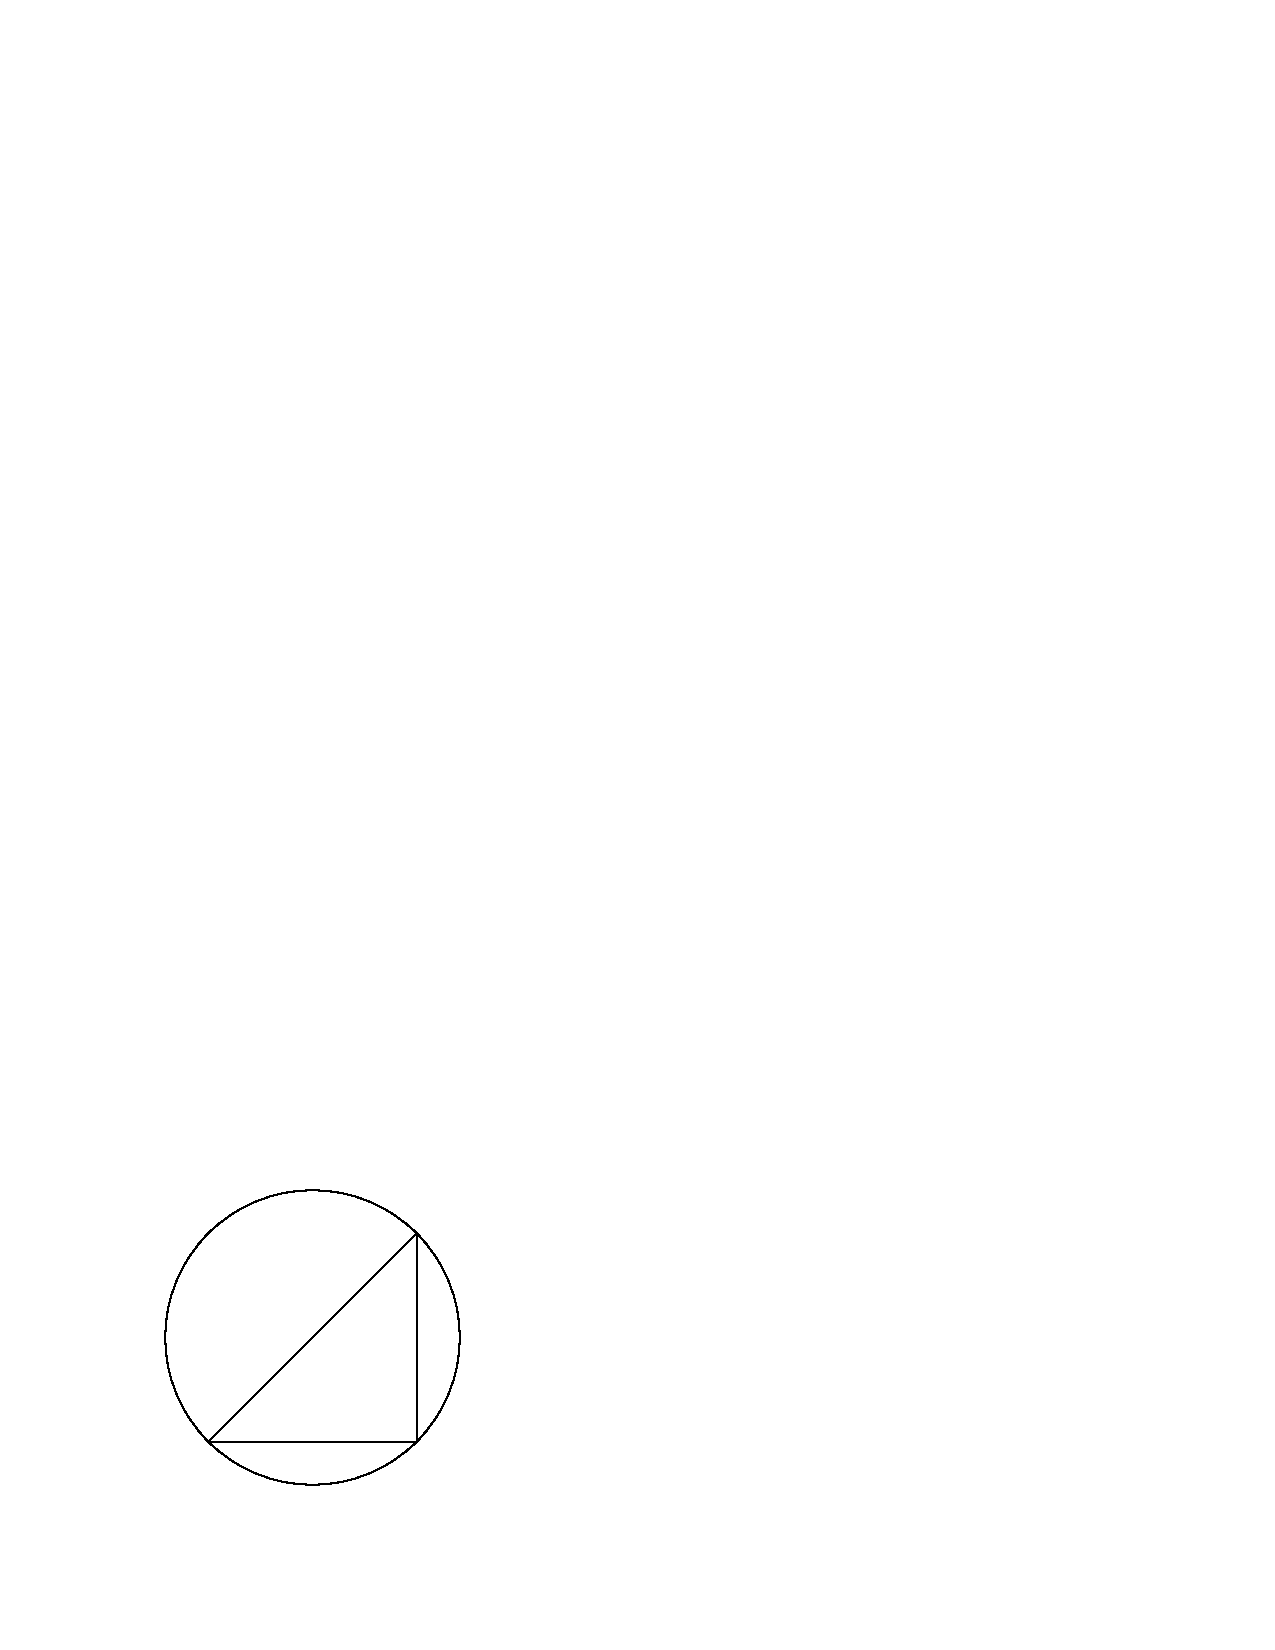
\includegraphics[clip,bb={74 74 225 225}]{images/mpsample}
  \caption{{\protect\MP}の出力例}\figlab{mpsample}
 \end{center}
\end{figure}
環境によっては日本語化された{\MP}を使うためには
\prog{mpost}ではなく\prog{jmpost}を使う事に
なるかもしれません.\Hito{角藤}{亮}の{\pTeX}を
使っているWindowsの方は\prog{jmpost}のはずです.


\subsection{\textsf{PSTricks}}
\Person{Timothy}{Zandt}らによる\Sty{PSTricks}は \cmd{special}命
令中に{\PS}命令を記述する事によって{\PS}の描画機能を
{\laTEX}で使えるようにするパッケージです.{\PS}命
令を多用する事からデバイスドライバとして\Prog{dvips}
などを想定していたり{\PS}対応プリンタでの使用が推奨され
ます.\sty{PSTricks}の詳しい使い方は日本語訳で70ページ分の
\wasyo{\GCOMP}\cite{graphicscomp}の第4章を参照してください.
基本的なマクロを読み込むためには\sty{PSTricks}パッケージを読み
込みます.特定のパッケージを個別に読み込む事もできます.
色を使うためには\sty{grahics}パッケージに含まれる\Sty{color}
パッケージではなく\Sty{pst-col}パッケージを読み込みます.全て
の機能を使うときは\Sty{pst-all}を読み込ます.標準的に以下のよ
うにするとうまく行くと思います.

\begin{InTeX}
\usepackage[dvips]{graphicx}
\usepackage[dvips,usenames]{pst-col} 
\usepackage{pst-all}
\end{InTeX}

具体的に\Z{三次元射影},画像のEPS変換,\Z{グラデーション},
\Z{木構造},\Z{回路図},\Z{プロット}などさまざまな事ができます.
%\kutiref{pstricks}に状態遷移図の例を示します.

\sty{PSTricks}を\Prog[dvipdfmx]{\Dvipdfmx}で
使うにはまず面倒な方法として\sty{PSTricks}を
使って描いた図形を一つ一つEPSファイルに変換する方法があります.

\begin{InTeX}
\documentclass{jsarticle}
\usepackage[dvips]{graphicx}
\usepackage[dvips,usenames]{pst-col} 
\usepackage{pst-all}
\pagestyle{empty}
\begin{document}
\begin{pspicture}(100,100)
 描画内容
\end{pspicture}
\end{document}
\end{InTeX}

このようなファイル\fl{fig1.tex}を作成し,これをコンソールから
次のようにします.
\begin{InTerm}
\type{platex fig1}
\type{dvipsk -Pdl -E -o fig1.eps fig1}
\type{epstopdf fig1.eps}
\type{egrep} \verb|"^%%BoundingBox:" fig1.eps > fig1.bb|
\end{InTerm}

上記の操作を図形の数だけこなし,図形を使用したい
{\LaTeX}の原稿にPDFファイル\fl{fig1.pdf}として
\sty{graphicx}の \cmd{includegraphics}で張り込みます.

\begin{InTeX}
\usepackage[dvipdfmx]{graphicx}
\includegrpahics[bb={0 0 100 100}]{fig1.pdf}
\end{InTeX}

\Person{CV}{Radhakrishnan}と\Person{CV}{Rajagopal}らに
よる\Sty{pdftricks}を使うと少しは楽になります.
これはもともと\prog{pdf\TeX}で\sty{PSTricks}を
使うためのものですが,\prog{\pLaTeX}にも流用でき
そうです.まずは\sty{pdftricks}に付属の
\Prog{pst2pdf}というシェルスクリプトを少し変更
します.

\begin{InText}
for f in $FIGURES ; do
  latex $fig
  dvips -Ppdf -E -o $fig.eps $fig
  epstopdf $fig.eps 
done
\end{InText}

この部分で\qu{\str{latex}}はもちろん\qu{\str{platex}}
にしますし.\qu{\str{dvips}}もご自分のシステムに
合うように変更してください.\Prog{epstopdf}で
変換したPDFのバウンディングボックスは正常ですが,
何かしらの問題があった時は次の1行も追加しておくと良いでしょう.

\begin{InText}
    egrep "^%%BoundingBox:"      $FILE > $fig.bb 
\end{InText}

%あとは
%\begin{InTerm}
%   \type{platex file}
%   \type{pst2pdf file}
%   \type{platex file}
%   \type{dvipdfmx file}
%\end{InTerm}
%のような作業をします.
%\sty{graphicx}と\sty{color}
%パッケージを読み込むときは
%\begin{InText}
%\usepackage[dvipdfm]{graphicx,color} 
%\end{InText}
%のように\Option{dvipdfm}を付けます.

\subsection{Xy-pic}
\Z{ダイアグラム}などを描くには\Person{Kristoffer}{Rose}と
\Person{Ross}{Moore}による\Prog[Xy-pic]{\Xy-pic}パッケ
ージを使うと良いでしょう.\Z{状態遷移図}や\Z{オートマトン},
\Z{回路図}などを描く事ができ非常に洗練されたシステムに
なっています.詳細は\wasyo{\GCOMP}\cite{graphicscomp}
の第5章を参照してください.

\subsection{化学式・化学構造式}\zindind{化学}{式}\zindind{化学}{構造式}
化学式や化学構造式を描くためには,\Hito{藤田}{眞作}による
\ruby{\XyMTeX}{きゅむてふ}パッケージを使うと良い
でしょう.これは{\LaTeX}の\env{picture}環境と
\sty{epic}を使ってベンゼン環やその他多くの化学式を
描く事ができます.\Prog[XyMTeX]{\XyMTeX}について
詳しく知りたい方は\hito{藤田}{眞作}の書いた
\yousyo{\XyMTeX}~\cite{xymtex}を参照してください.


%\subsection{チェスや将棋}
%レポートや論文で楽譜やチェス,将棋などの図を
%描く人は少数だと思いますが,詳しいことは
%\wasyo{\GCOMP}\cite{graphicscomp}の第7章と
%第8章を参照してください.
%
% hoge hoge


\subsection{グラフの描画}\seclab{gnuplot}
{\LaTeX}にグラフを挿入するには様々な方法が
あります.Windowsの方でならば{Excel}で作成した
グラフをEPSで保存し,それを\textsf{graphicx}パ
ッケージで読み込むという方法\pp{\secref{picture:program}参照}があります.
巷の表計算ソフトなんて使いたくない方は
\Person{Thomas}{Williams}と\Person{Colin}{Kelley}らによる
\Prog{Gnuplot}を使うと良いでしょう.\prog{gnuplot}
はバージョン3.7に関しては\Hito{山賀}{正人}が,バージョ
ン3.8に関しては\Hito{尾田}{晃}がプログラムの日本語化を
されています.また\prog{gnuplot}のマニュアルに
関しても\Hito{竹野}{茂治}らによって行われています\footnote{\webGplotman}.

\Z{制御系}では\Prog{SciLab}というのがあります.
マニュアルが\Hito{大野}{修一}らによって日本語化されています\footnote{\webScilabman}.

\Person{John}{Eaton}らによる\Prog{Octave}というのもあります
ので調べてみてください.

\endinput

%本書ではグラフ描画のためのプロットソフトの解説をしません.
%すでに沢山の参考書や日本語化マニュアルがありますので,
%\appref{info}を参照してください.

%
%
%\subsection{基本的な操作}
%まず{Gnuplot}は対話型のソフトウェアです.対話型とは描く図形などの
%オプションなどを指定しながら設定を確認していく形態のことです.
%{Windows}版の{Gnuplot}をインストールし,`\texttt{Readme}'を読んだ後,
%\texttt{wgnuplot}を実行すれば,
%\begin{quote}
%\verb+gnuplot> +
%\end{quote}
%という状態にあると思います.ユーザからの入力を待機している状態です.
%動きは{Unix}系のシェルに似ています.
%ワーキングディレクトリの概念もあります.
%終了は\texttt{exit}でも閉じるボタンでもかまいません.
%ここで
%\begin{quote}
%\verb+gnuplot> help+
%\end{quote}
%とすれば{Windows}ならば英語のヘルプが表示されるでしょう.
%例題つきでわかりやすいものですので,一度通して読んでみる
%ことをお勧めします.
%
%何かグラフを表示してみましょう.
%\begin{quote}
%\verb+gnuplot>plot sin(x)+
%\end{quote}
%とすれば別ウィンドウに正弦波sin関数が表示されたと思います.
%\subsection{覚えるコマンド}
%まずはこれだけは押さえておいたほうが良いコマンドを\tabref{gnuplotcmd}
%に記します.ルールとしてファイル名やディレクトリ名,ラベル名など,
%文字列はシングルクオートかダブルクオートで囲むことが必要です.
%\begin{table}[htbp]
%\caption{{Gnuplot}の基本コマンド}\tablab{gnuplotcmd}
%\begin{center}
%\begin{tabular}{|l|l|l|}
%\hline
%命令 & 説明 & 引数 \\
%\hline
%\texttt{exit}   & {Gnuplot}を終了します & なし \\
%\texttt{cd}     & 作業フォルダを変更します &  'ディレクトリ名'\\
%\texttt{pwd}    & 現在の作業フォルダを表示します & なし \\
%\texttt{help}   & ヘルプを表示します &  キーワード\\
%\texttt{load}   & ファイルを読み込みます &  'ファイル名'\\
%\texttt{plot}   & 2次元で関数やデータをプロットします & 関数など \\
%\texttt{splot}  & 3次元で関数やデータをプロットします & 関数など \\
%\texttt{multiplot}&複数の関数やデータを一つの窓に表示します& 関数など\\
%\texttt{replot} & 一度表示したものをもう一度プロットし直します & なし \\
%\texttt{set}    & オプションを設定します & 多種 \\
%\hline
%\end{tabular}
%\end{center}
%\end{table}
%ともかく,\texttt{plot}というコマンドで何でも描くということです.
%\texttt{plot}コマンドでは複数の関数,複数のデータ
%(\secref{gnuplotdatafile}参照)をプロットすることが可能です.
%また,変数や定数の定義は`A=35'などのように単純にできます.
%
%\subsection{関数と演算子}\seclab{gnuplot:functions}
%次に定義済みの関数についてです.
%Gnuplotでは様々な関数が用意されています.
%ほとんどの定義済み関数は`関数(変数$x$)',
%`sin($x$)'のように使います.
%\tabref{gnuplot:functions}に主要な定義済み関数を載せておきます.
%\begin{table}[htbp]
%\caption{Gnuplotの主な定義済み関数}
%\tablab{gnuplot:functions}
%\begin{center}
%\begin{tabular}{|ll|ll|}
%\hline
%関数     & 説明         &  関数    &  説明 \\
%\hline
%\verb+sin(x)+   & 正弦         & \verb+log(x)+   & 自然対数\\
%\verb+asin(x)+  & 逆正弦       & \verb+log10(x)+ & 常用対数\\
%\verb+asinh(x)+ & 逆双曲線正弦 & \verb+exp(x)+   & 指数関数\\
%\verb+cos(x)+   & 余弦         & \verb+int(x)+   & $x$の整数\\
%\verb+acos(x)+  & 逆余弦       & \verb+sqrt(x)+  & $x$の平方根\\
%\verb+asinh(x)+ & 逆双曲線余弦 & \verb+abs(x)+   & $x$の絶対値\\
%\verb+tan(x)+   & 正接         & \verb+rand(x)+  & 0から1未満の乱数$\times x$\\
%\verb+atan(x)+  & 逆正接       & \verb+imag(z)+  & zの虚部\\
%\verb+atanh(x)+ & 逆双曲線正接 & \verb+real(z)+  & zの実部\\
%\hline
%\end{tabular}
%\end{center}
%\end{table}
%以上のコマンドと関数を理解したら,
%今度はそれに関わる\Z{演算子}で値を
%操作します.演算子の表記方法はC言語と似ています.
%`似ている'というのは表現のうえだけではなく,処理のうえでもそうです.
%整数同士の除算の答え,例えば`$7/2=3$'となり,必ず整数になります.
%また,演算子によっては整数同士のみのものもあります.
%表現において,べき乗だけ表記方法が違って,
%FORTRANのようにアスタリスク`*'を二つ続けて`**'と表現します.
%演算子は単項演算子(Unary),二項演算子(Binary),
%三項演算子(Ternary)からなります.
%Gnuplotの主な演算子は\tabref{gnuplot:Operators}の通りです.
%なお,各演算子の優先順位はC言語とほぼ同じですので適宜
%括弧`()'で括るなどで対応してください.
%\begin{table}[htbp]
%\caption{Gnuplotの主な演算子}
%\tablab{gnuplot:Operators}
%\begin{center}
%*の付いている演算子の引数は整数に限ります\\
%\begin{tabular}{|l|l|l@{$= $ }l|}
%\hline
%演算子    & 説明             & 例   & 出力例 \\\hline
%\multicolumn{4}{|c|}{1項演算子}\\\hline
%\verb+-+ & 負                & -5   & -5     \\
%\verb-+- & 正                & +5   & +5     \\
%\verb+!+ & *階乗             & 4!   & 24     \\
%\verb+$+ & *`using'時の列指定& \$ 3 &        \\\hline
%\multicolumn{4}{|c|}{2項演算子}\\\hline
%\verb+**+& べき乗            & 2**10& 1024   \\
%\verb+*+ & 乗算              & 2*5  & 10     \\
%\verb+/+ & 除算              & 7/2  & 3      \\
%\verb+%+ & *剰余             & 7\%2 & 1      \\
%\verb-+- & 加算              & 7+2  & 9      \\
%\verb+-+ & 減算              & 7-2  & 5      \\\hline
%\end{tabular}
%\end{center}
%\end{table}
%
%\subsection{オプションの設定}
%しかし,これだけでは満足のいくグラフが描けません.通常$x$軸のラベルや
%範囲指定などが必要になります.そのようなときは`\texttt{set}'
%コマンドを使います.Gnuplotは\texttt{set}コマンドでグラ
%フに関する設定を行います.主なオプションを
%\tabref{gnuplot:options}に示します.
%
%\begin{table}[htbp]
%\caption{Gnuplotの主要オプション}\tablab{gnuplot:options}
%\begin{center}
%`()'の値は任意です.`\{\}'の値はいずれか一つを選びます.\\
%\begin{tabular}{|l|l|l|}
%\hline
%項目               & 説明 & 引数 \\\hline
%\verb+data style+         & データの表示形式の指定 & \texttt{lines,points,...}\\
%\verb+function style+     & 関数の表示形式の指定   & \texttt{lines,points,...}\\
%\verb+(no)grid+           & 格子線の(非)表示       & \texttt{(no)x(2)tics}\\
%\verb+(no)key+            & 名前の(非)表示         & \texttt{left,right,...}\\
%\verb+(no)logscale+       & 対数目盛に(しない)する & \texttt{x,y,z,xy,...}\\
%\verb+output+             & 出力先の指定           & \texttt{'filename.tex'} \\
%\verb+{xyz}(2)range+      & 各軸の範囲指定         & \verb+[最小値:最大値]+ \\
%\verb+samples+            & プロットする精度       & 1より大きい値\\
%\verb+size 幅,高さ+       & 出力するグラフの大きさ & $0<$値$\leq 1$\\
%\verb+terminal+           & 出力デバイスの設定     & \texttt{eepic,tgif,...}\\
%\verb+(no){xyz}(2)tics+   & 目盛りの付け方の指定   & 初期値,間隔,終値\\
%\verb+(no){xyz}(2)label+  & 各ラベルの指定         & '表示する名前'\\\hline
%\end{tabular}
%\end{center}
%\end{table}
%使い方は
%\begin{quote}
%\verb+gnuplot> set 項目 引数1 引数2...+\\
%\verb+gnuplot> set xtics 0,1,10+
%\end{quote}
%するだけです.
%
%\begin{comment}
%もう少しわかりやすく実際のグラフと対応させると\figref{gnuplot:taiou}
%となります.
%\begin{figure}[htbp]
%  \begin{center}
%  \begin{minipage}{.9\textwidth}
%    \begin{minipage}{.47\textwidth}
%      \begin{center}
%        \input{gnuplottaiou1}
%        (a)オプションの項目
%      \end{center}
%    \end{minipage}
%  \hfill
%    \begin{minipage}{.47\textwidth}
%      \begin{center}
%        \input{gnuplottaiou2}
%        (b)日本語での解説
%      \end{center}
%    \end{minipage}
%  \end{minipage}
%  \caption{Gnuplotオプションの図解}\figlab{gnuplot:taiou}
%  \end{center}
%\end{figure}
%\figref{gnuplot:taiou}(a)のほうがオプションの項目に対応し,
%\figref{gnuplot:taiou}(b)が日本語での説明です.
%\end{comment}
%
%\subsection{注意すべきこと}
%演算子の優先順位や,演算精度についてはおおよそC言語と同じなので,
%C言語を知っていればすぐに使いこなせると思います.
%しかし,整数値と軸については注意が必要です.
%まず整数値についてですが,Gnuplotは値が整数で与えられると,演算もその
%整数を優先します.とりあえず,与えるデータは小数のほうが結果の精度が
%良いようです.また,軸についてですが,Gnuplotでは軸の指定が二つあります.
%
%\subsection{データファイルからの読み込み}\seclab{gnuplotdatafile}
%シェルや\Prog{Cygwin}を開きましょう.\Prog{perl}で
%簡単なスクリプトを書きます.
% このスクリプトは結果的にGnuplot
%で$-10 \leqq  x \leqq 10$の範囲で$ y = x^3 $のグラフをプロットしてくれます.
%まず,以下のような`\texttt{Xcubed.pl}'を作成します.
%\begin{quote}
%\verb?for($i=-10.0; $i<=10; $i+=0.1){print "$i ",$i*$i*$i,"\n";}?
%\end{quote}
%というファイルを作ったとします.
%それで,
%\begin{InTerm}
%   \type{perl Xcubed.pl > plot.dat}
%\end{InTerm}
%として,この出力結果を`\texttt{plot.dat}'というファイルに
%書き出します.`\texttt{plot.dat}'の内容は以下の\figref{plot.dat}のようになります.
%\begin{figure}[htbp]
%\begin{center}
%\begin{InText}
%-10               -1000
%-9.9              -970.299
%...etc...
%9.89999999999996  970.298999999989
%9.99999999999996  999.999999999989
%\end{InText}
%\end{center}
%\caption{Perlで出力された`plot.dat'の内容}\figlab{plot.dat}
%\end{figure}
%このデータはn行2列のデータになっています.
%そうしたら,今度はGnuplotを起動して
%\begin{InTerm}
%gnuplot >  plot 'plot.dat'
%\end{InTerm}
%とすれば,$y=x^3$のグラフが描けます.
%その結果が\figref{gnuplot1}(a)`オプション指定なし'になります.
%\begin{figure}[htbp]
%    \begin{minipage}{.47\textwidth}
%      \begin{center}
%        % GNUPLOT: LaTeX picture using EEPIC macros
\setlength{\unitlength}{0.23pt}
\begin{picture}(750,450)(0,0)
\footnotesize
\thicklines \path(176,90)(196,90)
\thicklines \path(683,90)(663,90)
\put(154,90){\makebox(0,0)[r]{-1000}}
\thicklines \path(176,122)(196,122)
\thicklines \path(683,122)(663,122)
\put(154,122){\makebox(0,0)[r]{-800}}
\thicklines \path(176,153)(196,153)
\thicklines \path(683,153)(663,153)
\put(154,153){\makebox(0,0)[r]{-600}}
\thicklines \path(176,185)(196,185)
\thicklines \path(683,185)(663,185)
\put(154,185){\makebox(0,0)[r]{-400}}
\thicklines \path(176,216)(196,216)
\thicklines \path(683,216)(663,216)
\put(154,216){\makebox(0,0)[r]{-200}}
\thicklines \path(176,248)(196,248)
\thicklines \path(683,248)(663,248)
\put(154,248){\makebox(0,0)[r]{0}}
\thicklines \path(176,280)(196,280)
\thicklines \path(683,280)(663,280)
\put(154,280){\makebox(0,0)[r]{200}}
\thicklines \path(176,311)(196,311)
\thicklines \path(683,311)(663,311)
\put(154,311){\makebox(0,0)[r]{400}}
\thicklines \path(176,343)(196,343)
\thicklines \path(683,343)(663,343)
\put(154,343){\makebox(0,0)[r]{600}}
\thicklines \path(176,374)(196,374)
\thicklines \path(683,374)(663,374)
\put(154,374){\makebox(0,0)[r]{800}}
\thicklines \path(176,406)(196,406)
\thicklines \path(683,406)(663,406)
\put(154,406){\makebox(0,0)[r]{1000}}
\thicklines \path(176,90)(176,110)
\thicklines \path(176,406)(176,386)
\put(176,45){\makebox(0,0){-10}}
\thicklines \path(227,90)(227,110)
\thicklines \path(227,406)(227,386)
\put(227,45){\makebox(0,0){-8}}
\thicklines \path(277,90)(277,110)
\thicklines \path(277,406)(277,386)
\put(277,45){\makebox(0,0){-6}}
\thicklines \path(328,90)(328,110)
\thicklines \path(328,406)(328,386)
\put(328,45){\makebox(0,0){-4}}
\thicklines \path(379,90)(379,110)
\thicklines \path(379,406)(379,386)
\put(379,45){\makebox(0,0){-2}}
\thicklines \path(430,90)(430,110)
\thicklines \path(430,406)(430,386)
\put(430,45){\makebox(0,0){0}}
\thicklines \path(480,90)(480,110)
\thicklines \path(480,406)(480,386)
\put(480,45){\makebox(0,0){2}}
\thicklines \path(531,90)(531,110)
\thicklines \path(531,406)(531,386)
\put(531,45){\makebox(0,0){4}}
\thicklines \path(582,90)(582,110)
\thicklines \path(582,406)(582,386)
\put(582,45){\makebox(0,0){6}}
\thicklines \path(632,90)(632,110)
\thicklines \path(632,406)(632,386)
\put(632,45){\makebox(0,0){8}}
\thicklines \path(683,90)(683,110)
\thicklines \path(683,406)(683,386)
\put(683,45){\makebox(0,0){10}}
\thicklines \path(176,90)(683,90)(683,406)(176,406)(176,90)
\put(509,364){\makebox(0,0)[r]{"plot.dat"}}
\put(176,90){\raisebox{-1.2pt}{\makebox(0,0){$\Diamond$}}}
\put(179,95){\raisebox{-1.2pt}{\makebox(0,0){$\Diamond$}}}
\put(181,99){\raisebox{-1.2pt}{\makebox(0,0){$\Diamond$}}}
\put(184,104){\raisebox{-1.2pt}{\makebox(0,0){$\Diamond$}}}
\put(186,108){\raisebox{-1.2pt}{\makebox(0,0){$\Diamond$}}}
\put(189,113){\raisebox{-1.2pt}{\makebox(0,0){$\Diamond$}}}
\put(191,117){\raisebox{-1.2pt}{\makebox(0,0){$\Diamond$}}}
\put(194,121){\raisebox{-1.2pt}{\makebox(0,0){$\Diamond$}}}
\put(196,125){\raisebox{-1.2pt}{\makebox(0,0){$\Diamond$}}}
\put(199,129){\raisebox{-1.2pt}{\makebox(0,0){$\Diamond$}}}
\put(201,133){\raisebox{-1.2pt}{\makebox(0,0){$\Diamond$}}}
\put(204,137){\raisebox{-1.2pt}{\makebox(0,0){$\Diamond$}}}
\put(206,140){\raisebox{-1.2pt}{\makebox(0,0){$\Diamond$}}}
\put(209,144){\raisebox{-1.2pt}{\makebox(0,0){$\Diamond$}}}
\put(211,148){\raisebox{-1.2pt}{\makebox(0,0){$\Diamond$}}}
\put(214,151){\raisebox{-1.2pt}{\makebox(0,0){$\Diamond$}}}
\put(217,154){\raisebox{-1.2pt}{\makebox(0,0){$\Diamond$}}}
\put(219,158){\raisebox{-1.2pt}{\makebox(0,0){$\Diamond$}}}
\put(222,161){\raisebox{-1.2pt}{\makebox(0,0){$\Diamond$}}}
\put(224,164){\raisebox{-1.2pt}{\makebox(0,0){$\Diamond$}}}
\put(227,167){\raisebox{-1.2pt}{\makebox(0,0){$\Diamond$}}}
\put(229,170){\raisebox{-1.2pt}{\makebox(0,0){$\Diamond$}}}
\put(232,173){\raisebox{-1.2pt}{\makebox(0,0){$\Diamond$}}}
\put(234,176){\raisebox{-1.2pt}{\makebox(0,0){$\Diamond$}}}
\put(237,179){\raisebox{-1.2pt}{\makebox(0,0){$\Diamond$}}}
\put(239,181){\raisebox{-1.2pt}{\makebox(0,0){$\Diamond$}}}
\put(242,184){\raisebox{-1.2pt}{\makebox(0,0){$\Diamond$}}}
\put(244,187){\raisebox{-1.2pt}{\makebox(0,0){$\Diamond$}}}
\put(247,189){\raisebox{-1.2pt}{\makebox(0,0){$\Diamond$}}}
\put(250,191){\raisebox{-1.2pt}{\makebox(0,0){$\Diamond$}}}
\put(252,194){\raisebox{-1.2pt}{\makebox(0,0){$\Diamond$}}}
\put(255,196){\raisebox{-1.2pt}{\makebox(0,0){$\Diamond$}}}
\put(257,198){\raisebox{-1.2pt}{\makebox(0,0){$\Diamond$}}}
\put(260,200){\raisebox{-1.2pt}{\makebox(0,0){$\Diamond$}}}
\put(262,203){\raisebox{-1.2pt}{\makebox(0,0){$\Diamond$}}}
\put(265,205){\raisebox{-1.2pt}{\makebox(0,0){$\Diamond$}}}
\put(267,207){\raisebox{-1.2pt}{\makebox(0,0){$\Diamond$}}}
\put(270,208){\raisebox{-1.2pt}{\makebox(0,0){$\Diamond$}}}
\put(272,210){\raisebox{-1.2pt}{\makebox(0,0){$\Diamond$}}}
\put(275,212){\raisebox{-1.2pt}{\makebox(0,0){$\Diamond$}}}
\put(277,214){\raisebox{-1.2pt}{\makebox(0,0){$\Diamond$}}}
\put(280,216){\raisebox{-1.2pt}{\makebox(0,0){$\Diamond$}}}
\put(282,217){\raisebox{-1.2pt}{\makebox(0,0){$\Diamond$}}}
\put(285,219){\raisebox{-1.2pt}{\makebox(0,0){$\Diamond$}}}
\put(288,220){\raisebox{-1.2pt}{\makebox(0,0){$\Diamond$}}}
\put(290,222){\raisebox{-1.2pt}{\makebox(0,0){$\Diamond$}}}
\put(293,223){\raisebox{-1.2pt}{\makebox(0,0){$\Diamond$}}}
\put(295,224){\raisebox{-1.2pt}{\makebox(0,0){$\Diamond$}}}
\put(298,226){\raisebox{-1.2pt}{\makebox(0,0){$\Diamond$}}}
\put(300,227){\raisebox{-1.2pt}{\makebox(0,0){$\Diamond$}}}
\put(303,228){\raisebox{-1.2pt}{\makebox(0,0){$\Diamond$}}}
\put(305,229){\raisebox{-1.2pt}{\makebox(0,0){$\Diamond$}}}
\put(308,231){\raisebox{-1.2pt}{\makebox(0,0){$\Diamond$}}}
\put(310,232){\raisebox{-1.2pt}{\makebox(0,0){$\Diamond$}}}
\put(313,233){\raisebox{-1.2pt}{\makebox(0,0){$\Diamond$}}}
\put(315,234){\raisebox{-1.2pt}{\makebox(0,0){$\Diamond$}}}
\put(318,235){\raisebox{-1.2pt}{\makebox(0,0){$\Diamond$}}}
\put(320,235){\raisebox{-1.2pt}{\makebox(0,0){$\Diamond$}}}
\put(323,236){\raisebox{-1.2pt}{\makebox(0,0){$\Diamond$}}}
\put(326,237){\raisebox{-1.2pt}{\makebox(0,0){$\Diamond$}}}
\put(328,238){\raisebox{-1.2pt}{\makebox(0,0){$\Diamond$}}}
\put(331,239){\raisebox{-1.2pt}{\makebox(0,0){$\Diamond$}}}
\put(333,239){\raisebox{-1.2pt}{\makebox(0,0){$\Diamond$}}}
\put(336,240){\raisebox{-1.2pt}{\makebox(0,0){$\Diamond$}}}
\put(338,241){\raisebox{-1.2pt}{\makebox(0,0){$\Diamond$}}}
\put(341,241){\raisebox{-1.2pt}{\makebox(0,0){$\Diamond$}}}
\put(343,242){\raisebox{-1.2pt}{\makebox(0,0){$\Diamond$}}}
\put(346,242){\raisebox{-1.2pt}{\makebox(0,0){$\Diamond$}}}
\put(348,243){\raisebox{-1.2pt}{\makebox(0,0){$\Diamond$}}}
\put(351,243){\raisebox{-1.2pt}{\makebox(0,0){$\Diamond$}}}
\put(353,244){\raisebox{-1.2pt}{\makebox(0,0){$\Diamond$}}}
\put(356,244){\raisebox{-1.2pt}{\makebox(0,0){$\Diamond$}}}
\put(359,245){\raisebox{-1.2pt}{\makebox(0,0){$\Diamond$}}}
\put(361,245){\raisebox{-1.2pt}{\makebox(0,0){$\Diamond$}}}
\put(364,245){\raisebox{-1.2pt}{\makebox(0,0){$\Diamond$}}}
\put(366,246){\raisebox{-1.2pt}{\makebox(0,0){$\Diamond$}}}
\put(369,246){\raisebox{-1.2pt}{\makebox(0,0){$\Diamond$}}}
\put(371,246){\raisebox{-1.2pt}{\makebox(0,0){$\Diamond$}}}
\put(374,246){\raisebox{-1.2pt}{\makebox(0,0){$\Diamond$}}}
\put(376,247){\raisebox{-1.2pt}{\makebox(0,0){$\Diamond$}}}
\put(379,247){\raisebox{-1.2pt}{\makebox(0,0){$\Diamond$}}}
\put(381,247){\raisebox{-1.2pt}{\makebox(0,0){$\Diamond$}}}
\put(384,247){\raisebox{-1.2pt}{\makebox(0,0){$\Diamond$}}}
\put(386,247){\raisebox{-1.2pt}{\makebox(0,0){$\Diamond$}}}
\put(389,247){\raisebox{-1.2pt}{\makebox(0,0){$\Diamond$}}}
\put(391,247){\raisebox{-1.2pt}{\makebox(0,0){$\Diamond$}}}
\put(394,248){\raisebox{-1.2pt}{\makebox(0,0){$\Diamond$}}}
\put(397,248){\raisebox{-1.2pt}{\makebox(0,0){$\Diamond$}}}
\put(399,248){\raisebox{-1.2pt}{\makebox(0,0){$\Diamond$}}}
\put(402,248){\raisebox{-1.2pt}{\makebox(0,0){$\Diamond$}}}
\put(404,248){\raisebox{-1.2pt}{\makebox(0,0){$\Diamond$}}}
\put(407,248){\raisebox{-1.2pt}{\makebox(0,0){$\Diamond$}}}
\put(409,248){\raisebox{-1.2pt}{\makebox(0,0){$\Diamond$}}}
\put(412,248){\raisebox{-1.2pt}{\makebox(0,0){$\Diamond$}}}
\put(414,248){\raisebox{-1.2pt}{\makebox(0,0){$\Diamond$}}}
\put(417,248){\raisebox{-1.2pt}{\makebox(0,0){$\Diamond$}}}
\put(419,248){\raisebox{-1.2pt}{\makebox(0,0){$\Diamond$}}}
\put(422,248){\raisebox{-1.2pt}{\makebox(0,0){$\Diamond$}}}
\put(424,248){\raisebox{-1.2pt}{\makebox(0,0){$\Diamond$}}}
\put(427,248){\raisebox{-1.2pt}{\makebox(0,0){$\Diamond$}}}
\put(429,248){\raisebox{-1.2pt}{\makebox(0,0){$\Diamond$}}}
\put(432,248){\raisebox{-1.2pt}{\makebox(0,0){$\Diamond$}}}
\put(435,248){\raisebox{-1.2pt}{\makebox(0,0){$\Diamond$}}}
\put(437,248){\raisebox{-1.2pt}{\makebox(0,0){$\Diamond$}}}
\put(440,248){\raisebox{-1.2pt}{\makebox(0,0){$\Diamond$}}}
\put(442,248){\raisebox{-1.2pt}{\makebox(0,0){$\Diamond$}}}
\put(445,248){\raisebox{-1.2pt}{\makebox(0,0){$\Diamond$}}}
\put(447,248){\raisebox{-1.2pt}{\makebox(0,0){$\Diamond$}}}
\put(450,248){\raisebox{-1.2pt}{\makebox(0,0){$\Diamond$}}}
\put(452,248){\raisebox{-1.2pt}{\makebox(0,0){$\Diamond$}}}
\put(455,248){\raisebox{-1.2pt}{\makebox(0,0){$\Diamond$}}}
\put(457,248){\raisebox{-1.2pt}{\makebox(0,0){$\Diamond$}}}
\put(460,248){\raisebox{-1.2pt}{\makebox(0,0){$\Diamond$}}}
\put(462,248){\raisebox{-1.2pt}{\makebox(0,0){$\Diamond$}}}
\put(465,248){\raisebox{-1.2pt}{\makebox(0,0){$\Diamond$}}}
\put(468,249){\raisebox{-1.2pt}{\makebox(0,0){$\Diamond$}}}
\put(470,249){\raisebox{-1.2pt}{\makebox(0,0){$\Diamond$}}}
\put(473,249){\raisebox{-1.2pt}{\makebox(0,0){$\Diamond$}}}
\put(475,249){\raisebox{-1.2pt}{\makebox(0,0){$\Diamond$}}}
\put(478,249){\raisebox{-1.2pt}{\makebox(0,0){$\Diamond$}}}
\put(480,249){\raisebox{-1.2pt}{\makebox(0,0){$\Diamond$}}}
\put(483,249){\raisebox{-1.2pt}{\makebox(0,0){$\Diamond$}}}
\put(485,250){\raisebox{-1.2pt}{\makebox(0,0){$\Diamond$}}}
\put(488,250){\raisebox{-1.2pt}{\makebox(0,0){$\Diamond$}}}
\put(490,250){\raisebox{-1.2pt}{\makebox(0,0){$\Diamond$}}}
\put(493,250){\raisebox{-1.2pt}{\makebox(0,0){$\Diamond$}}}
\put(495,251){\raisebox{-1.2pt}{\makebox(0,0){$\Diamond$}}}
\put(498,251){\raisebox{-1.2pt}{\makebox(0,0){$\Diamond$}}}
\put(500,251){\raisebox{-1.2pt}{\makebox(0,0){$\Diamond$}}}
\put(503,252){\raisebox{-1.2pt}{\makebox(0,0){$\Diamond$}}}
\put(506,252){\raisebox{-1.2pt}{\makebox(0,0){$\Diamond$}}}
\put(508,253){\raisebox{-1.2pt}{\makebox(0,0){$\Diamond$}}}
\put(511,253){\raisebox{-1.2pt}{\makebox(0,0){$\Diamond$}}}
\put(513,254){\raisebox{-1.2pt}{\makebox(0,0){$\Diamond$}}}
\put(516,254){\raisebox{-1.2pt}{\makebox(0,0){$\Diamond$}}}
\put(518,255){\raisebox{-1.2pt}{\makebox(0,0){$\Diamond$}}}
\put(521,255){\raisebox{-1.2pt}{\makebox(0,0){$\Diamond$}}}
\put(523,256){\raisebox{-1.2pt}{\makebox(0,0){$\Diamond$}}}
\put(526,257){\raisebox{-1.2pt}{\makebox(0,0){$\Diamond$}}}
\put(528,257){\raisebox{-1.2pt}{\makebox(0,0){$\Diamond$}}}
\put(531,258){\raisebox{-1.2pt}{\makebox(0,0){$\Diamond$}}}
\put(533,259){\raisebox{-1.2pt}{\makebox(0,0){$\Diamond$}}}
\put(536,260){\raisebox{-1.2pt}{\makebox(0,0){$\Diamond$}}}
\put(539,261){\raisebox{-1.2pt}{\makebox(0,0){$\Diamond$}}}
\put(541,261){\raisebox{-1.2pt}{\makebox(0,0){$\Diamond$}}}
\put(544,262){\raisebox{-1.2pt}{\makebox(0,0){$\Diamond$}}}
\put(546,263){\raisebox{-1.2pt}{\makebox(0,0){$\Diamond$}}}
\put(549,264){\raisebox{-1.2pt}{\makebox(0,0){$\Diamond$}}}
\put(551,265){\raisebox{-1.2pt}{\makebox(0,0){$\Diamond$}}}
\put(554,267){\raisebox{-1.2pt}{\makebox(0,0){$\Diamond$}}}
\put(556,268){\raisebox{-1.2pt}{\makebox(0,0){$\Diamond$}}}
\put(559,269){\raisebox{-1.2pt}{\makebox(0,0){$\Diamond$}}}
\put(561,270){\raisebox{-1.2pt}{\makebox(0,0){$\Diamond$}}}
\put(564,272){\raisebox{-1.2pt}{\makebox(0,0){$\Diamond$}}}
\put(566,273){\raisebox{-1.2pt}{\makebox(0,0){$\Diamond$}}}
\put(569,274){\raisebox{-1.2pt}{\makebox(0,0){$\Diamond$}}}
\put(571,276){\raisebox{-1.2pt}{\makebox(0,0){$\Diamond$}}}
\put(574,277){\raisebox{-1.2pt}{\makebox(0,0){$\Diamond$}}}
\put(577,279){\raisebox{-1.2pt}{\makebox(0,0){$\Diamond$}}}
\put(579,280){\raisebox{-1.2pt}{\makebox(0,0){$\Diamond$}}}
\put(582,282){\raisebox{-1.2pt}{\makebox(0,0){$\Diamond$}}}
\put(584,284){\raisebox{-1.2pt}{\makebox(0,0){$\Diamond$}}}
\put(587,286){\raisebox{-1.2pt}{\makebox(0,0){$\Diamond$}}}
\put(589,288){\raisebox{-1.2pt}{\makebox(0,0){$\Diamond$}}}
\put(592,289){\raisebox{-1.2pt}{\makebox(0,0){$\Diamond$}}}
\put(594,291){\raisebox{-1.2pt}{\makebox(0,0){$\Diamond$}}}
\put(597,293){\raisebox{-1.2pt}{\makebox(0,0){$\Diamond$}}}
\put(599,296){\raisebox{-1.2pt}{\makebox(0,0){$\Diamond$}}}
\put(602,298){\raisebox{-1.2pt}{\makebox(0,0){$\Diamond$}}}
\put(604,300){\raisebox{-1.2pt}{\makebox(0,0){$\Diamond$}}}
\put(607,302){\raisebox{-1.2pt}{\makebox(0,0){$\Diamond$}}}
\put(609,305){\raisebox{-1.2pt}{\makebox(0,0){$\Diamond$}}}
\put(612,307){\raisebox{-1.2pt}{\makebox(0,0){$\Diamond$}}}
\put(615,309){\raisebox{-1.2pt}{\makebox(0,0){$\Diamond$}}}
\put(617,312){\raisebox{-1.2pt}{\makebox(0,0){$\Diamond$}}}
\put(620,315){\raisebox{-1.2pt}{\makebox(0,0){$\Diamond$}}}
\put(622,317){\raisebox{-1.2pt}{\makebox(0,0){$\Diamond$}}}
\put(625,320){\raisebox{-1.2pt}{\makebox(0,0){$\Diamond$}}}
\put(627,323){\raisebox{-1.2pt}{\makebox(0,0){$\Diamond$}}}
\put(630,326){\raisebox{-1.2pt}{\makebox(0,0){$\Diamond$}}}
\put(632,329){\raisebox{-1.2pt}{\makebox(0,0){$\Diamond$}}}
\put(635,332){\raisebox{-1.2pt}{\makebox(0,0){$\Diamond$}}}
\put(637,335){\raisebox{-1.2pt}{\makebox(0,0){$\Diamond$}}}
\put(640,338){\raisebox{-1.2pt}{\makebox(0,0){$\Diamond$}}}
\put(642,342){\raisebox{-1.2pt}{\makebox(0,0){$\Diamond$}}}
\put(645,345){\raisebox{-1.2pt}{\makebox(0,0){$\Diamond$}}}
\put(648,348){\raisebox{-1.2pt}{\makebox(0,0){$\Diamond$}}}
\put(650,352){\raisebox{-1.2pt}{\makebox(0,0){$\Diamond$}}}
\put(653,356){\raisebox{-1.2pt}{\makebox(0,0){$\Diamond$}}}
\put(655,359){\raisebox{-1.2pt}{\makebox(0,0){$\Diamond$}}}
\put(658,363){\raisebox{-1.2pt}{\makebox(0,0){$\Diamond$}}}
\put(660,367){\raisebox{-1.2pt}{\makebox(0,0){$\Diamond$}}}
\put(663,371){\raisebox{-1.2pt}{\makebox(0,0){$\Diamond$}}}
\put(665,375){\raisebox{-1.2pt}{\makebox(0,0){$\Diamond$}}}
\put(668,379){\raisebox{-1.2pt}{\makebox(0,0){$\Diamond$}}}
\put(670,383){\raisebox{-1.2pt}{\makebox(0,0){$\Diamond$}}}
\put(673,388){\raisebox{-1.2pt}{\makebox(0,0){$\Diamond$}}}
\put(675,392){\raisebox{-1.2pt}{\makebox(0,0){$\Diamond$}}}
\put(678,397){\raisebox{-1.2pt}{\makebox(0,0){$\Diamond$}}}
\put(680,401){\raisebox{-1.2pt}{\makebox(0,0){$\Diamond$}}}
\put(683,406){\raisebox{-1.2pt}{\makebox(0,0){$\Diamond$}}}
\put(585,364){\raisebox{-1.2pt}{\makebox(0,0){$\Diamond$}}}
\end{picture}

%        \\(a)オプション指定なし
%      \end{center}
%    \end{minipage}
%  \hfill
%    \begin{minipage}{.47\textwidth}
%      \begin{center}
%        % GNUPLOT: LaTeX picture using EEPIC macros
\setlength{\unitlength}{0.23pt}
\begin{picture}(750,450)(0,0)
\footnotesize
\thinlines \drawline[-50](221,135)(683,135)
\thicklines \path(221,135)(241,135)
\thicklines \path(683,135)(663,135)
\put(199,135){\makebox(0,0)[r]{-1000}}
\thinlines \drawline[-50](221,203)(683,203)
\thicklines \path(221,203)(241,203)
\thicklines \path(683,203)(663,203)
\put(199,203){\makebox(0,0)[r]{-500}}
\thinlines \drawline[-50](221,271)(683,271)
\thicklines \path(221,271)(241,271)
\thicklines \path(683,271)(663,271)
\put(199,271){\makebox(0,0)[r]{0}}
\thinlines \drawline[-50](221,338)(683,338)
\thicklines \path(221,338)(241,338)
\thicklines \path(683,338)(663,338)
\put(199,338){\makebox(0,0)[r]{500}}
\thinlines \drawline[-50](221,406)(683,406)
\thicklines \path(221,406)(241,406)
\thicklines \path(683,406)(663,406)
\put(199,406){\makebox(0,0)[r]{1000}}
\thinlines \drawline[-50](221,135)(221,406)
\thicklines \path(221,135)(221,155)
\thicklines \path(221,406)(221,386)
\put(221,90){\makebox(0,0){-10}}
\thinlines \drawline[-50](337,135)(337,406)
\thicklines \path(337,135)(337,155)
\thicklines \path(337,406)(337,386)
\put(337,90){\makebox(0,0){-5}}
\thinlines \drawline[-50](452,135)(452,341)
\thinlines \drawline[-50](452,386)(452,406)
\thicklines \path(452,135)(452,155)
\thicklines \path(452,406)(452,386)
\put(452,90){\makebox(0,0){0}}
\thinlines \drawline[-50](568,135)(568,341)
\thinlines \drawline[-50](568,386)(568,406)
\thicklines \path(568,135)(568,155)
\thicklines \path(568,406)(568,386)
\put(568,90){\makebox(0,0){5}}
\thinlines \drawline[-50](683,135)(683,406)
\thicklines \path(683,135)(683,155)
\thicklines \path(683,406)(683,386)
\put(683,90){\makebox(0,0){10}}
\thicklines \path(221,135)(683,135)(683,406)(221,406)(221,135)
\put(44,270){\makebox(0,0)[l]{\shortstack{\rotatebox{90}{$y$}}}}
\put(452,23){\makebox(0,0){$x$}}
\put(509,364){\makebox(0,0)[r]{$x^3$}}
\thinlines \path(531,364)(639,364)
\thinlines \path(221,135)(221,135)(245,173)(270,204)(294,227)(318,244)(343,256)(367,264)(391,268)(416,270)(440,270)(464,271)(488,271)(513,273)(537,277)(561,285)(586,297)(610,314)(634,337)(659,368)(683,406)
\put(221,135){\raisebox{-1.2pt}{\makebox(0,0){$\Diamond$}}}
\put(245,173){\raisebox{-1.2pt}{\makebox(0,0){$\Diamond$}}}
\put(270,204){\raisebox{-1.2pt}{\makebox(0,0){$\Diamond$}}}
\put(294,227){\raisebox{-1.2pt}{\makebox(0,0){$\Diamond$}}}
\put(318,244){\raisebox{-1.2pt}{\makebox(0,0){$\Diamond$}}}
\put(343,256){\raisebox{-1.2pt}{\makebox(0,0){$\Diamond$}}}
\put(367,264){\raisebox{-1.2pt}{\makebox(0,0){$\Diamond$}}}
\put(391,268){\raisebox{-1.2pt}{\makebox(0,0){$\Diamond$}}}
\put(416,270){\raisebox{-1.2pt}{\makebox(0,0){$\Diamond$}}}
\put(440,270){\raisebox{-1.2pt}{\makebox(0,0){$\Diamond$}}}
\put(464,271){\raisebox{-1.2pt}{\makebox(0,0){$\Diamond$}}}
\put(488,271){\raisebox{-1.2pt}{\makebox(0,0){$\Diamond$}}}
\put(513,273){\raisebox{-1.2pt}{\makebox(0,0){$\Diamond$}}}
\put(537,277){\raisebox{-1.2pt}{\makebox(0,0){$\Diamond$}}}
\put(561,285){\raisebox{-1.2pt}{\makebox(0,0){$\Diamond$}}}
\put(586,297){\raisebox{-1.2pt}{\makebox(0,0){$\Diamond$}}}
\put(610,314){\raisebox{-1.2pt}{\makebox(0,0){$\Diamond$}}}
\put(634,337){\raisebox{-1.2pt}{\makebox(0,0){$\Diamond$}}}
\put(659,368){\raisebox{-1.2pt}{\makebox(0,0){$\Diamond$}}}
\put(683,406){\raisebox{-1.2pt}{\makebox(0,0){$\Diamond$}}}
\put(585,364){\raisebox{-1.2pt}{\makebox(0,0){$\Diamond$}}}
\end{picture}

%        \\(b)オプション指定あり
%      \end{center}
%    \end{minipage}
%  \caption{データからGnuplotへの読み込み}\figlab{gnuplot1}
%\end{figure}
%しかし,このままではまだ完全ではないと思います.オプションを幾つか指定して
%必要なものを追加しましょう.
%\figref{gnuplot1}(b)`オプション指定あり'は以下のGnuplotのコマンド
%で描画されています.
%\begin{quote}
%\begin{InText}
%cd 'D:\Gnuplot'
%set xlabel 'x' ;  set ylabel 'y'
%set data style linespoints
%set grid
%plot 'plot.dat'
%\end{InText}
%\end{quote}
%%$
%\subsection{GnuplotとExcelの連携}
%データファイルからの読み込みが可能になりました.
%これを応用してMicrosoftのExcelのデータも活用す
%ることができます.Excelには数多くの
%関数が用意されているので,大変便利です.
%そこで\tabref{excel2gnuplot}
%があったとします.
%\begin{table}[htbp]
%\caption{ExcelとGnuplotの連携}\label{excel2gnuplot}
%\begin{center}
%\begin{tabular}{|r|r|r|r|} \hline
%-5 & 0.11920  & 0.04743  & 0.00669  \\\hline
%-4 & 0.16798  & 0.08317  & 0.01799  \\\hline
%-3 & 0.23148  & 0.14185  & 0.04743  \\\hline
%-2 & 0.31003  & 0.23148  & 0.11920  \\\hline
%-1 & 0.40131  & 0.35434  & 0.26894  \\\hline
%0 & 0.50000  & 0.50000  & 0.50000  \\\hline
%1 & 0.59869  & 0.64566  & 0.73106  \\\hline
%2 & 0.68997  & 0.76852  & 0.88080  \\\hline
%3 & 0.76852  & 0.85815  & 0.95257  \\\hline
%4 & 0.83202  & 0.91683  & 0.98201  \\\hline
%5 & 0.88080  & 0.95257  & 0.99331  \\\hline
%\end{tabular}
%\end{center}
%\end{table}
%\tabref{excel2gnuplot}の内容をGnuplotで
%表示するには`\texttt{using}'コマンドを使います.
%まず,このデータをGnuplotでも使えるようなデータにするために,
%{Excel}のツールバーから\win{ファイル}を選び,
%\win{名前をつけて保存}でファイル形式を
%`テキスト(タブ区切り)'でファイル名を`excel.txt'と仮に保存します.
%このデータは11行4列のデータになっています.
%これを\texttt{plot}プロットコマンドで
%\begin{InTerm}
%gnuplot$>$ plot 'excel.txt'
%\end{InTerm}
%とすると,1列目が$x$軸,2列目が$y$軸の値としてプロットされます.
%これを自由自在に1列目と3列目,2列目と4列目などのように扱うには
%\begin{quote}
%\texttt{plot "ファイル名" using xの列:yの列}
%\end{quote}
%のように,プロットする関数に付け足します.
%先ほどの表から例(\figref{gnuplot:using})を示します.
%\begin{figure}[htbp]
%\begin{center}
%\begin{InText}
%> cd 'D:\MyThesis'
%> plot 'excel.txt' using 1:3,'excel.txt'
%      using 1:4 ,1/(1+exp(-x)) 
%\end{InText}
%\end{center}
%\caption{Gnuplotで`\texttt{using}'を使う例}\figlab{gnuplot:using}
%\end{figure}
%\begin{comment}
%\subsection{実験結果と理論値の一致}
%Gnuplotの機能の一つに,実験して得られた\tabref{excel2gnuplot}の
%ようなデータと方程式\equref{roji1})
%\begin{equation}\equlab{roji1}
%f(x) = \frac{A}{B+Ce^{-Dx}}
%\end{equation}
%を解析し,自動的に変数$A,B,C,D$を推定してくれます.
%3次元はもちろんのこと,非線形方程式も推定するので便利です.
%使い方は
%\begin{quote}
%\verb+fit 関数f(x) "データファイル名" via 変数のリスト+
%\end{quote}
%とします.まずは例の\figref{roji2}`\texttt{Fit.plt}'を見てください.
%\begin{figure}[htbp]\begin{center}
%\begin{InText}
%> f(x) = A/(B+C*exp(-D*x))
%> A=1 ; B=1 ; C=0.6 ; D= 0.6 ;
%> fit f(x) 'excel.txt' using 1:2 via A,B,C,D
%> plot f(x),'excel.txt' using 1:2,
%   1/(1+0.6*exp(-0.6*x))
%\end{InText}
%\caption{Gnuplotの`\texttt{fit}'の使用例}\figlab{roji2}
%\end{center}\end{figure}
%これにより,変数$A,B,C,D$の値が具体的に決まります.
%この解析結果は処理後に自動的に`\texttt{fit.log}'という
%ファイルに保存され,標準誤差などのデータを確認することができます.
%\end{comment}
%
%\subsection{Gnuplotからのグラフの挿入}
%Gnuplotにも慣れてきたと思いますので,いよいよ{\LaTeX}に
%Gnuplotのグラフを挿入したいと思います.
%
%Gnuplotの出力をEPSで保存してしまうと,後から編集が困難になるため,
%なるべく\textsf{eepic}形式で取り込むことをお勧めします.
%
%{Tgif}がインストールされている環境でしたら,
%{Tgif}のオブジェクトファイルで出力しても良いのですが,
%使いこなさなければならないプログラムがまた一つ増えるので
%ここは\Sty{eepic}で出力する例を挙げます.
%
%Gnuplotでは{\LaTeX}の
%\texttt{picture}環境を利用した
%\textsf{eepic}という形式でデータを書き出すことができます.
%\Env{picture}環境とは{\LaTeX}において簡単な図を作成するための
%環境です.\texttt{picture}環境の書き方は
%\begin{quote}
%\yen begin\{picture\}($x$,$y$)($x_0$,$y_0$)\\
%$xy$平面上に要素を配置するコマンドを書く\\
%\yen end\{picture\}
%\end{quote}
%となっており,$x_0$,$y_0$が原点の座標,$x$,$y$が描く平面の
%サイズになります.あとはこの環境の中に要素を配置するコマンドを
%どんどん書いていくだけです.このとき描く図の大きさは,相対的な長さで
%指定します.直接5\,cmとか10\,ptなどにせず,基準となる長さ,
%\Cmd{unitlength}を決めて$xy$平面上に書いていきます.
%\figref{latex:picture}をご覧ください.
%\begin{figure}[htbp]
%  \begin{center}
%  \begin{minipage}{.9\textwidth}
%    \begin{InText}
%\setlength{\unitlength}{5cm}
%\begin{picture}(1,1)
%\put(0,0){\line(0,1){1}} % 1
%\put(0,0){\line(1,0){1}} % 2
%\put(0,0){\line(1,1){1}} % 3
%\end{picture}
%\end{InText}
%  \hfill
%    \begin{OutText}
%	\setlength{\unitlength}{4cm}
%    \begin{picture}(1,1)
%       \put(0,0){\line(0,1){1}}
%       \put(0,0){\line(1,0){1}}
%       \put(0,0){\line(1,1){1}}
%       \put(0.05,0.05){(0cm,0cm)}
%       \put(0.05,0.9){(0cm,5cm)}
%       \put(0.7,0.05){(5cm,0cm)}
%       \put(0.7,0.9){(5cm,5cm)}
%       \put(0,0){\circle*{0.02}}
%       \put(1,0){\circle*{0.02}}
%       \put(0,1){\circle*{0.02}}
%       \put(1,1){\circle*{0.02}}
%       \put(0,0.5){線1}
%       \put(0.5,0){線2}
%       \put(0.5,0.5){線3}
%    \end{picture}
%    \end{OutText}
%  \end{minipage}
%  \caption{{\LaTeX}の\texttt{picture}環境の例}\figlab{latex:picture}
%  \end{center}
%\end{figure}
%この図では3本の直線を始点の$(0,0)$から書いています.
%
%{\LaTeX}の\texttt{picture}環境の予備知識も整ったと思いますので,
%いよいよGnuplotからグラフを取り込みたいと思います.
%Gnuplotが出力した\textsf{eepic}ファイルを後から自分で編集しなくても
%良いようにGnuplotでできる工夫をします.
%\texttt{plot}でも\texttt{splot}でも結構ですので,何かグラフを表示してください.
%そうしたら,Gnuplotで
%\begin{quote}
%\verb+gnuplot> set term eepic dashed rotate+\\
%\verb+gnuplot> set output 'filename.tex'+\\
%\verb+gnuplot> replot+
%\end{quote}
%のようにしてください.
%現在のディレクトリ\footnote{`pwd'コマンドで確認可能}
%に`\texttt{filename.tex}'というファイルが保存されていると思います.
%これでファイルが出来上がりましたので,{\LaTeX}の文書に挿入します.
%まずプリアンブルに
%\begin{quote}
%\verb+\usepackage{epic,eepic,amssymb,graphicx}+
%\end{quote}
%の一行を追加してから,取り込みたい場所で,
%\figref{figure}と同じように
%挿入しますが,`includegraphics'の代わりに
%\verb+\input{filename}+としてください.
%そうすれば,Gnuplotのグラフが挿入できます.
%しかし,一つここで注意してください.グラフを取り込んだ{\LaTeX}
%文書を{\LaTeX}処理してよく見てください.$y$の軸名が横方向に
%書かれています.これをより美しく見せるためには,
%各軸に単位を付け加えることも忘れてはいけません.
%\subsection{グラフ挿入時の注意点}\seclab{gnuplot:tech}
%
%では,Gnuplotから\textsf{eepic}で挿入するときの注意点を幾つか挙げます.
%まず,問題となるのは以下の観点です.
%\begin{enumerate}
%\item 名前に日本語が使えない\label{gnuplot:enu:nihongo}
%\item 名前に数式が使えない\label{gnuplot:enu:susiki}
%\item サイズを変更しても実際に取り込むと大きい\label{gnuplot:enu:size}
%\end{enumerate}
%などの問題があります.
%
%まず\ref{gnuplot:enu:nihongo}つ目の問題ですが,
%これは初期設定がうまく行ってないことが一番に考えられます.
%設定を変更してもどうしても変わらない場合は,\textsf{eepic}形式で
%ファイルに出力した後に変更を加えます.
%それらしき箇所に日本語を挿入してください.
%
%次に\ref{gnuplot:enu:susiki}つ目についてですが,
%これも後から出力後のファイルを修正すればよいのですが,
%Gnuplotの端末上から指定すればよいはずです.$x$,$y$軸の
%ラベルに数式,関数にも数式を使いたいのであれば,
%\begin{quote}
%\verb+gnuplot>set xlabel '$x$(t)'+\\
%\verb+gnuplot>set ylabel '$y$(\%)'+\\
%\verb+gnuplot>plot 1/x title '$y=\frac{1}{x}$' +
%\end{quote}
%とすれば,{\LaTeX}に挿入したときに数式が出力されます.
%
%\ref{gnuplot:enu:size}つ目ですが,これは出力後のファイルを修正する
%他ありません.例えば,Gnuplotで二つのグラフを一つのウィンドウに
%表示することが\texttt{multiplot}コマンドで可能ですが,
%その出力ファイルを直接挿入するとサイズがきちんと反映されません.
%\begin{comment}
%例えば,\figref{gnuplot1}のようなグラフをGnuplotで作りたいとします.
%そうするとコマンドの展開は以下の\figref{gnuplot:size}のようになります.
%\begin{figure}[htbp]
%\begin{center}
%\begin{InText}
%set multiplot ; set grid 
%% 一つ目のグラフは左下に配置
%set origin 0,0 ; set size 0.5,0.5 
%set xlabel '$x$'; set ylabel '$y$(\%)' 
%plot sin(x) title '$\sin x$'
%set origin 0.5,0 ; set size 0.5,0.5 %二つ目は右下に配置
%set xlabel '$t$'; set ylabel '$z$(\%)' 
%plot cos(x) title '$\cos x$'
%set terminal eepic ; set output 'windowsize.tex'
%replot
%\end{InText}
%\end{center}
%\caption{Gnuplotから出力されるeepicのファイル}\figlab{gnuplot:size}
%\end{figure}
%
%このようにすれば結果は`\texttt{windowsize.tex}'に出力されます.
%これはGnuplotのウィンドウの左下と右下にグラフを表示する例です.
%実際に打ち込めば分かると思いますが,左上と右上が開いています.
%この部分が後で悪さをします.出力されたグラフを
%挿入して{\LaTeX}処理すれば,二つのグラフの上に垂直方向の
%空白が入っています.
%\end{comment}
%
%Gnuplotや{\LaTeX}の\texttt{picture}環境,
%そのほか{\MF}などでも,
%何かを描画するときは原点(0,0)を基本とします.ですから,
%Gnuplotで一つのウィンドウ(一つの\texttt{picture}環境)にグラフを二つ
%表示させたい(出力したい)ときは,原点のほうから埋めていきいます.
%そうして出力された\textsf{eepic}のファイル
%`\texttt{windowsize.tex}'(\figref{gnuplot:windowsize})
%の三行目に注目してください.\texttt{picture}環境の図の大きさが
%$(x,y)=(1500,900)$となっています.
%これの高さを半分にして$(x,y)=(750,900)$に修正すれば良いことに
%気づくでしょう.
%\begin{figure}[htbp]
%\begin{center}
%\begin{InText}
%1   % GNUPLOT: LaTeX picture using EEPIC macros
%2   \setlength{\unitlength}{0.240900pt}
%3   \begin{picture}(1500,900)(0,0)
%4   \footnotesize
%5   \thinlines \drawline[-50](221,135)(660,135)
%\end{InText}
%\end{center}
%\caption{Gnuplotで二つの関数を一つのウィンドウに表示する例}
%\figlab{gnuplot:windowsize}
%\end{figure}
%もし,一つのウィンドウに一つだけの関数やデータのときは
%高さも幅も半分の$(x,y)=(750,450)$に修正し,四つのときは何も修正しなくて
%良いということになります.以上で大まかなGnuplotの使い方と{\LaTeX}への挿入の
%説明を終わります.
%
%
%\subsection{四つのグラフを一つの図に}
%\begin{verbatim}
%gnuplot> set multiplot
%multiplot> set origin 0,0 ; set size 0.5,0.5
%multiplot> plot sin(x) title 'sin(x)'
%multiplot> set origin 0.5,0 ; set size 0.5,0.5
%multiplot> plot cos(x) title 'cos(x)'
%multiplot> set origin 0,0.5 ; set size 0.5,0.5
%multiplot> plot tan(x) title 'tan(x)'
%multiplot> set origin 0.5,0.5 ; set size 0.5,0.5
%multiplot> plot asin(x) title 'arcsin(x)
%\end{verbatim}





%\subsubsection{画像ファイルの扱い}
%\prog{dvipdfm}においてJPEG,PNG,PDF,EPSなどの画像ファイルは
%{\KY{バウンディングボックス}}という情報があれば張り込
%むことが可能です.\prog{dvipdfm}付属の\Prog{ebb}というプログ
%ラムで画像のバウンディングボックスの作成をすれば,JPEG,PNG,
%PDF,EPSを直接PDFに張り込めます.具体的な手順としてはファイル
%のあるディレクトリで
%\begin{InTerm}
%   \type{ebb filename.jpg}
%\end{InTerm}
%とすれば拡張子が\Exten{bb}の\Va{filename}{bb}というファイルが
%作成されます.作成された\Va{filename}{bb}を見てみると
%\begin{InText}
%%%Title: ./filename.jpg
%%%Creator: ebb Version 0.5.2
%%%BoundingBox: 0 0 595 842
%%%CreationDate: Tue Dec 30 13:04:10 2003
%\end{InText}
%のように\va{ファイル名},\va{作成プログラム}, 
%\va{バウンディングボックス}, \va{作成日時}の
%情報が出力されます.沢山\Va{filename}{bb}の
%ファイルを保存しておくのが好ましくない場合は,
%該当する画像ファイルを読み込んでいる箇所で,
%\begin{InTeX}
%\includegraphics[bb={0 0 595 842}]{filename.jpg}
%\end{InTeX}
%とすれば\Va{filename}{bb}がなくても良いことに
%なります.使用する画像のファイル名の
%\Va{ファイル名}{拡張子}は\qu{\fl{filename.png}}のように
%\Va{8文字}{3文字}したほうが無難なようです.


%\prog{\Dvipdfmx}の場合は基本的にPDF,JPEG,PNG,{\MP}形式の画像しかサポー
%トしておりませんので,EPS形式の画像は何らかの形でPDFに変換してから取り込
%むことになります.このEPSファイルは\prog{Ghostscript}の\qu{pdfwrite}とい
%うデバイスを使って変換することがほとんどです.そのときに\Prog{epstopdf}
%か\Prog{ps2pdf14}などを使います.\prog{epstopdf}はPDFにEPSの{\BB}を反映
%してくれます.\prog{ps2pdf}系を使う場合はPDFに{\BB}がうまく反映されない
%ので以下のようなシェルスクリプト\fl{eps2pdfs}
%
%\begin{InText}
%#!/bin/bash
%EPS=`ls *.eps`;
%for fig in $EPS; do
%   epstopdf $fig
%   $f=`basename $fig .eps`
%   grep "^%%BoundingBox:" $fig > $f.bb
%done
%\end{InText}
%を作成しPATHの通っている場所に複製したならば
%\begin{InTerm}
%   \type{eps2pdfs}
%\end{InTerm}
%とすると同ディレクトリのEPSファイルが全てPDFに
%変換されます.\Va{file}{eps}があったとすればこれは
%\Va{file}{pdf}と\Va{file}{bb}が作成されます.%引数に
%%ディレクトリを指定することもできると思います.
%このようにしてEPSからPDFに変換したファイルは
%{\LaTeX}の原稿で
%\begin{InText}
%\documentclass{jarticle} 
%\usepackage[dvipdfm]{graphicx}
%\begin{document}
%\includegraphics{filename.pdf}
%\end{document}
%\end{InText}
%のようにして取り込むことができます.
%ちなみに\Va{file}{bb}は
%\begin{InText}
%%%BoundingBox: 142 160 443 665
%\end{InText}
%のような情報が出力されているでしょう.以上の
%ようなシェルスクリプトを動作させることができ
%ないWindowsユーザの方はフリーのCygwinを導入
%されるのが良いと思うのですが\verb|^^;|.
%この\Va{file}{bb}にある四つの数値を原稿中で
%\begin{InTeX}
%\includegraphics[bb={142 160 443 665}]{filename.pdf} 
%\end{InTeX}
%と記述すると\Va{file}{bb}はいらなくなります.

